%!TEX encoding = UTF-8 Unicode
\documentclass{ctexart}
\usepackage{color}
\usepackage{xcolor}
\usepackage{amsmath}
\usepackage{amssymb}
\usepackage{esint}
\usepackage{graphicx}
\usepackage{bm}
\usepackage{multirow}
\usepackage{float}
\usepackage[T1]{fontenc}

\numberwithin{figure}{section}
\numberwithin{equation}{section}
\numberwithin{footnote}{section}
\numberwithin{table}{section}

\newtheorem{Observation}{\hspace{2em}观察}
\newtheorem{Definition}{\hspace{2em}定义}
\newtheorem{theorem}{\hspace{2em}定理}
\newtheorem{lemma}{\hspace{2em}引理}
\newtheorem{Proof}{证明}
\newtheorem{remark}{注}
\newtheorem{example}{例子}

\colorlet{RED}{red}

\begin{document}

\title{数据并行 C++,使用 C++ 和 SYCL 编程加速系统}

\author{杨丰}
\date{}
\maketitle

\tableofcontents

\newpage
\section*{序言}
如果您是并行编程的新手,那也没关系。 如果您从未听说过 SYCL 或 DPC++ 编译器,那也没关系

与 CUDA 中的编程相比,使用 SYCL 的 C++ 提供了超越 NVIDIA 的可移植性和超越 GPU 的可移植性,
并且随着现代 C++ 的发展而紧密结合以增强它。 带有 SYCL 的 C++ 在不牺牲性能的情况下提供了这些优势。

带有 SYCL 的 C++ 使我们能够利用 CPU、GPU、FPGA 和未来处理设备的组合功能来加速我们的应用程序,
而无需依赖任何一家供应商。

SYCL 是行业驱动的 Khronos Group 标准,通过 C++ 添加了对数据并行性的高级支持,以利用加速(异构)系统。 
SYCL 为 C++ 编译器提供了与 C++ 和 C++ 构建系统高度协同的机制。 
DPC++是一个基于LLVM的开源编译器项目,添加了SYCL支持。 
本书中的所有示例都应适用于任何支持 SYCL 2020 的 C++ 编译器,包括 DPC++ 编译器。

如果您是一位不太精通 C++ 的 C 程序员,那么您有一个很好的伙伴。 
本书的几位作者很高兴地分享说,他们通过阅读像本书这样使用 C++ 的书籍,学到了很多 C++ 知识。 
只要有一点耐心,想要编写现代 C++ 程序的 C 程序员也应该可以理解这本书。

\subsection*{第二版}
得益于不断增长的 SYCL 用户社区的反馈,我们能够添加内容来帮助比以往更好地学习 SYCL。

此版本使用 SYCL 2020 教授 C++。第一版早于 SYCL 2020 规范,
与第一版所教授的内容仅略有不同(此版本中 SYCL 2020 最明显的变化是头文件位置、设备选择器语法和 删除显式主机设备)。

\begin{remark}
	有关更新的 SYCL 信息(包括任何已知书籍勘误表)的重要资源,
	包括书籍 Github (https://github.com/Apress/data-parallel-CPP)、
	Khronos Group SYCL 标准网站 (www.khronos.org/sycl) ,
	以及一个重要的 SYCL 教育网站 (https://sycl.tech)。
\end{remark}

第 20 章和第 21 章是受本书第一版读者鼓励而添加的内容。

我们添加了第 20 章来讨论后端互操作性。 SYCL 2020 标准的主要目标之一是为具有多种架构的众多供应商的硬件提供广泛支持。 
这需要扩展到 SYCL 1.2.1 的仅 OpenCL 后端支持之外。 
虽然一般来说“它确实有效”,但第 20 章为那些认为在这个级别上理解和交互很有价值的人更详细地解释了这一点。

对于经验丰富的 CUDA 程序员,我们添加了第 21 章,以在方法和词汇方面将带有 SYCL 概念的 C++ 与 CUDA 概念明确连接起来。 
虽然表达异构并行性的核心问题在本质上是相似的,但带有 SYCL 的 C++ 由于其多供应商和多架构方法而提供了许多好处。 
第21章是我们唯一提到CUDA术语的地方; 本书的其余部分教授如何使用 C++ 和 SYCL 术语及其开放的多供应商、多架构方法。 
在第 21 章中,我们强烈建议查看开源工具“SYCLomatic”(github.com/oneapi-src/SYCLomatic),
它有助于自动迁移 CUDA 代码。 因为它很有帮助,所以我们建议将其作为迁移代码的首选第一步。 
使用带有 SYCL 的 C++ 的开发人员报告称,在从 CUDA 移植的代码和带有 SYCL 的原始 C++ 代码上,
在 NVIDIA、AMD 和 Intel GPU 上都取得了出色的结果。 
使用 SYCL 生成的 C++ 提供了 NVIDIA CUDA 无法实现的可移植性。

C++、SYCL 和编译器(包括 DPC++)的发展仍在继续。 
在我们一起学习如何使用 C++ 和 SYCL 为异构系统创建程序之后,尾声中讨论了对未来的展望。

我们希望本书能够支持和帮助 SYCL 社区的发展,并帮助促进使用 SYCL 进行 C++ 数据并行编程。

\subsection*{本书的结构}
本书带领我们踏上一段旅程,了解如何使用 C++ 和 SYCL 成为一名高效的加速/异构系统程序员。

\subsubsection*{第 1-4 章:奠定基础}
当第一次使用 SYCL 接触 C++ 时,按顺序阅读第 1-4 章非常重要。

第一章通过涵盖新的或值得我们刷新的核心概念奠定了第一个基础。

第 2-4 章为理解使用 SYCL 进行 C++ 数据并行编程奠定了基础。 
当我们读完第 1-4 章时,我们将为 C++ 数据并行编程打下坚实的基础。 第 1 章至第 4 章相互关联,最好按顺序阅读。

\subsubsection*{第 5-12 章:构建基础}

随着基础的建立,第 5 章至第 12 章通过在一定程度上相互借鉴来填补重要的细节,同时可以根据需要轻松地在之间跳转。 
所有这些章节对于所有使用 SYCL 的 C++ 用户都应该有价值。

\subsubsection*{第 13-21 章:SYCL 实践提示/建议}

最后几章提供了针对特定需求的建议和详细信息。 我们鼓励至少浏览所有内容以找到对您的需求重要的内容。

\subsubsection*{结语:对未来的推测}

本书最后的尾声讨论了使用 SYCL 的 C++ 以及 SYCL 的数据并行 C++ 编译器可能和潜在的未来方向。

我们祝您在学习通过 SYCL 使用 C++ 时一切顺利。

\newpage
\section*{前言}
SYCL 2020 是并行计算领域的一个里程碑。我们第一次拥有了一个现代、稳定、功能完整且可移植的开放标准,
可以针对所有类型的硬件,您手中的书是学习 SYCL 2020 的首要资源。

计算机硬件开发是由我们解决更大、更复杂问题的需求驱动的,但这些硬件进步在很大程度上是无用的,
除非像你我这样的程序员拥有允许我们实现我们的想法并以合理的努力利用可用能力的语言。
有许多令人惊叹的硬件示例,使用它们的第一个解决方案通常是专有的,
因为它可以节省时间,而不必为委员会就标准达成一致而烦恼。
然而,在计算史上,它们最终总是以供应商锁定告终——无法与允许开发人员针对任何硬件和共享代码的开放标准竞争
——因为最终全球社区和生态系统的资源远远大于任何单个供应商,更不用说开放软件标准如何推动硬件竞争了。

在过去的几年里,我的团队非常荣幸地通过开发 GROMACS(世界上使用最广泛的科学 HPC 代码之一)为塑造新兴的 SYCL 生态系统做出了贡献。 
我们需要我们的代码在世界上每台超级计算机以及我们的笔记本电脑上运行。 
虽然我们不能承受性能损失,但我们也依赖于成为更大社区的一部分,其他团队在我们依赖的库上投入精力,
那里有可用的开放编译器,以及我们可以招募人才的地方。 
自本书第一版以来,SYCL 已发展成为这样一个社区; 除了几个供应商提供的编译器之外,
我们现在还有一个针对所有硬件的主要社区驱动的实现
\footnote{Community-driven implementation from Heidelberg University: tinyurl.com/ HeidelbergSYCL}
,并且全球有数千名开发人员分享经验、为培训活动做出贡献并参与论坛。 
开源的杰出力量——无论是应用程序、编译器还是开放标准——是我们可以深入了解、学习、借用和扩展。 
正如我们反复从 Intel 主导的 LLVM 实现中的代码 \footnote{DPC++ compiler project: github.com/intel/llvm} 、海德堡大学社区驱动的实现以及其他几个代码中学习一样,
您可以使用我们的公共存储库 \footnote{GROMACS: gitlab.com/gromacs/gromacs/} 来比较大型生产代码库中的 CUDA 和 SYCL 实现,
或者 借用满足您需求的解决方案 - 因为当您这样做时,您正在帮助进一步扩展我们的社区。

也许令人惊讶的是,数据并行编程作为一种范式可以说比消息传递通信或显式多线程等经典解决方案要容易得多,
但它对我们这些在专注于硬件和显式数据放置的旧范式中度过了几十年的人来说带来了特殊的挑战。
在小规模上,明确决定如何在少数几个进程之间移动数据对我们来说是微不足道的,
但随着问题扩展到数千个单元,在不引入错误或让硬件闲置等待数据的情况下管理复杂性成为一场噩梦。
使用 SYCL 进行数据并行编程解决了这个问题,它主要要求我们显式表达算法的固有并行性,但一旦我们这样做了,
编译器和驱动程序将主要处理数以万计的功能单元的数据局部性和调度。
为了在数据并行编程中取得成功,重要的是不要将计算机视为执行一个程序的单个单元,而是将其视为独立工作的单元的集合

SYCL 的主要优势之一是与现代 C++ 的紧密结合。 乍一看,这似乎令人望而生畏。 
C++ 不是一门容易完全掌握的语言(我当然还没有),但是 Reinders 和合著者牵着我们的手,带领我们走上了一条道路,
我们只需要学习一些 C++ 概念就可以开始并在实际数据中发挥生产力 - 并行编程。 
然而,随着我们经验的积累,SYCL 2020 允许我们将其与 C++17 的极端通用性结合起来,编写可以动态针对不同设备的代码,
或者依赖使用 CPU、GPU 和网络单元的异构并行性 并行执行不同的任务。 
SYCL 并不是一个用于启用加速器的单独的固定解决方案,而是有望成为我们在 C++ 中表达数据并行性的通用方式。 
SYCL 2020 标准现在包含一些以前仅作为供应商扩展提供的功能,
例如统一共享内存、子组、原子操作、归约、更简单的访问器以及许多其他概念,这些概念使代码更清晰,
并促进开发和开发 从标准 C++17 或 CUDA 移植,让您的代码面向更多样化的硬件。 
本书对所有这些内容进行了精彩且易于理解的介绍,您还将了解到 SYCL 将如何随着 C++ 的快速发展而发展。

这在理论上听起来不错,但 SYCL 在实践中的可移植性如何? 我们的应用程序是一个代码库的示例,它的优化非常具有挑战性,
因为数据访问模式是随机的,每个步骤中要处理的数据量是有限的,我们需要实现每秒数千次迭代,
并且我们都受到内存的限制 带宽、浮点和整数运算——它与简单的数据并行问题截然相反。 
我们花了二十多年的时间为多种 GPU 架构编写汇编 SIMD 指令和本机实现,
我们第一次接触 SYCL 时遇到了适应差异和向驱动程序和编译器开发人员报告性能回归的痛苦。 
然而,截至 2023 年春季,我们的 SYCL 内核不仅可以通过单个代码库,
甚至可以通过单个预编译的二进制文件在所有 GPU 架构上实现 80-100\% 的本机性能。

SYCL 还很年轻,并且拥有快速发展的生态系统。 虽然还有一些东西尚未成为该语言的一部分,但 SYCL 是独一无二的,
它是唯一可成功针对所有现代硬件的性能可移植标准。 
无论您是想要学习并行编程的初学者、对数据并行编程感兴趣的经验丰富的开发人员,
还是需要将 100,000 行专有 API 代码移植到开放标准的维护者,这第二版都是您需要成为的唯一一本书 这个社区的一部分。

\newpage
\section*{致谢}
我们很幸运地得到了社区对本书第二版的大量意见。 许多灵感来自于与开发人员在生产、课程、教程、研讨会、会议
和黑客马拉松中使用 SYCL 时的互动。 特别是包含 NVIDIA 硬件的 SYCL 部署
帮助我们增强了第二版 SYCL 教学的包容性和实用技巧。

SYCL 社区已经发展壮大,由实现编译器和工具的工程师以及更多采用 SYCL 来针对多种类型和供应商的硬件的用户组成。 
我们感谢他们的辛勤工作和分享的见解。

我们感谢 Khronos SYCL 工作组辛勤工作,制定了功能强大的规范。 
特别值得一提的是,Ronan Keryell 一直是 SYCL 规范的编辑者,也是 SYCL 的长期倡导者。

我们感谢无数以各种方式从 SYCL 社区向我们提供反馈的人们。 
我们还深深感谢几年前为第一版提供帮助的人们,我们在第一版致谢中提到了其中许多人的名字。

第一版通过 GitHub 收到了反馈 \footnote{github.com/apress/data-parallel-CPP} ,我们确实对其进行了审核,
但我们并不总是及时予以确认(想象一下六位合著者都在想“你这样做了,对吗?”)。 
我们确实从这些反馈中受益匪浅,并且我们相信我们已经解决了本版本示例和文本中的所有反馈。 
Jay Norwood 是在评论和帮助我们方面最多产的人——所有作者都非常感谢 Jay! 
其他反馈贡献者包括 Oscar Barenys、Marcel Breyer、Jeff Donner、Laurence Field、
Michael Firth、Piotr Fusik、Vincent Mierlak 和 Jason Mooneyham。 
无论我们是否记得您的名字,我们都感谢所有提供反馈并帮助我们通过 SYCL 完善 C++ 教学的人。


对于这一版本,一些志愿者不知疲倦地阅读了手稿并提供了富有洞察力的反馈,对此我们深表感谢。 
这些审稿人包括 Aharon Abramson, Thomas Applencourt, Rod Burns, Joe Curley, 
Jessica Davies, Henry Gabb, Zheming Jin, Rakshith Krishnappa, Praveen Kundurthy, 
Tim Lewis, Eric Lindahl, Gregory Lueck, Tony Mongkolsmai, Ruyman Reyes Castro, 
Andrew Richards, Sanjiv Shah, Neil Trevett, 和 Georg Viehöver.

我们都享受家人和朋友的支持,我们对他们感激不尽。 作为合著者,我们很享受作为一个团队工作,互相挑战并一起学习。 
我们感谢与整个 Apress 团队的合作,出版了这本书。

我们确信,有很多人对本书项目产生了积极的影响,但我们没有明确提及。 我们感谢所有帮助过我们的人。

当您阅读第二版时,如果您发现任何改进方法,请提供反馈。 
通过 GitHub 提供的反馈可以打开对话,我们将根据需要更新在线勘误表和书籍示例。

谢谢大家,我们希望您发现这本书对您的努力非常有价值。


\newpage
\section{介绍}
无可否认,我们已经进入了加速计算的时代。 为了满足世界对更多计算的永不满足的需求,
与早期解决方案相比,加速计算通过提供更高的性能和更高的能效来驱动复杂的模拟、人工智能等。

被誉为“计算机架构的新黄金时代”
\footnote{A New Golden Age for Computer Architecture by John L. Hennessy, David A. Patterson; Communications of the ACM, February 2019, Vol. 62 No. 2, Pages 48-60.}
,我们面临着计算设备丰富多样性带来的巨大机遇。 
我们需要不依赖于任何单一供应商或架构的便携式软件开发能力,以便充分发挥加速计算的潜力。

SYCL(发音为sickle)是行业驱动的 Khronos Group 标准,通过 C++ 添加了对数据并行性的高级支持,
以支持加速(异构)系统。 SYCL 为 C++ 编译器提供了利用加速(异构)系统的机制,
与现代 C++ 和 C++ 构建系统高度协同。 SYCL 不是缩写词; SYCL 只是一个名称。

\begin{remark}[加速 vs 异构]
	这些术语是相辅相成的。 异构是一种技术描述,承认以不同方式编程的计算设备的组合。 
	加速是将这种复杂性添加到系统和编程中的动机。 无法保证加速; 
	只有当我们做得正确时,对异构系统进行编程才能加速我们的应用程序。 这本书可以帮助我们教会我们如何正确地做事!
\end{remark}

C++ 中的数据并行性与 SYCL 提供对现代加速(异构)系统中所有计算设备的访问。 
单个 C++ 应用程序可以使用适合当前问题的任意设备组合,包括 GPU、CPU、FPGA 和专用集成电路 (ASIC)。 
没有任何专有的单一供应商解决方案可以为我们提供同等水平的灵活性。

本书教我们如何使用带有 SYCL 的 C++ 进行数据并行编程来利用加速计算,
并提供平衡应用程序性能、跨计算设备的可移植性以及我们作为程序员自己的生产力的实用建议。 
本章通过涵盖包括术语在内的核心概念奠定了基础,当我们学习如何使用数据并行性加速 C++ 程序时,
这些概念对于我们保持新鲜感至关重要。


\subsection{阅读书籍,而不是标准说明书}
没有人愿意被告知“去阅读规范!”——规范很难阅读,SYCL 规范 (www.khronos.org/sycl/) 也不例外。 
就像每一个伟大的语言规范一样,它充满了精确性,但对动机、用法和教学却很淡薄。 本书是使用 SYCL 教授 C++ 的“学习指南”。

没有一本书可以一次性解释所有事情。 因此,本章所做的事情是其他章节所不会做的:代码示例包含一些编程结构,
这些编程结构在后面的章节中才会得到解释。 我们不应该沉迷于完全理解第一章中的编码示例,并相信每一章都会变得更好。

\subsection{SYCL 2020 和 DPC++}
本书使用 SYCL 2020 教授 C++。本书的第一版早于 SYCL 2020 规范,
因此该版本包含的更新包括头文件位置的调整(sycl 而不是 CL)、设备选择器语法以及删除显式主机设备 。

DPC++是一个基于LLVM的开源编译器项目。 我们希望 LLVM 社区最终能够默认支持 SYCL,并且 DPC++ 项目将帮助实现这一目标。 
DPC++ 编译器提供广泛的异构支持,包括 GPU、CPU 和 FPGA。 
本书中的所有示例均适用于 DPC++ 编译器,并且应适用于支持 SYCL 2020 的任何 C++ 编译器。

\begin{remark}
	有关更新的 SYCL 信息(包括任何已知书籍勘误表)的重要资源,
	包括书籍 Github (github.com/Apress/data-parallel-CPP)、
	Khronos Group SYCL 标准网站 (www.khronos.org/sycl) 以及重要的 SYCL教育网站(sycl.tech)。
\end{remark}

截至发布时,尚无 C++ 编译器声称完全符合或符合 SYCL 2020 规范。 
尽管如此,本书中的代码适用于 DPC++ 编译器,并且应该适用于已实现大部分 SYCL 2020 的其他 C++ 编译器。 
我们仅在 SYCL 2020 中使用标准 C++,除了一些特定于 DPC++ 的扩展,
这些扩展在第 17 章(FPGA 编程)、连接到零级后端时的第 20 章(后端互操作性)以及推测未来的尾声中明确指出 。

\subsection{为什么不使用 CUDA?}
与 CUDA 不同,SYCL 支持所有供应商和所有类型的架构(不仅仅是 GPU)的 C++ 数据并行性。 
CUDA 仅专注于 NVIDIA GPU 支持,
其他供应商将其重新用于 GPU 的努力(例如 HIP/ROCm)尽管取得了一些实实在在的成功和实用性,但成功的能力有限。 
随着加速器架构的爆炸式增长,只有 SYCL 能够为我们提供利用这种多样性所需的支持,
并提供多供应商/多架构方法来帮助实现 CUDA 所不提供的可移植性。 
为了更深入地理解这一动机,我们强烈建议阅读(或观看他们精彩演讲的视频录制)行业传奇人物 John L. Hennessy 
和 David A. Patterson 所著的《计算机架构的新黄金时代》。 我们认为这是一篇必读的文章。

第 21 章除了讨论使用 SYCL 将代码从 CUDA 迁移到 C++ 有用的主题之外,对于那些有 CUDA 经验的人来说也很有价值,
可以弥合一些术语和功能差异。 CUDA 之外最重要的功能来自 SYCL 支持多个供应商、
多个架构(不仅仅是 GPU)以及多个后端(甚至同一设备)的能力。 这种灵活性回答了“为什么不使用 CUDA?”的问题。

与 CUDA 或 HIP 相比,SYCL 不涉及任何额外开销。 它不是一个兼容层,而是一种通用方法,无论供应商和架构如何,
都向所有设备开放,同时与现代 C++ 同步。 
与其他开放多供应商和多架构技术(例如 OpenMP 和 OpenCL)一样,最终的证明在于实现,
包括在绝对需要时访问特定于硬件的优化的选项。

\subsection{为什么使用带有 SYCL 的标准 C++?}
正如我们将反复指出的,每个使用 SYCL 的程序首先都是 C++ 程序。 SYCL 不依赖于对 C++ 的任何语言更改。 
SYCL 确实将 C++ 编程带到了没有 SYCL 就无法实现的地方。 
我们毫不怀疑所有用于加速计算的编程将继续影响包括 C++ 在内的语言标准,
但我们不认为 C++ 标准应该(或将)很快发展以取代 SYCL 的需求。 
SYCL 具有一组丰富的功能,我们在本书中将介绍这些功能,这些功能通过类扩展 C++ 以及对新编译器功能的丰富支持,
以满足多供应商和多体系结构支持的需求(目前已经存在)。

\subsection{获取支持 SYCL 的 C++ 编译器}
本书中的所有示例都可以与 DPC++ 编译器的所有不同发行版一起编译和使用,
并且应该与支持 SYCL 的其他 C++ 编译器一起编译(请参阅 www.khronos.org/sycl 上的“SYCL 编译器开发”)。 
我们小心地注意到,在发布时,使用了 DPC++ 特定扩展的极少数地方。

作者推荐 DPC++ 编译器有多种原因,其中包括我们与 DPC++ 编译器的密切联系。 DPC++是一个支持SYCL的开源编译器项目。 
通过使用 LLVM,DPC++ 编译器项目可以访问多种设备的后端。 
这已经导致对 Intel、NVIDIA 和 AMD GPU、众多 CPU 和 Intel FPGA 的支持。 
扩展和增强对多个供应商和多个架构的开放支持的能力使 LLVM 成为支持 SYCL 的开源工作的绝佳选择。

DPC++ 编译器有多个发行版,增加了额外的工具和库,可作为大型项目的一部分提供,
为异构系统提供广泛的支持,其中包括库、调试器和其他工具,称为 oneAPI 项目。 
oneAPI 工具(包括 DPC++ 编译器)可免费获取(www.oneapi.io/implements)。

\subsection{Hello, world! 和 SYCL 程序剖析}
{\color{red} 你好数据并行编程}

图 1-1 显示了 SYCL 程序示例。 编译并运行它会打印以下内容:

Hello, world!(以及一些通过运行它来体验的附加文本)

到第 4 章结束时,我们将完全理解这个示例。
在此之前,我们可以观察到定义所有 SYCL 结构所需的 <sycl/sycl.hpp>(第 2 行)的单个包含。 
所有 SYCL 构造都位于名为 sycl 的命名空间内。

\begin{itemize}
	\item 第3 行让我们避免一遍又一遍地编写sycl::。

	\item 第 12 行实例化一个针对特定设备的工作请求队列(第 2 章)。

	\item 第14 行为与设备共享的数据创建分配(第3 章)。

	\item 第15 行将秘密字符串复制到设备内存中,Kernel将在其中对其进行处理。

	\item 第17 行将工作排队到设备(第4 章)。

	\item 第18 行是唯一将在设备上运行的代码行。 所有其他代码都在主机(CPU)上运行。
\end{itemize}

第 18 行是我们要在设备上运行的Kernel代码。 该Kernel代码减少一个字符。 
借助parallel\_for() 的强大功能,该Kernel会在秘密字符串中的每个字符上运行,以便将其解码为结果字符串。 
不需要对工作进行排序,一旦parallel\_for 将工作排队,它就会相对于主程序异步运行。 
在查看结果之前等待(第 19 行)以确保Kernel已完成是至关重要的,
因为在本例中我们使用了一个方便的功能(统一共享内存,第 6 章)。 
如果没有等待,输出可能会在所有字符都被解密之前发生。 还有更多内容需要讨论,但这是后面章节的工作。

\subsection{队列和操作}
第 2 章讨论队列和操作,但现在我们可以从简单的解释开始。 队列是允许应用程序直接在设备上完成工作的唯一连接。 
可以将两种类型的操作放入队列中:(a) 要执行的代码和 (b) 内存操作。 
要执行的代码通过 single\_task 或 parallel\_for 表示(如图 1-1 中使用)。 
内存操作执行主机和设备之间的复制操作或填充操作以初始化内存。 
仅当我们寻求比自动为我们完成的控制更多的控制时,我们才需要使用内存操作。 这些都将在本书后面从第 2 章开始讨论。
现在,我们应该意识到队列是允许我们命令设备的连接,并且我们有一组可用的操作来放入队列以执行代码和移动数据。
了解请求的操作无需等待即可放入队列也非常重要。主机在将操作提交到队列中后,继续执行程序,
而设备最终将异步执行通过队列请求的操作。

\begin{remark}[队列将我们与设备连接起来]
我们将操作提交到队列中以请求计算工作和数据移动。
	
操作异步发生。
\end{remark}


\subsection{一切都与并行性有关}
由于数据并行性的 C++ 编程都是关于并行性的,所以让我们从这个关键概念开始。 
并行编程的目标是更快地计算。 事实证明,这有两个方面:增加吞吐量和减少延迟。

\subsubsection{吞吐量}
当我们在规定的时间内完成更多的工作时,程序的吞吐量就会增加。 像流水线这样的技术可能会延长完成单个工作项所需的时间,
从而允许工作重叠,从而导致单位时间内完成更多的工作。 人类在一起工作时经常会遇到这种情况。 
共享工作本身就涉及协调开销,这通常会减慢完成单个项目的时间。 然而,多人的力量会带来更多的吞吐量。 
计算机也不例外——将工作分散到更多的处理核心会增加每个工作单元的开销,这可能会导致一些延迟,
但目标是完成更多的总工作,因为我们有更多的处理核心一起工作。

\subsubsection{延迟}
如果我们想更快地完成一件事,例如分析语音命令并制定响应,该怎么办? 如果我们只关心吞吐量,响应时间可能会变得难以忍受。 
减少延迟的概念要求我们将一项工作分解为可以并行处理的部分。 
对于吞吐量,图像处理可能会将整个图像分配给不同的处理单元 - 在这种情况下,我们的目标可能是优化每秒的图像。 
对于延迟,图像处理可能会将图像中的每个像素分配给不同的处理核心 - 在这种情况下,
我们的目标可能是最大化单个图像每秒的像素数。

\subsubsection{并行思维}
成功的并行程序员在编程中使用这两种技术。 这是我们寻求并行思考的开始。

我们要调整思路,首先考虑在我们的算法和应用程序中可以在哪里找到并行性。 
我们还考虑了表达并行性的不同方式如何影响我们最终实现的性能。 一下子要考虑的东西太多了。 
对并行思考的追求成为并行程序员的终生旅程。 我们可以在这里学习一些技巧。

\subsubsection{阿姆达尔和古斯塔夫森}
阿姆达尔定律由超级计算机先驱 Gene Amdahl 在 1967 年提出,是一个预测使用多个处理器时理论上最大加速的公式。 
Amdahl 感叹并行性的最大增益仅限于 (1/(1-p)),其中 p 是并行运行的程序的比例。 
如果我们只并行运行三分之二的程序,那么该程序最多可以加速 3 倍。我们绝对需要深入理解这个概念! 
发生这种情况是因为无论我们使三分之二的程序运行得有多快,另外三分之一仍然需要相同的时间才能完成。 
即使我们添加 100 个 GPU,性能也只能提高 3 倍。

多年来,一些人认为这证明并行计算不会取得成果。 
1988 年,约翰·古斯塔夫森 (John Gustafson) 写了一篇题为“重新评估阿姆达尔定律”的文章。 
他观察到并行性并不是用来加速固定工作负载,而是用来扩展工作量。 人类也会经历同样的事情。 
在更多人和卡车的帮助下,一名送货员无法更快地交付单个包裹。 
然而,一百个人和卡车可以比一个司机开一辆卡车运送一百个包裹更快。 
多个驱动程序肯定会增加吞吐量,并且通常还会减少包裹递送的延迟。 
阿姆达尔定律告诉我们,单个司机无法通过增加 99 名拥有自己卡车的司机来更快地交付一个包裹。 
古斯塔夫森注意到,通过这些额外的司机和卡车,可以更快地运送一百个包裹。

这强调了并行性是最有用的,因为我们解决的问题的规模逐年增长。 
如果我们只是想年复一年地更快地运行相同大小的问题,那么并行性的研究就不那么重要了。 
这种对解决越来越大问题的追求激发了我们对利用 C++ 和 SYCL 来开发数据并行性的兴趣,以实现计算机的未来(异构/加速系统)。

\subsubsection{规模效应}
“缩放”这个词出现在我们之前的讨论中。 缩放是衡量当额外的计算可用时程序加速的程度(简称为“加速”)。 
如果一百个包裹与一个包裹同时交付,只需一百辆卡车配备司机而不是单一卡车和司机,就会实现完美的加速。 
当然,这种方式并不可靠。 在某些时候,存在限制加速的瓶颈。 配送中心可能没有一百个卡车停靠点。 
在计算机程序中,瓶颈通常涉及将数据移动到将要处理的位置。 分发到一百辆卡车类似于必须将数据分发到一百个处理核心。 
分配行为不是瞬时的。 第 3 章开始了我们探索如何将数据分发到异构系统中需要的地方的旅程。 
至关重要的是,我们知道数据分发是有成本的,而该成本会影响我们对应用程序的预期扩展程度。

\subsubsection{异构系统}
就我们的目的而言,异构系统是包含多种类型计算设备的任何系统。 
例如,同时具有中央处理单元(CPU)和图形处理单元(GPU)的系统是异构系统。 
CPU 通常简称为处理器,尽管当我们将异构系统中的所有处理单元称为计算处理器时,这可能会令人困惑。 
为了避免这种混淆,SYCL 将处理单元称为设备。 应用程序始终在主机上运行,主机又将工作发送到设备。 
第 2 章开始讨论我们的主应用程序(主机代码)如何将工作(计算)引导到异构系统中的特定设备。

使用带有 SYCL 的 C++ 的程序在主机上运行并向设备发出工作Kernel。 
尽管这可能看起来令人困惑,但重要的是要知道主机通常能够充当设备。 
这有两个关键原因:(1) 主机通常是一个 CPU,如果不存在加速器,
它将运行Kernel - SYCL 对于应用程序可移植性的一个关键承诺是Kernel始终可以在任何系统上运行,
即使是那些系统 没有加速器 - (2) CPU 通常具有矢量、矩阵、张量和/或 AI 处理功能,
这些功能是Kernel可以很好地映射以在其上运行的加速器。

\begin{remark}
	主机代码调用设备上的代码。 主机的功能通常也可以作为设备使用,
	以提供备份设备并提供主机具有的用于处理Kernel的任何加速功能。 我们的主机通常是一个 CPU,
	因此它可以作为 CPU 设备使用。 SYCL 不保证 CPU 设备,仅保证至少有一个设备可作为我们应用程序的默认设备。
\end{remark}

虽然异构从技术角度描述了系统,但使我们的硬件和软件复杂化的原因是为了获得更高的性能。 
因此,加速计算一词在异构系统或其组件的营销中很流行。 我们想强调的是,不能保证加速。 
只有当我们做得正确时,异构系统的编程才会加速我们的应用程序。 这本书可以帮助我们教会我们如何正确地做事!

GPU 已发展成为高性能计算 (HPC) 设备,因此有时被称为通用 GPU 或 GPGPU。 
出于异构编程的目的,我们可以简单地假设我们正在编程如此强大的 GPGPU,并将它们称为 GPU。

如今,异构系统中的设备集合可以包括 CPU、GPU、FPGA(现场可编程门阵列)、DSP(数字信号处理器)、
ASIC(专用集成电路)和 AI 芯片(图形、神经形态等) .)。

此类设备的设计将涉及计算处理器(多处理器)的重复以及与内存等数据源的增加连接(增加带宽)。 
第一个是多处理,对于提高吞吐量特别有用。 在我们的类比中,这是通过添加额外的司机和卡车来完成的。 
后者,更高的数据带宽,对于减少延迟特别有用。 在我们的类比中,这是通过更多的装货码头来完成的,以使卡车能够并行满载。

拥有多种类型的设备,每种设备具有不同的架构,因此具有不同的特性,导致每种设备的编程和优化需求不同。 
这成为使用 SYCL 进行 C++ 以及本书所教授的大部分内容的动机。

\begin{remark}
	创建 SYCL 是为了解决异构(加速)系统的 C++ 数据并行编程挑战。
\end{remark}

\subsubsection{数据并行编程}

自从本书的标题出现以来,“数据并行编程”这个词就一直挥之不去,无法解释。 
数据并行编程侧重于并行性,可以将其想象为并行操作的一堆数据。 这种焦点的转变就像古斯塔夫森与阿姆达尔的对比。 
我们需要运送一百个包裹(实际上是大量数据),以便将工作分配给一百辆配备司机的卡车。 关键概念归结为我们应该划分什么。 
我们应该处理整个图像还是以较小的图块处理它们或逐像素处理它们? 
我们应该将对象集合作为单个集合还是一组较小的对象分组或逐个对象进行分析?

选择正确的工作分工并将其有效地映射到计算资源上是任何使用带有 SYCL 的 C++ 的并行程序员的责任。 
第 4 章开始了这一讨论,并贯穿本书的其余部分。

\subsection{带有 SYCL 的 C++ 的关键属性}
每个使用 SYCL 的程序首先都是 C++ 程序。 SYCL 不依赖于对 C++ 的任何语言更改。

具有 SYCL 支持的 C++ 编译器将根据 SYCL 规范的内置知识来优化代码,
并实现支持,以便异构编译在传统 C++ 构建系统中“正常工作”。

接下来,我们将用 SYCL 解释 C++ 的关键属性:单源样式、主机、设备、Kernel代码和异步任务图。

\subsubsection{单源}
程序是单源的,这意味着同一个翻译单元 \footnote{我们可以只说“文件”,但这在这里并不完全正确。 
翻译单元是编译器的实际输入,由源文件经过 C 预处理器处理为内联头文件和扩展宏后生成。} 
既包含定义要在设备上执行的计算Kernel的代码,也包含协调这些计算Kernel的执行的主机代码。 
第 2 章首先更详细地介绍此功能。 如果我们愿意,我们仍然可以将程序源分为不同的文件和主机和设备代码的翻译单元,
但关键是我们不必这样做!

\subsubsection{主机}
每个程序都是从在主机上运行开始的,程序中的大部分代码行通常都是针对主机的。 
到目前为止,主机一直是CPU。 标准没有这样的要求,所以我们小心地将其描述为主机。 
这似乎不可能是 CPU 以外的任何东西,因为主机需要完全支持 C++17 才能支持所有具有 SYCL 程序的 C++。 
正如我们稍后将看到的,设备(加速器)不需要支持所有 C++17。

\subsubsection{设备}
在一个程序中使用多个设备使得异构编程成为可能。 这就是为什么自从几页前解释异构系统以来,设备这个词在本章中不断出现。 
我们已经了解到,异构系统中的设备集合可以包括GPU、FPGA、DSP、ASIC、CPU和AI芯片,但不限于任何固定列表。

设备是获得加速的目标。 卸载计算的想法是将工作转移到可以加速工作完成的设备。 
我们必须担心如何弥补移动数据所损失的时间——这是一个需要时刻牢记在心的话题。

\subsubsection{Kernel代码}
在具有设备(例如 GPU)的系统上,我们可以设想运行两个或多个程序并希望使用单个设备。 
它们不需要是使用 SYCL 的程序。 如果另一个程序当前正在使用该设备,则程序在设备处理过程中可能会出现延迟。 
这实际上与一般 CPU 的 C++ 程序中使用的原理相同。 
如果我们的 CPU 上同时运行太多活动程序(邮件、浏览器、病毒扫描、视频编辑、照片编辑等),任何系统都可能超载。

在超级计算机上,当节点(CPU + 所有连接的设备)被专门授予单个应用程序时,共享通常不是问题。 
在非超级计算机系统上,我们可以注意到,如果有多个应用程序同时使用相同的设备,程序的性能可能会受到影响。

一切仍然有效,并且我们不需要进行不同的编程。

\subsubsection{异步执行}
设备的代码被指定为Kernel。 这个概念并不是带有 SYCL 的 C++ 独有的:
它是其他卸载加速语言(包括 OpenCL 和 CUDA)的核心概念。 
虽然它与面向循环的方法(例如通常与 OpenMP 目标卸载一起使用)不同,
但它可能类似于最内层循环中的代码主体,而不需要程序员显式编写循环嵌套。

Kernel代码具有某些限制,以允许更广泛的设备支持和大规模并行性。 
Kernel代码不支持的功能列表包括动态多态性、动态内存分配(因此不使用 new 或 delete 运算符进行对象管理)、
静态变量、函数指针、运行时类型信息 (RTTI) 和异常处理。 不允许从Kernel代码调用任何虚拟成员函数和可变参数函数。 
Kernel代码中不允许递归。

\begin{remark}[虚函数]
	虽然我们不会在本书中进一步讨论它,
	但 DPC++ 编译器项目确实有一个实验性扩展(当然,在开源项目中可见)来实现对Kernel中虚拟函数的一些支持。 
	由于有效卸载到加速器的性质,如果没有一些限制,虚函数就无法得到很好的支持,
	但许多用户表示有兴趣看到 SYCL 即使有一些限制也能提供这种支持。 
	开源和开放 SYCL 规范的美妙之处在于有机会参与可以为 C++ 和 SYCL 规范的未来提供信息的实验。 
	请访问 DPC++ 项目 (github.com/intel/llvm) 了解更多信息。
\end{remark}

第 3 章描述了在调用Kernel之前和之后如何完成内存分配,从而确保Kernel始终专注于大规模并行计算。 
第 5 章描述了与设备相关的异常的处理。

C++ 的其余部分在Kernel中是公平的游戏,包括Functor、lambda 表达式、运算符重载、模板、类和静态多态性。 
我们还可以与主机共享数据(参见第 3 章)并共享(非全局)主机变量的只读值(通过 lambda 表达式捕获)。

\textbf{Kernel:矢量加法 (DAXPY)}

{\color{red} Fortran、C/C++ 和 SYCL 中的 DAXPY 计算 }

对于任何处理过计算复杂代码的程序员来说,Kernel都应该感到熟悉。 
考虑实施 DAXPY,它代表“双精度 A 乘以 X 加 Y”。 是几十年来的经典例子。 
图 1-2 显示了用现代 Fortran、C/C++ 和 SYCL 实现的 DAXPY。 
令人惊讶的是,计算线(第 3 行)实际上是相同的。 第 4 章和第 10 章详细解释了Kernel。 
图 1-2 应该有助于消除人们对Kernel难以理解的担忧——即使这些术语对我们来说是新的,它们也应该感到熟悉。

\textbf{异步执行}

使用 C++ 和 SYCL 进行编程的异步特性不容忽视。 理解异步编程至关重要,
原因有两个:(1) 正确使用可以为我们提供更好的性能(更好的扩展),(2) 错误会导致并行编程错误(通常是竞争条件),
从而使我们的应用程序变得不可靠。

异步特性的产生是因为工作是通过请求操作的“队列”传输到设备的。 
主机程序将请求的操作提交到队列中,程序继续执行而不等待任何结果。 
这种无需等待很重要,这样我们就可以尝试让计算资源(设备和主机)始终保持忙碌。 
如果我们必须等待,就会占用主机而不是让主机做有用的工作。 当设备完成时,它还会产生串行瓶颈,直到我们对新工作进行排队。 
正如前面所讨论的,阿姆达尔定律会因为我们花时间而不是并行工作而受到惩罚。 
我们需要构建我们的程序,以便在设备繁忙时将数据移入和移出设备,并在工作可用时保持设备和主机的所有计算能力繁忙。 
如果不这样做,我们就会受到阿姆达尔定律的全面诅咒。

第 3 章开始讨论将我们的程序视为异步任务图,第 8 章极大地扩展了这个概念。

\subsubsection{当我们犯错误时的竞争条件}
{\color{red} 添加竞争条件来说明异步的要点}

在我们的第一个代码示例(图 1-1)中,我们专门在第 19 行执行了“等待”,以防止第 21 行在结果可用之前写出结果中的值。 
我们必须牢记这种异步行为。 在同一代码示例中还做了另一件微妙的事情 - 第 15 行使用 std::memcpy 来加载输入。 
由于 std::memcpy 在主机上运行,因此第 17 行及后续行在第 15 行完成之前不会执行。 
读完第 3 章后,我们可能会想将其更改为使用 q.memcpy(使用 SYCL)。 
我们已经在图 1-3 的第 7 行中做到了这一点。由于这是一个队列提交,因此无法保证它将在第 9 行之前执行。
这会产生竞争条件,这是一种并行编程错误。 当程序的两个部分在没有协调的情况下访问相同的数据时,就会出现竞争条件。 
由于我们希望使用第 7 行写入数据,然后在第 9 行中读取数据,因此我们不希望在第 7 行完成之前执行第 9 行! 
这样的竞争条件将使我们的程序变得不可预测——我们的程序可能会在不同的运行和不同的系统上得到不同的结果。 
解决此问题的方法是在第 7 行末尾添加 .wait() 来显式等待 q.memcpy 完成,然后再继续。这不是最佳解决方案。 
我们可以使用事件依赖来解决这个问题(第 8 章)。 
将队列创建为有序队列还会在 memcpy 和 parallel\_for 之间添加隐式依赖关系。 
作为替代方案,在第 7 章中,我们将看到如何使用缓冲区和访问器编程风格来让 SYCL 管理依赖性并自动等待我们。

\begin{remark}[竞争条件并不总是导致程序失败]
	一位精明的读者注意到,图 1-3 中的代码在他们尝试过的每个系统上都没有失败。 
	使用带有 partition\_max\_sub\_devices==0 的Gpu并没有失败,因为它是一个小型Gpu,
	在memcpy完成之前无法运行parallel\_for。 不管怎样,代码是有缺陷的,因为竞争条件存在,
	即使它不会普遍导致运行时失败。 我们称之为一场竞赛——有时我们赢,有时我们输。 
	此类编码缺陷可能会一直处于休眠状态,直到编译和运行时环境的正确组合导致可观察到的故障为止。
\end{remark}

添加 wait() 会强制 memcpy 和Kernel之间的主机同步,这违背了之前保持设备始终忙碌的建议。 
本书的大部分内容涵盖了不同的选项和权衡,以平衡程序的简单性和系统的有效使用。

\begin{remark}[无序队列 VS 有序队列]
	我们将在本书中使用无序队列,因为它们具有潜在的性能优势,但重要的是要知道对有序队列的支持确实存在。 
	In-order 只是我们在创建队列时可以请求的一个属性。 Cuda 程序员会知道 Cuda 流是无条件有序的。 
	相反,SYCL 队列默认是无序的,
	但可以选择在创建 SYCL 队列时通过传递 in\_order 队列属性来按顺序排列(请参阅第 8 章)。 
	第 21 章为使用 Cuda 的程序员提供了有关此问题和其他注意事项的信息。
\end{remark}

为了帮助检测程序(包括Kernel)中的数据竞争条件,
Intel Inspector(可与前面“获取 DPC++ 编译器”中提到的 oneAPI 工具一起使用)等工具可能会有所帮助。 
此类工具使用的复杂方法通常不适用于所有设备。 检测竞争条件的最佳方法可能是让所有Kernel在 CPU 上运行,
这可以在开发工作期间作为调试技术来完成。 这个调试技巧在第 2 章中作为 Method\#2 进行了讨论。

\begin{remark}[为了教授死锁的概念,哲学家就餐问题是计算机科学中同步问题的经典例证]
想象一下一群哲学家围坐在一张圆桌旁,每个哲学家之间放着一根筷子。 
每个哲学家吃饭时都需要两根筷子,而且他们总是一次拿起一根筷子。 
遗憾的是,如果所有哲学家都先抓住左边的筷子,然后拿着它等待右边的筷子,那么如果他们同时饿了,我们就会遇到问题。 
具体来说,他们最终都会等待一根永远不会可用的筷子。

在这种情况下,糟糕的算法设计(向左抓取,然后等到向右抓取)可能会导致死锁,所有哲学家都饿死。 
那是可悲的。 讨论设计一种算法的多种方法,该算法可以让更少的哲学家饿死,
或者希望是公平的并养活所有人(没有人挨饿),这是一个值得思考的有趣话题,并且已经被写了很多次。

认识到犯此类编程错误是多么容易,在调试时查找它们,并了解如何避免它们,
这些都是成为有效的并行程序员的过程中必不可少的经验。
\end{remark}

\subsubsection{死锁}
死锁是不好的,我们将强调理解并发与并行(参见本章最后一节)对于理解如何避免死锁至关重要。

当两个或多个操作(进程、线程、Kernel等)被阻塞,每个操作都等待另一个操作释放资源或完成任务,从而导致停滞时,就会发生死锁。 
换句话说,我们的应用程序永远不会完成。 每次我们使用等待、同步或锁时,都可能会造成死锁。 
缺乏同步可能会导致死锁,但更常见的是它表现为竞争条件(请参阅上一节)。

死锁可能很难调试。 我们将在本章末尾的“并发与并行”部分重新讨论这一点。

\begin{remark}
	第 4 章将告诉我们“lambda 表达式不被认为是有害的”。 
	我们应该熟悉 lambda 表达式,以便很好地使用 DPC++、SYCL 和现代 C++。
\end{remark}

\subsubsection{C++ Lambda 表达式}
现代 C++ 的一个被并行编程技术大量使用的功能是 lambda 表达式。 
Kernel(在设备上运行的代码)可以用多种方式表达,最常见的一种是 lambda 表达式。 
第 10 章讨论了Kernel可以采用的所有各种形式,包括 lambda 表达式。 
在这里,我们回顾了 C++ lambda 表达式以及有关用于定义Kernel的一些注释。 
在我们在中间的章节中了解了有关 SYCL 的更多信息之后,第 10 章将扩展Kernel方面的内容。

图 1-3 中的代码有一个 lambda 表达式。 我们可以看到它,因为它以非常明确的 [=] 开头。 
在 C++ 中,lambda 以方括号开头,右方括号之前的信息表示如何捕获 lambda 中使用但未作为参数显式传递给它的变量。 
对于 SYCL 中的Kernel,捕获必须按值进行,该值通过在括号内包含等号来表示。

C++11 中引入了对 lambda 表达式的支持。 它们用于创建匿名函数对象(尽管我们可以将它们分配给命名变量),
这些对象可以从封闭范围捕获变量。 C++ lambda 表达式的基本语法是

[ capture-list ] ( params ) -> ret { body }


其中

\begin{itemize}
	\item capture-list 是一个以逗号分隔的捕获列表。 我们通过在捕获列表中列出变量名称来按值捕获变量。 
	我们通过在变量前面加上 \& 符号来通过引用捕获变量,例如 \&v。 
	还有一些适用于所有作用域内自动变量的简写:[=] 用于捕获在正文中按值使用的所有自动变量和按引用捕获当前对象,
	[\&] 用于捕获在正文中使用的所有自动变量 body 以及当前对象的引用,并且 [] 不捕获任何内容。 
	对于 SYCL,始终使用 [=],因为不允许通过引用捕获变量以在Kernel中使用。 
	根据 C++ 标准,全局变量不会在 lambda 中捕获。 
	非全局静态变量可以在Kernel中使用,但前提是它们是 const。 
	这里提到的一些限制允许Kernel在不同的设备架构和实现中保持一致的行为。

	\item params 是函数参数的列表,就像命名函数一样。 
	SYCL 提供参数来标识正在调用Kernel来处理的元素:这可以是唯一的 id(一维)或 2D 或 3D id。 
	这些将在第 4 章中讨论。

	\item ret 是返回类型。 如果未指定 ->ret,则从 return 语句推断。
	缺少 return 语句或返回没有值,意味着返回类型为 void。 
	SYCL Kernel必须始终具有 void 的返回类型,因此我们不应该使用此语法来指定Kernel的返回类型。

	\item body 是函数体。 对于 SYCL Kernel,该Kernel的内容有一些限制(请参阅本章前面的“Kernel代码”部分)。
\end{itemize}

{\color{red} C++ 代码中的 Lambda 表达式 }

{\color{red} 图 1-4 中 lambda 表达式演示代码的输出 }

图 1-4 显示了一个 C++ lambda 表达式,它通过值捕获一个变量 i,通过引用捕获另一个变量 j。 
它还具有一个参数 k0 和另一个通过引用接收的参数 l0。 运行该示例将产生如图 1-5 所示的输出。

{\color{red} 函数对象而不是 lambda 表达式(第 10 章中有更多介绍)}

我们可以将 lambda 表达式视为函数对象的实例,但编译器为我们创建了类定义。 
例如,我们在前面的示例中使用的 lambda 表达式类似于图 1-6 中所示的类实例。 
无论我们在哪里使用 C++ lambda 表达式,都可以将其替换为函数对象的实例,如图 1-6 所示。

每当我们定义一个函数对象时,我们都需要给它指定一个名称(图 1-6 中的 Functor)。 
内联表达的 Lambda 表达式(如图 1-4 所示)是匿名的,因为它们不需要名称。

\subsubsection{功能可移植性和性能可移植性}
可移植性是将 C++ 与 SYCL 结合使用的一个关键目标; 然而,没有什么可以保证这一点。 
语言和编译器所能做的就是让我们在需要时更容易在应用程序中实现可移植性。 
确实,更高级别(更抽象)的编程(例如特定于领域的语言、库和框架)可以提供更多的可移植性,
很大程度上是因为它们允许较少的规范性编程。 
由于我们在本书中重点关注 C++ 中的数据并行编程,因此我们假设希望拥有更多的控制权,
并因此承担更多的责任来理解我们的编码如何影响可移植性。

可移植性是一个复杂的主题,包括功能可移植性和性能可移植性的概念。 
凭借功能的可移植性,我们希望我们的程序能够在各种平台上同等地编译和运行。 
凭借性能可移植性,我们希望我们的程序能够在各种平台上获得合理的性能。 
虽然这是一个相当软的定义,但反过来可能会更清楚——我们不想编写一个在一个平台上运行超快的程序,
却发现它在另一个平台上运行得慢得不合理。 事实上,我们希望它能够充分利用其运行的任何平台。 
鉴于异构系统中的设备种类繁多,性能可移植性需要我们作为程序员付出巨大的努力。

幸运的是,SYCL 定义了一种可以提高性能可移植性的编码方法。 首先,通用Kernel可以在任何地方运行。 
在有限的情况下,这可能就足够了。 更常见的是,可能会为不同类型的设备编写重要Kernel的多个版本。 
具体来说,Kernel可能具有通用 GPU 和通用 CPU 版本。 有时,我们可能希望将Kernel专门用于特定设备,例如特定 GPU。 
当这种情况发生时,我们可以编写多个版本,并将每个版本专门用于不同的 GPU 模型。 
或者我们可以参数化一个版本以使用 GPU 的属性来修改 GPU Kernel的运行方式以适应现有的 GPU。

虽然我们作为程序员自己负责设计有效的性能可移植性计划,但 SYCL 定义了允许我们实施计划的构造。 
如前所述,可以通过从适用于所有设备的Kernel开始,然后根据需要逐步引入其他更专业的Kernel版本来对功能进行分层。 
这听起来不错,但程序的整体流程也会产生深远的影响,因为数据移动和整体算法选择很重要。 
了解这一点可以让我们深入了解为什么没有人应该声称带有 SYCL(或其他编程解决方案)的 C++ 解决了性能可移植性。 
然而,它是我们工具包中的一个工具,可以帮助我们应对这些挑战。


\subsection{并发与并行}
并发和并行这两个术语不一定是等价的,尽管它们有时会被误解。 
由于不同来源很少就相同的定义达成一致,因此对这些术语的任何讨论都变得更加复杂。

请考虑《Sun Microsystems 多线程编程指南》中的这些定义:
\footnote{The authors are fans of this programming guide’s coverage of the fundamentals that never go away. It is online at docs.oracle.com/cd/ E19253-01/816-5137/816-5137.pdf.}

\begin{itemize}
	\item 并发:当至少有两个线程正在进行时存在的条件

	\item 并行性:两个线程同时执行时存在的条件
\end{itemize}

为了充分理解这些概念之间的差异,我们需要对这里重要的内容有一个直观的理解。 
以下观察可以帮助我们获得这种理解:

\begin{itemize}
	\item 可以伪造同时执行:即使没有硬件支持一次执行多件事情,软件也可以通过多路复用来伪造同时执行多件事情。 
		多路复用是没有并行性的并发的一个很好的例子。

	\item 硬件资源是有限的:硬件永远不会无限“宽”,因为硬件始终具有有限数量的执行资源(例如处理器、Kernel、执行单元)。 
	当硬件可以使用专用资源执行每个线程时,我们就拥有并发性和并行性。
\end{itemize}

当我们作为程序员说“同时执行 X、Y 和 Z”时,我们通常并不真正关心硬件是否提供并发性或并行性。 
我们可能不希望我们的程序(包含三个任务)无法在只能同时运行其中两个任务的机器上启动。 
我们希望并行处理尽可能多的任务,重复地逐步执行批量任务,直到它们全部完成。

但有时,我们确实关心。 我们思维中的错误可能会产生灾难性的影响(例如“死锁”)。 
想象一下,我们对上一段的示例进行了修改,使得任务(X、Y 或 Z)执行的最后一件事是“等待所有任务完成”。 
如果任务数量永远不会超过硬件的限制,我们的程序就会运行得很好。 
但是,如果我们将任务分成批次,那么第一批中的任务将永远等待。 不幸的是,这意味着我们的应用程序永远不会完成。

这是一个很容易犯的常见错误,这就是我们强调这些概念的原因。 
即使是专家程序员也必须集中精力避免这种情况,而且我们都发现,当我们在思考中遗漏某些内容时,我们将需要调试问题。 
这些概念并不简单,C++ 规范包含一个很长的部分,详细说明了保证线程取得进展的精确条件。 
在这个介绍性部分中,我们所能做的就是强调尽可能多地理解这些概念的重要性。

直观地掌握这些概念对于异构和加速系统的有效编程非常重要。 我们都需要给自己时间来获得这种直觉——它不会一下子发生。

\subsection{总结}
本章提供了通过 SYCL 理解 C++ 所需的术语,并复习了对 SYCL 至关重要的并行编程和 C++ 的关键方面。 
第 2、3 和 4 章详细介绍了使用 C++ 和 SYCL 进行数据并行编程的三个关键:
需要为设备提供工作(发送代码以在其上运行)、提供数据(发送数据以在其上使用) ),并且有编写代码的方法(Kernel)。

\newpage
\section{异构数据并行计算}

数据并行是指对数据集的不同部分执行的计算工作可以彼此独立地完成,从而可以彼此并行地完成的现象。 
许多应用程序表现出丰富的数据并行性,这使得它们适合可扩展的并行执行。 
因此,并行程序员熟悉数据并行性的概念以及编写利用数据并行性的代码的并行编程语言结构非常重要。 
在本章中,我们将使用 CUDA C 语言结构来开发一个简单的数据并行程序。

\subsection{数据并行}
当现代软件应用程序运行缓慢时,问题通常是数据——数据太多而无法处理。 
图像处理应用程序处理具有数百万到数万亿像素的图像或视频。 科学应用程序使用数十亿个网格点对流体动力学进行建模。 
分子动力学应用必须模拟数千到数十亿个原子之间的相互作用。 航空公司的调度涉及数千个航班、机组人员和机场登机口。 
大多数像素、粒子、网格点、交互、飞行等通常可以在很大程度上独立处理。 例如,在图像处理中,
将彩色像素转换为灰度仅需要该像素的数据。 模糊图像会平均每个像素的颜色与附近像素的颜色,仅需要该小像素邻域的数据。 
即使是看似全局的操作,例如查找图像中所有像素的平均亮度,也可以分解为许多可以独立执行的较小计算。 
这种对不同数据块的独立评估是数据并行性的基础。 编写数据并行代码需要(重新)组织围绕数据的计算,
以便我们可以并行执行最终的独立计算,从而更快地完成整个工作——通常要快得多。
\begin{figure}[H]
	\centering
	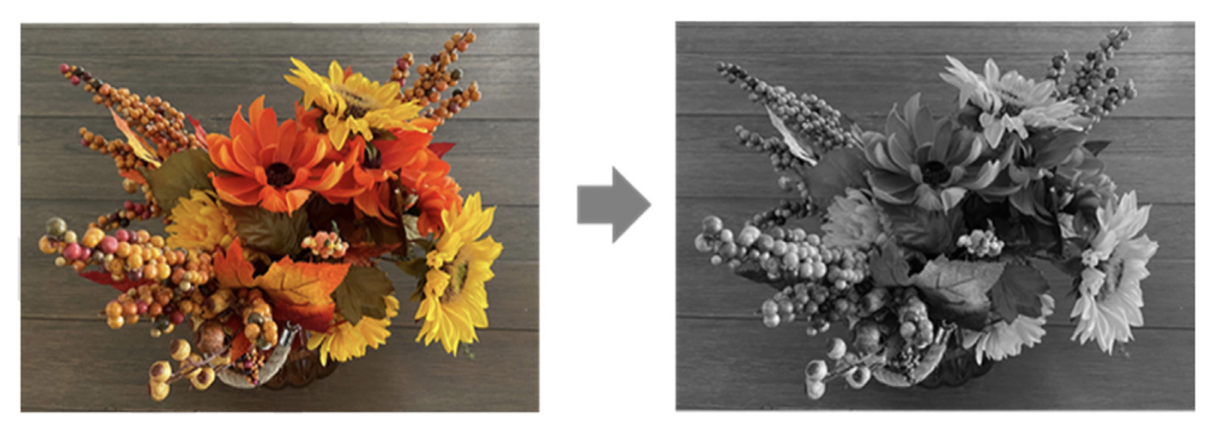
\includegraphics[width=0.9\textwidth]{figs/F2.1.png}
	\caption{\textit{将彩色图像转换为灰度图像。}}
\end{figure}

让我们通过一个彩色到灰度转换的例子来说明数据并行的概念。 图 2.1 显示了由许多像素组成的彩色图像(左侧),
每个像素包含从 0(黑色)到 1(全强度)变化的红色、绿色和蓝色分数值(r、g、b)。

为了将彩色图像(图 2.1 左侧)转换为灰度图像(右侧),我们通过应用以下加权和公式计算每个像素的亮度值 L:
\begin{equation*}
	L = r*0.21 + g*0.72 + b * 0.07
\end{equation*}

\begin{remark}[RGB 彩色图像表示]
在 RGB 表示中,图像中的每个像素都存储为 (r, g, b) 值的元组。 
图像行的格式为 (r g b) (r g b) ... (r g b),如下面的概念图所示。 
每个元组指定红色 (R)、绿色 (G) 和蓝色 (B) 的混合。 也就是说,
对于每个像素,r、g、b 值代表渲染该像素时红、绿、蓝光源的强度(0 为暗,1 为全强度)。
\begin{figure}[H]
	\centering
	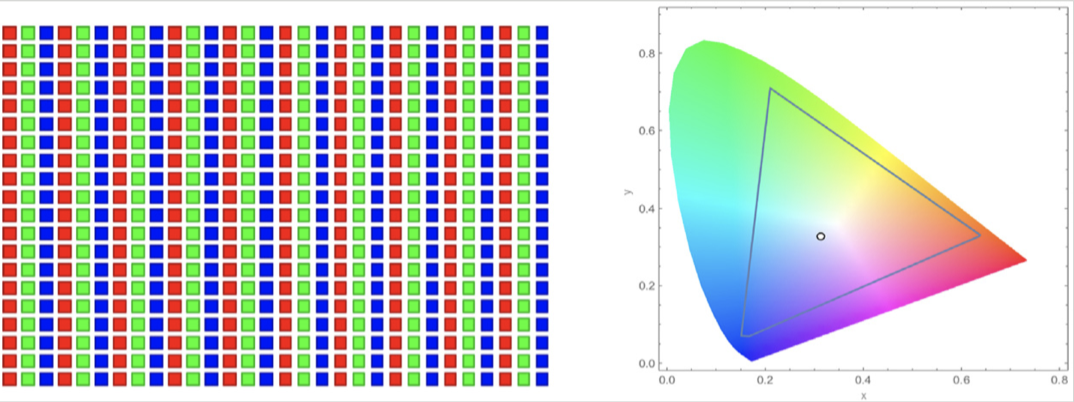
\includegraphics[width=0.9\textwidth]{figs/F2-a1.png}
\end{figure}

这三种颜色的实际允许混合因行业指定的颜色空间而异。 
这里,AdbobeRGB$^{TM}$ 颜色空间中三种颜色的有效组合显示为三角形的内部。 
每个混合的垂直坐标(y 值)和水平坐标(x 值)显示应为 G 和 R 的像素强度分数。像素强度的剩余分数 (1-y-x) 应分配给 B。 
渲染图像时,每个像素的 r、g、b 值用于计算像素的总强度(亮度)以及混合系数(x、y、1-y-x)。
\end{remark}

\begin{figure}[H]
	\centering
	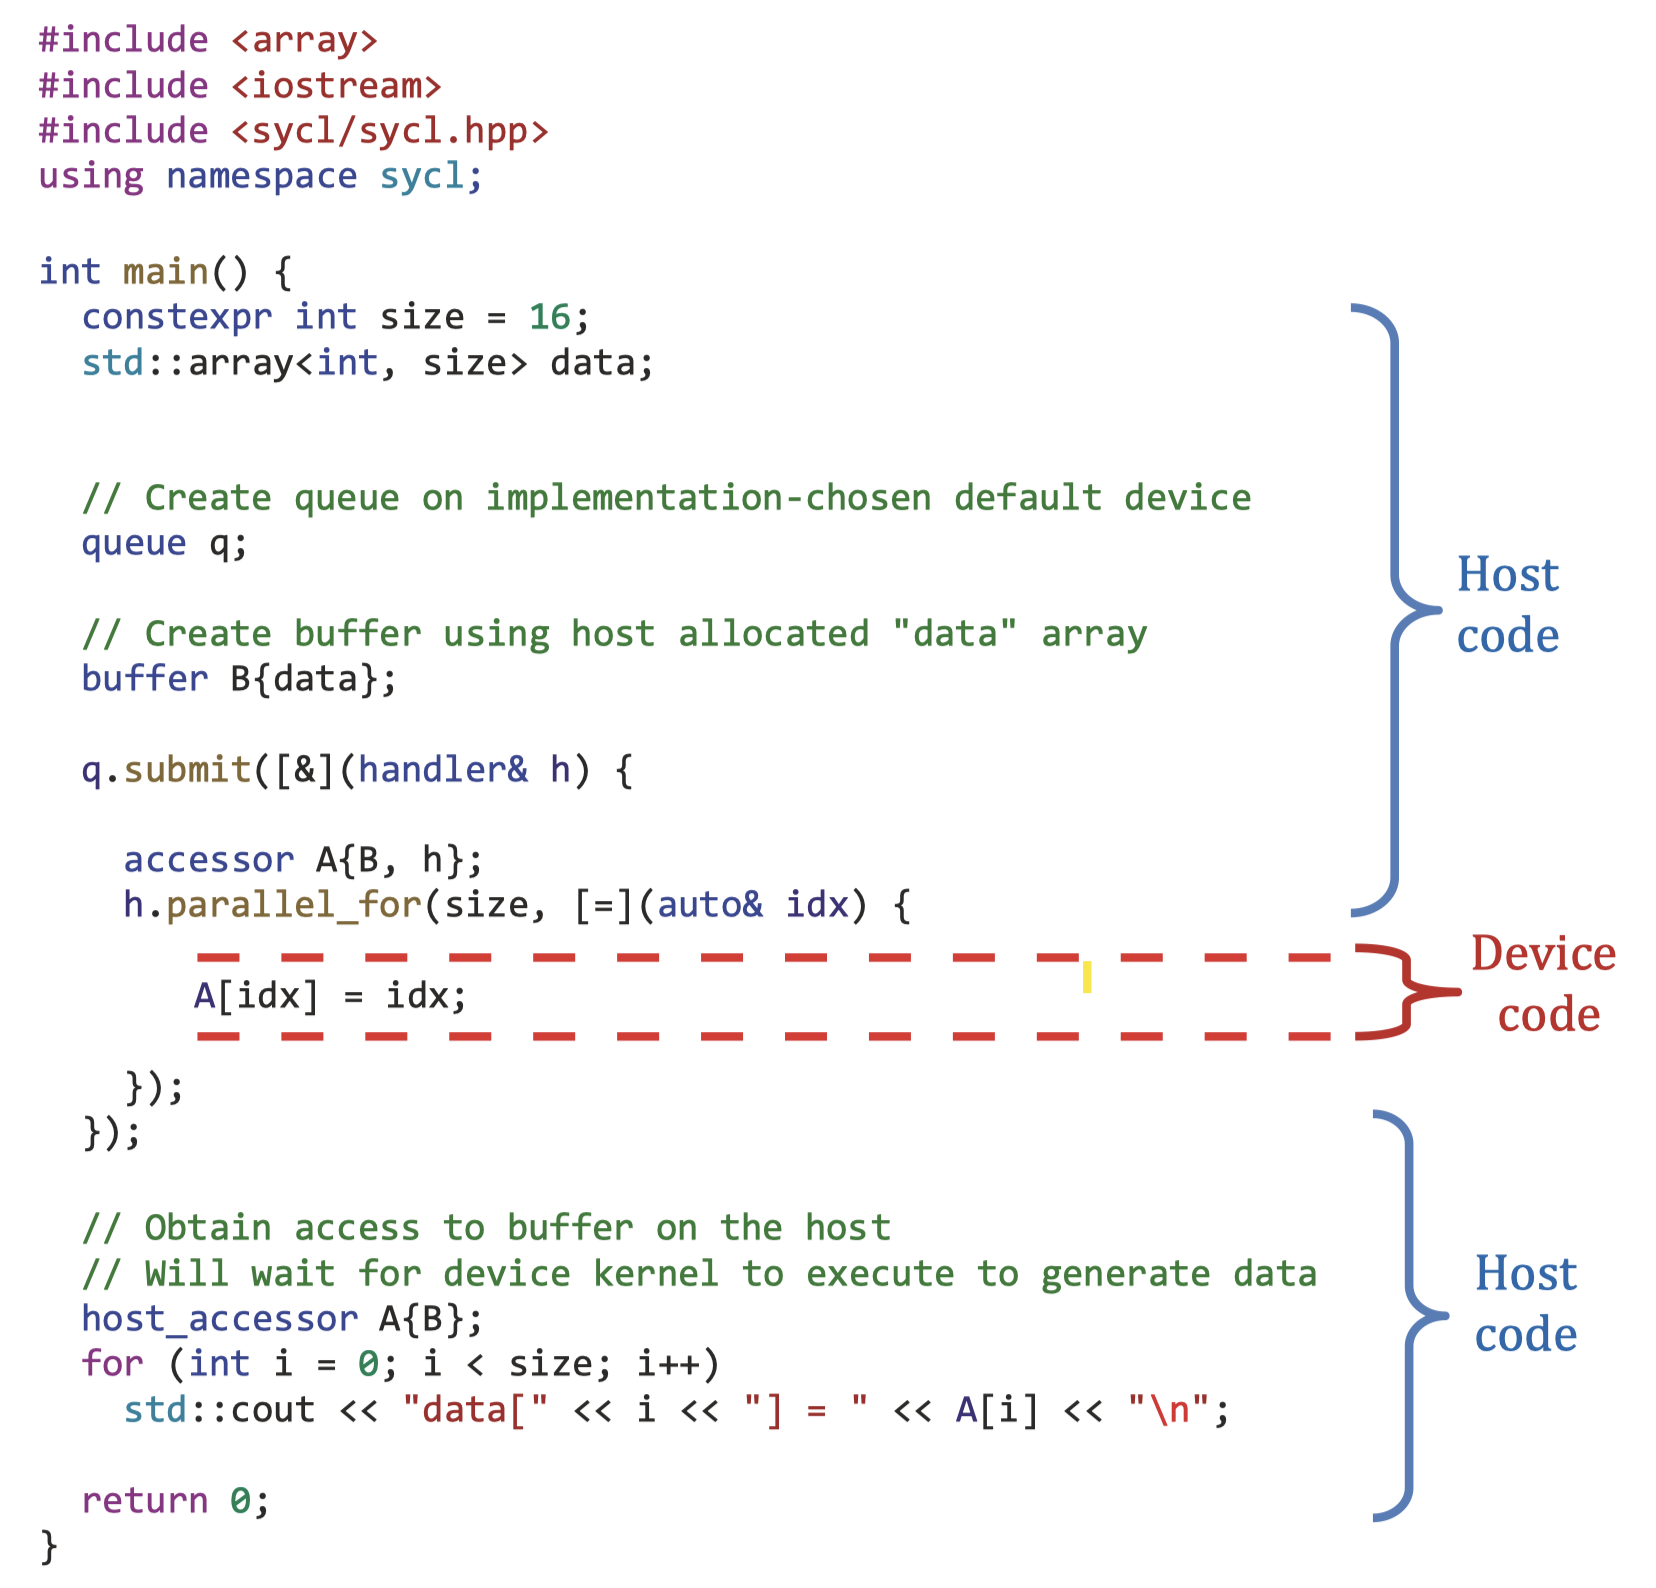
\includegraphics[width=0.9\textwidth]{figs/F2.2.png}
	\caption{\textit{图像到灰度转换中的数据并行性。 像素可以彼此独立地计算。}}
\end{figure}

如果我们将输入视为由 RGB 值数组 I 组织的图像,并将输出视为相应的亮度值数组 O,则我们得到如图 2.2 所示的简单计算结构。 
例如,根据上式计算I[0]中RGB值的加权和,生成O[0]; O[1]是通过计算I[1]中RGB值的加权和生成的; 
O[2]是通过计算I[2]中RGB值的加权和生成的; 等等。 这些每像素计算都不相互依赖。 所有这些都可以独立执行。 
显然,彩色到灰度的转换表现出丰富的数据并行性。 当然,完整应用程序中的数据并行性可能更加复杂,
本书的大部分内容都致力于教授发现和利用数据并行性所必需的并行思维。

\begin{remark}[任务并行与数据并行]
数据并行并不是并行编程中使用的唯一并行类型。 任务并行性也广泛应用于并行编程中。 
任务并行性通常通过应用程序的任务分解来暴露。 例如,一个简单的应用程序可能需要进行向量加法和矩阵向量乘法。 
其中每一个都是一项任务。 如果两个任务可以独立完成,则存在任务并行性。 I/O 和数据传输也是常见的任务源。

在大型应用程序中,通常存在大量独立任务,因此任务并行性也较大。 例如,在分子动力学模拟器中,
自然任务列表包括振动力、旋转力、非键合力的邻居识别、非键合力、速度和位置以及基于速度和位置的其他物理属性。

一般来说,数据并行性是并行程序可扩展性的主要来源。 对于大型数据集,人们通常可以找到丰富的数据并行性,
以便能够利用大规模并行处理器,并允许应用程序性能随着每一代具有更多执行资源的硬件而增长。 
尽管如此,任务并行性也可以在实现性能目标方面发挥重要作用。 稍后在介绍流(stream)时我们将介绍任务并行性。
\end{remark}

\subsection{CUDA C程序结构}
我们现在准备学习如何编写 CUDA C 程序来利用数据并行性来加快执行速度。 
CUDA C\footnote{CUDA C 采用 C++ 特性的趋势一直在稳步推进。 我们将在编程示例中使用其中一些 C++ 特性。} 
以最少的新语法和库函数扩展了流行的 ANSI C 编程语言,
使程序员能够针对包含 CPU 内核和大规模并行 GPU 的异构计算系统。 顾名思义,CUDA C 构建在 NVIDIA 的 CUDA 平台上。 
CUDA是目前最成熟的大规模并行计算框架。 它广泛应用于高性能计算行业,
在最常见的操作系统上提供编译器、调试器和分析器等基本工具。

CUDA C 程序的结构反映了计算机中主机(CPU)和一个或多个设备(GPU)的共存。 
每个 CUDA C 源文件可以混合有主机代码和设备代码。 默认情况下,任何传统 C 程序都是仅包含主机代码的 CUDA 程序。 
人们可以将设备代码添加到任何源文件中。 设备代码清楚地标有特殊的 CUDA C 关键字。 
设备代码包括函数或内核,其代码以数据并行方式执行。

\begin{figure}[H]
	\centering
	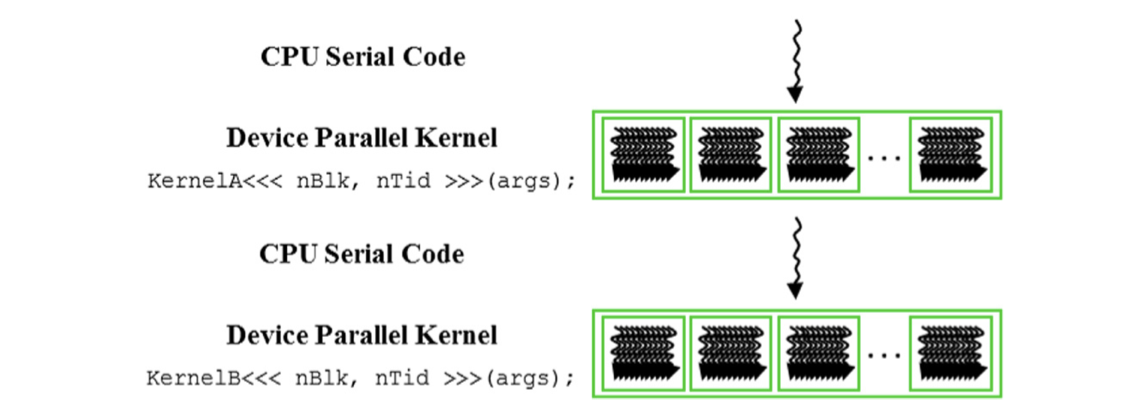
\includegraphics[width=0.9\textwidth]{figs/F2.3.png}
	\caption{\textit{CUDA 程序的执行。}}
\end{figure}

CUDA 程序的执行如图 2.3 所示。 执行从主机代码(CPU 串行代码)开始。 当调用内核函数时,
设备上会启动大量线程来执行内核。 由内核调用启动的所有线程统称为网格。 这些线程是 CUDA 平台中并行执行的主要工具。 
图 2.3 显示了两个线程网格的执行情况。 我们将很快讨论这些网格是如何组织的。 
当网格的所有线程都完成其执行时,网格终止,并且执行在主机上继续,直到启动另一个网格。 
请注意,图 2.3 显示了一个简化模型,其中 CPU 执行和 GPU 执行不重叠。 
许多异构计算应用程序管理重叠的 CPU 和 GPU 执行,以充分利用 CPU 和 GPU。

启动网格通常会生成许多线程来利用数据并行性。 在彩色到灰度转换的示例中,每个线程可用于计算输出数组 O 的一个像素。
在这种情况下,网格启动应生成的线程数等于 图片。 对于大图像,会产生大量线程。 
由于高效的硬件支持,CUDA 程序员可以假设这些线程只需很少的时钟周期即可生成和调度。 
这一假设与传统的 CPU 线程形成对比,传统的 CPU 线程通常需要数千个时钟周期来生成和调度。 
在下一章中,我们将展示如何实现颜色到灰度转换和图像模糊内核。 
在本章的其余部分中,为了简单起见,我们将使用向量加法作为运行示例。

\begin{remark}[线程]
线程是现代计算机中处理器如何执行顺序程序的简化视图。 线程由程序代码、正在执行的代码中的点及其变量和数据结构的值组成。 
就用户而言,线程的执行是顺序的。 人们可以使用源代码级调试器来监视线程的进度,
方法是一次执行一个语句,查看下一个将要执行的语句,并在执行过程中检查变量和数据结构的值。

线程在编程中的应用已经很多年了。 如果程序员想要在应用程序中开始并行执行,他/她可以使用线程库或特殊语言创建和管理多个线程。 
在 CUDA 中,每个线程的执行也是顺序的。 CUDA 程序通过调用内核函数来启动并行执行,
这会导致底层运行时机制启动并行处理数据不同部分的线程网格。
\end{remark}

\subsection{向量加法核函数}
\begin{figure}[H]
	\centering
	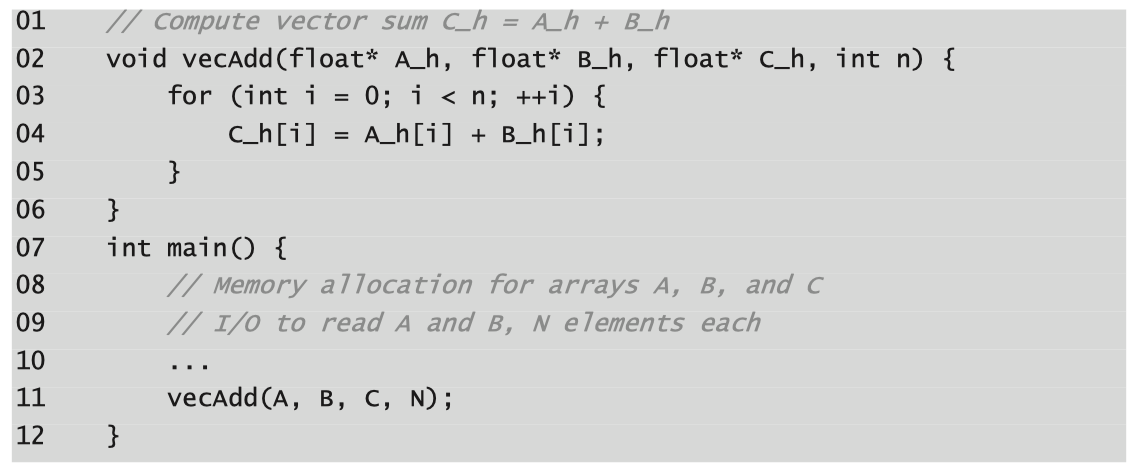
\includegraphics[width=0.9\textwidth]{figs/F2.4.png}
	\caption{\textit{一个简单的传统向量加法 C 代码示例。}}
\end{figure}

我们使用向量加法来演示 CUDA C 程序结构。 向量加法可以说是最简单的数据并行计算——相当于顺序编程中的“Hello World”。 
在我们展示向量加法的内核代码之前,首先回顾一下传统向量加法(主机代码)函数的工作原理会很有帮助。 
图 2.4 显示了一个简单的传统 C 程序,由主函数和向量加法函数组成。 在我们所有的示例中,每当需要区分主机和设备数据时,
我们都会在主机使用的变量名称后添加“\_h”,在设备使用的变量名称后添加“\_d”以 提醒我们自己这些变量的预期用途。 
由于图 2.4 中只有主机代码,因此我们只能看到后缀为“\_h”的变量。

\begin{remark}[C语言中的指针]
	图 2.4 中的函数参数 A、B 和 C 是指针。 在C语言中,可以使用指针来访问变量和数据结构。 浮点变量 V 可以这样声明:
	
float $V$;

指针变量 $P$ 可以这样声明:

float ${ }^{*} P$

通过使用语句 $P=\& V$ 将 $V$ 的地址分配给 $P$,我们使 $P$“指向”$V$。 ${ }^{*} P$ 成为 $V$ 的同义词。 
例如,$U={ }^{*} P$ 将$V$ 的值赋给$U$。 再例如, ${ }^{*} P=3$ 将 $V$ 的值更改为 3 。

$C$ 程序中的数组可以通过指向其 $O^{\text {th }}$ 元素的指针来访问。 
例如,语句 $P=\&(A[0])$ 使 $P$ 指向数组 A 的 $O^{\text {th }}$ 元素。 
P[i] 成为 A[i] 的同义词。 事实上,数组名称 $A$ 本身就是一个指向其 $O^{\text {th }}$ 元素的指针。

在图 2.4 中,将数组名 $A$ 作为函数调用的第一个参数传递给 vecAdd,
使得函数的第一个参数 $A \_h$ 指向 $A$ 的 $0^{\text {th }}$ 元素。 
因此,函数体中的 $A \_h[i]$ 可用于访问主函数中数组 $\mathrm{A}$ 的 $A[i]$。

请参阅 Patt \& Patel(Patt \& Patel,2020),了解 $C$ 中指针的详细用法的简单易懂的解释。
\end{remark}

假设要相加的向量存储在主程序中分配并初始化的数组A和B中。 输出向量位于数组C中,该数组也在主程序中分配。 
为了简洁起见,我们没有显示 A、B 和 C 在主函数中如何分配或初始化的细节。 
指向这些数组的指针连同包含向量长度的变量 N 一起传递给 vecAdd 函数。 
请注意,vecAdd 函数的参数带有“\_h”后缀,以强调它们是由主机使用的。 
当我们在接下来的几个步骤中引入设备代码时,这种命名约定将会很有帮助。

图 2.4 中的 vecAdd 函数使用 for 循环来迭代向量元素。 在第 i 次迭代中,
输出元素 C\_h[i] 接收 A\_h[i] 和 B\_h[i] 的和。 向量长度参数 n 用于控制循环,使迭代次数与向量的长度相匹配。 
该函数分别通过指针A\_h、B\_h和C\_h读取A和B的元素并写入C的元素。 
当vecAdd函数返回时,main函数中的后续语句就可以访问C的新内容。

\begin{figure}[H]
	\centering
	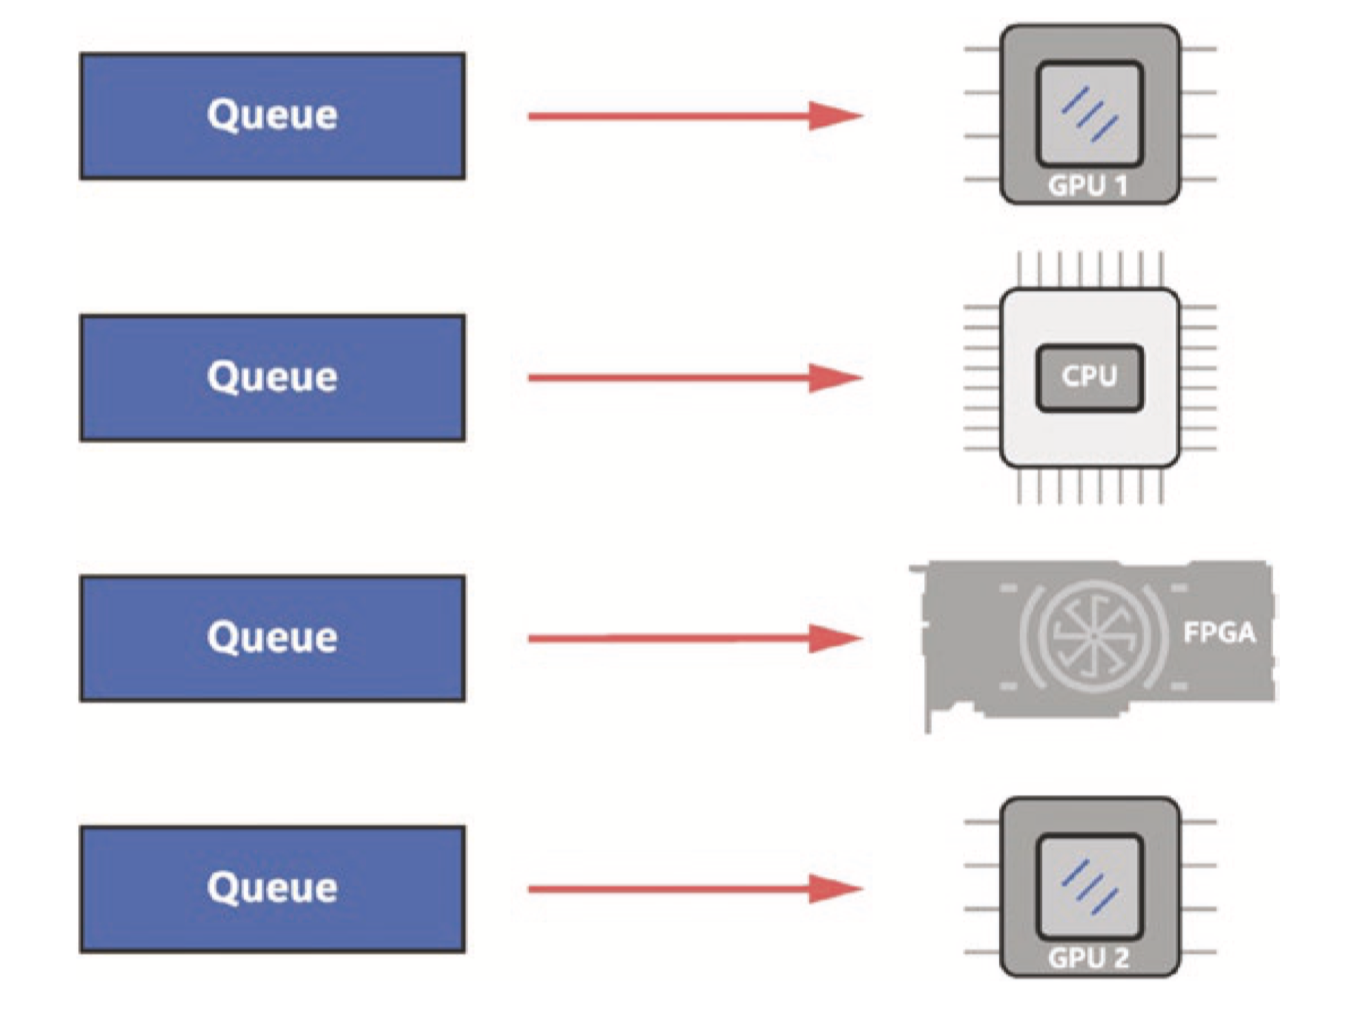
\includegraphics[width=0.9\textwidth]{figs/F2.5.png}
	\caption{\textit{将工作移至设备的修订版 vecAdd 函数的概述。}}
\end{figure}

并行执行向量加法的一种直接方法是修改 vecAdd 函数并将其计算移至设备。 这种修改后的 vecAdd 函数的结构如图 2.5 所示。 
该函数的第 1 部分在设备 (GPU) 内存中分配空间来保存 A、B 和 C 向量的副本,并将 A 和 B 向量从主机内存复制到设备内存。 
第 2 部分调用实际的向量加法内核来启动设备上的线程网格。 
第 3 部分将和向量 C 从设备内存复制到主机内存,并从设备内存中释放三个数组。

请注意,修改后的 vecAdd 函数本质上是一个外包代理,它将输入数据发送到设备,激活设备上的计算,并从设备收集结果。 
代理这样做的方式是主程序甚至不需要知道矢量加法现在实际上是在设备上完成的。 在实践中,这种“透明”的外包模式可能非常低效,
因为所有数据都来回复制。 人们通常会在设备上保留大型且重要的数据结构,并简单地从主机代码中调用它们上的设备功能。 
不过,现在我们将使用简化的透明模型来介绍基本的 CUDA C 程序结构。 
修改后的函数的细节以及内核函数的编写方式将是本章剩余部分的主题。

\subsection{设备全局内存和数据传输}
在当前的 CUDA 系统中,设备通常是硬件卡,带有自己的动态随机存取存储器,称为设备全局存储器,或简称为全局存储器。 
例如,NVIDIA Volta V100 配备 16GB 或 32GB 全局内存。 将其称为“全局”内存,
将其与程序员也可以访问的其他类型的设备内存区分开来。 
有关 CUDA 内存模型和不同类型设备内存的详细信息将在第 5 章“内存架构和数据局部性”中讨论。

对于向量加法内核,在调用内核之前,程序员需要在设备全局内存中分配空间,并将数据从主机内存传输到设备全局内存中分配的空间。 
这对应于图 2.5 的第 1 部分。 类似地,在设备执行之后,程序员需要将结果数据从设备全局存储器传输回主机存储器,
并释放设备全局存储器中不再需要的已分配空间。 这对应于图 2.5 的第 3 部分。 
CUDA运行时系统(通常在主机上运行)提供应用程序编程接口(API)函数来代表程序员执行这些活动。 
从现在开始,我们将简单地说数据从主机传输到设备,作为数据从主机内存复制到设备全局内存的简写。 对于相反的方向也是如此。

图2.5中,vecAdd函数的第1部分和第3部分需要使用CUDA API函数为A、B和C分配设备全局内存; 
将 A 和 B 从主机传输到设备; 向量相加后将 C 从设备传输到主机; 并释放A、B、C的设备全局内存。
我们首先解释内存分配和释放函数。

\begin{figure}[H]
	\centering
	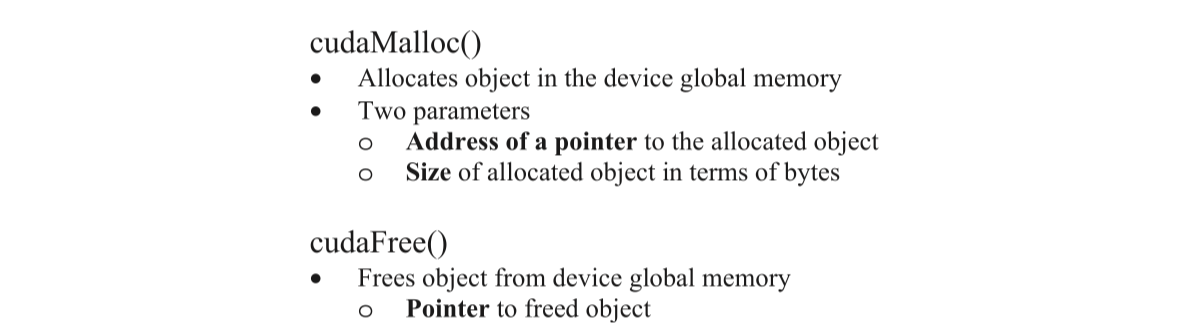
\includegraphics[width=0.9\textwidth]{figs/F2.6.png}
	\caption{\textit{用于管理设备全局内存的 CUDA API 函数。}}
\end{figure}

图 2.6 显示了两个用于分配和释放设备全局内存的 API 函数。 
可以从主机代码调用 cudaMalloc 函数来为对象分配一块设备全局内存。 
读者应该注意到 cudaMalloc 和标准 C 运行时库 malloc 函数之间惊人的相似性。 
这是故意的; CUDA C 是具有最少扩展的 C。 CUDA C使用标准C运行时库malloc函数来管理主机内存
\footnote{CUDA C 还具有更高级的库函数,用于在主机内存中分配空间。 我们将在第 20 章“异构计算集群编程”中讨论它们。} ,
并将cudaMalloc作为C运行时库的扩展添加。 通过使接口尽可能接近原始 C 运行时库,
CUDA C 最大限度地减少了 C 程序员重新学习这些扩展的使用所花费的时间。

cudaMalloc 函数的第一个参数是指针变量的地址,该变量将被设置为指向分配的对象。
指针变量的地址应转换为 (void ** ),因为该函数需要一个通用指针; 内存分配函数是一个通用函数,不限于任何特定类型的对象
\footnote{cudaMalloc 返回通用对象这一事实使得动态分配的多维数组的使用更加复杂。 我们将在 3.2 节中解决这个问题。} 。
该参数允许 cudaMalloc 函数将分配的内存的地址写入提供的指针变量,无论其类型如何
\footnote{请注意,cudaMalloc 的格式与 C malloc 函数不同。 C malloc 函数返回指向已分配对象的指针。 
它只需要一个参数来指定分配对象的大小。 cudaMalloc 函数写入地址作为第一个参数给出的指针变量。 
因此,cudaMalloc 函数有两个参数。 
cudaMalloc 的双参数格式允许它使用返回值以与其他 CUDA API 函数相同的方式报告任何错误。}。
调用内核的主机代码将此指针值传递给需要访问已分配内存对象的内核。 
cudaMalloc 函数的第二个参数给出要分配的数据的大小(以字节数为单位)。 
第二个参数的用法与 C malloc 函数的大小参数一致。

我们现在用下面简单的代码示例来说明cudaMalloc和cudaFree的使用:

float *A\_d 

int size=n * sizeof(float);

cudaMalloc((void ** )\&A\_d, size);

... cudaFree(A\_d);

这是图 2.5 中示例的延续。 为了清楚起见,我们在指针变量后面加上“\_d”后缀,以指示它指向设备全局内存中的对象。 
传递给 cudaMalloc 的第一个参数是转换为 void 指针的指针 A\_d(即 \&A\_d)的地址。 
当cudaMalloc返回时,A\_d将指向为A向量分配的设备全局内存区域。 传递给 cudaMalloc 的第二个参数是要分配的区域的大小。 
由于 size 是以字节数为单位的,因此程序员在确定 size 的值时需要将数组中的元素数转换为字节数。 
例如,在为包含 n 个单精度浮点元素的数组分配空间时,size 的值将是单精度浮点数大小的 n 倍,在当今的计算机中为 4 个字节。 
因此,size 的值将为 n × 4。计算后,以指针 A\_d 作为参数调用 cudaFree,以从设备全局内存中释放 A 向量的存储空间。 
注意cudaFree不需要改变A\_d的值; 它只需要使用A\_d的值将分配的内存返回到可用池。 
因此,只有 A\_d 的值而不是地址作为参数传递。

A\_d、B\_d 和 C\_d 中的地址指向设备全局内存中的位置。 这些地址不应在主机代码中取消引用。 
它们应该用于调用API函数和内核函数。 在主机代码中取消引用设备全局内存指针可能会导致异常或其他类型的运行时错误。

读者应该使用类似的 B\_d 和 C\_d 指针变量声明及其相应的 cudaMalloc 调用来完成图 2.5 中 vecAdd 示例的第 1 部分。 
此外,图 2.5 中的第 3 部分可以通过调用 B\_d 和 C\_d 的 cudaFree 来完成。

\begin{figure}[H]
	\centering
	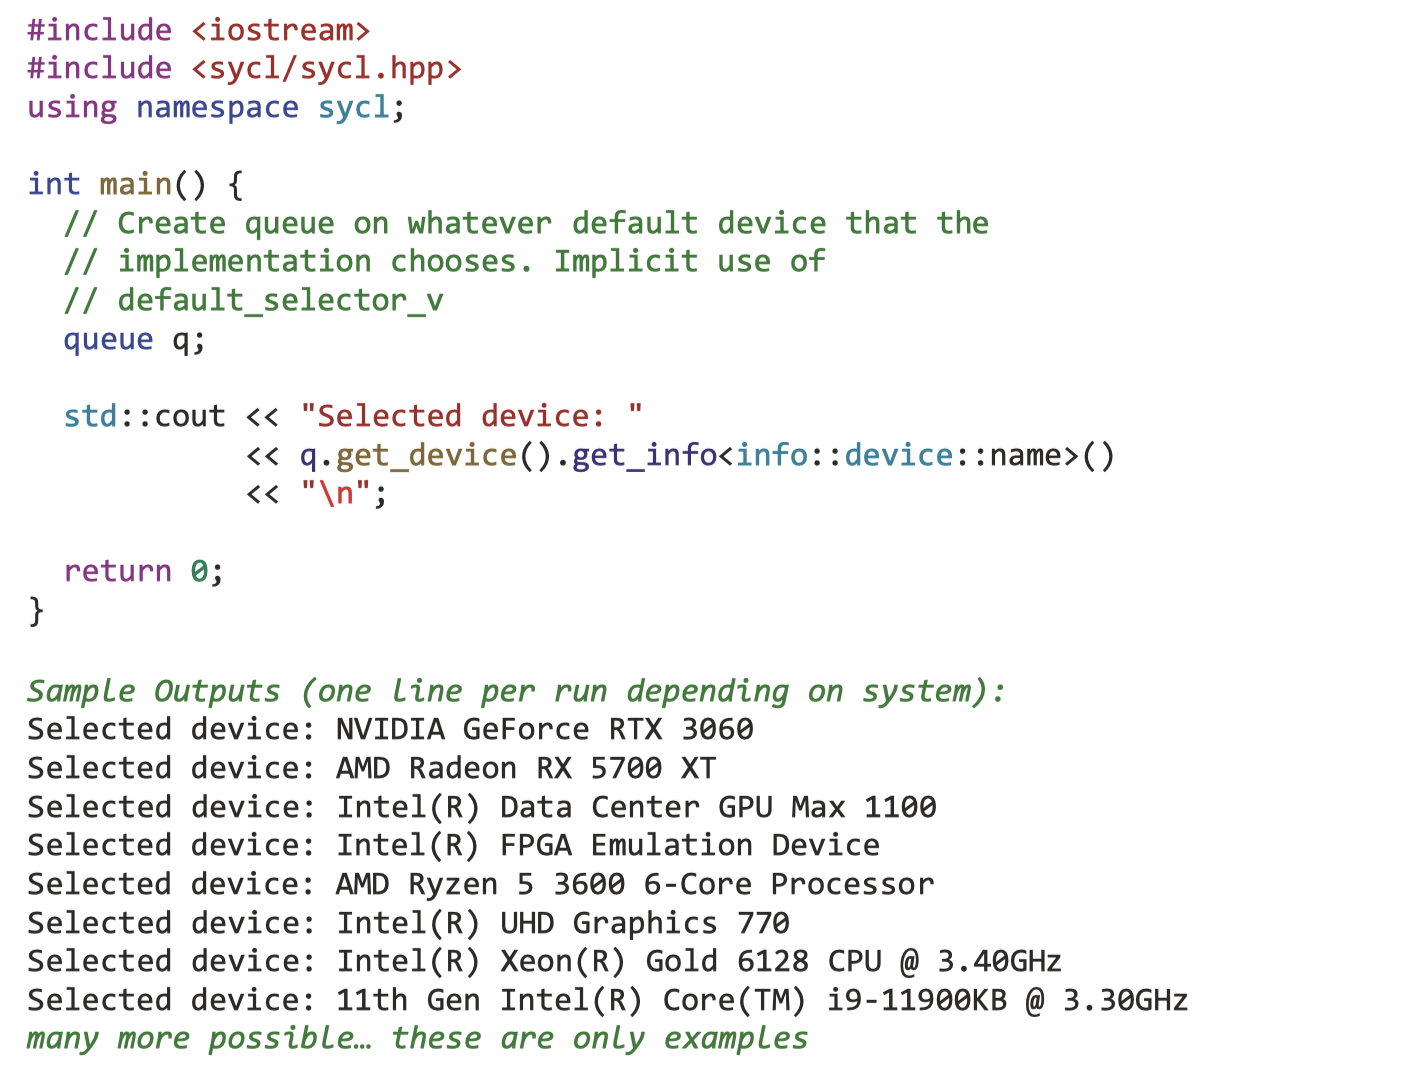
\includegraphics[width=0.9\textwidth]{figs/F2.7.png}
	\caption{\textit{CUDA API 函数用于主机和设备之间的数据传输。}}
\end{figure}

一旦主机代码在设备全局存储器中为数据对象分配了空间,它就可以请求将数据从主机传输到设备。 
这是通过调用 CUDA API 函数之一来完成的。 图 2.7 显示了这样一个 API 函数 cudaMemcpy。 
cudaMemcpy 函数有四个参数。 第一个参数是指向要复制的数据对象的目标位置的指针。 第二个参数指向源位置。 
第三个参数指定要复制的字节数。 第四个参数表示复制涉及的内存类型:从主机到主机、从主机到设备、从设备到主机、从设备到设备。 
例如,存储器复制功能可用于将数据从设备全局存储器中的一个位置复制到设备全局存储器中的另一位置。

vecAdd 函数调用 cudaMemcpy 函数,在相加之前将 A\_h 和 B\_h 向量从主机内存复制到设备内存中的 A\_d 和 B\_d,
并在相加完成后将 C\_d 向量从设备内存复制到主机内存中的 C\_h 完毕。 
假设 A\_h、B\_h、A\_d、B\_d 和 size 的值已经按照我们之前讨论的那样设置,则三个 cudaMemcpy 调用如下所示。 
两个符号常量 cudaMemcpyHostToDevice 和 cudaMemcpyDeviceToHost 是 CUDA 编程环境可识别的预定义常量。 
请注意,通过正确排序源指针和目标指针并使用适合传输类型的常量,可以使用同一函数在两个方向上传输数据。

cudaMemcpy(A\_d, A\_h, size, cudaMemcpyHostToDevice); 

cudaMemcpy(B\_d, B\_h, size, cudaMemcpyHostToDevice); 

...

cudaMemcpy(C\_h, C\_d, size, cudaMemcpyDeviceToHost);

总而言之,图2.4中的主程序调用vecAdd,它也在主机上执行。 vecAdd 函数如图 2.5 所示,在设备全局内存中分配空间,
请求数据传输,并调用执行实际向量加法的内核。 我们将这种类型的主机代码称为调用内核的存根。 
我们在图 2.8 中展示了 vecAdd 函数的更完整版本。

\begin{figure}[H]
	\centering
	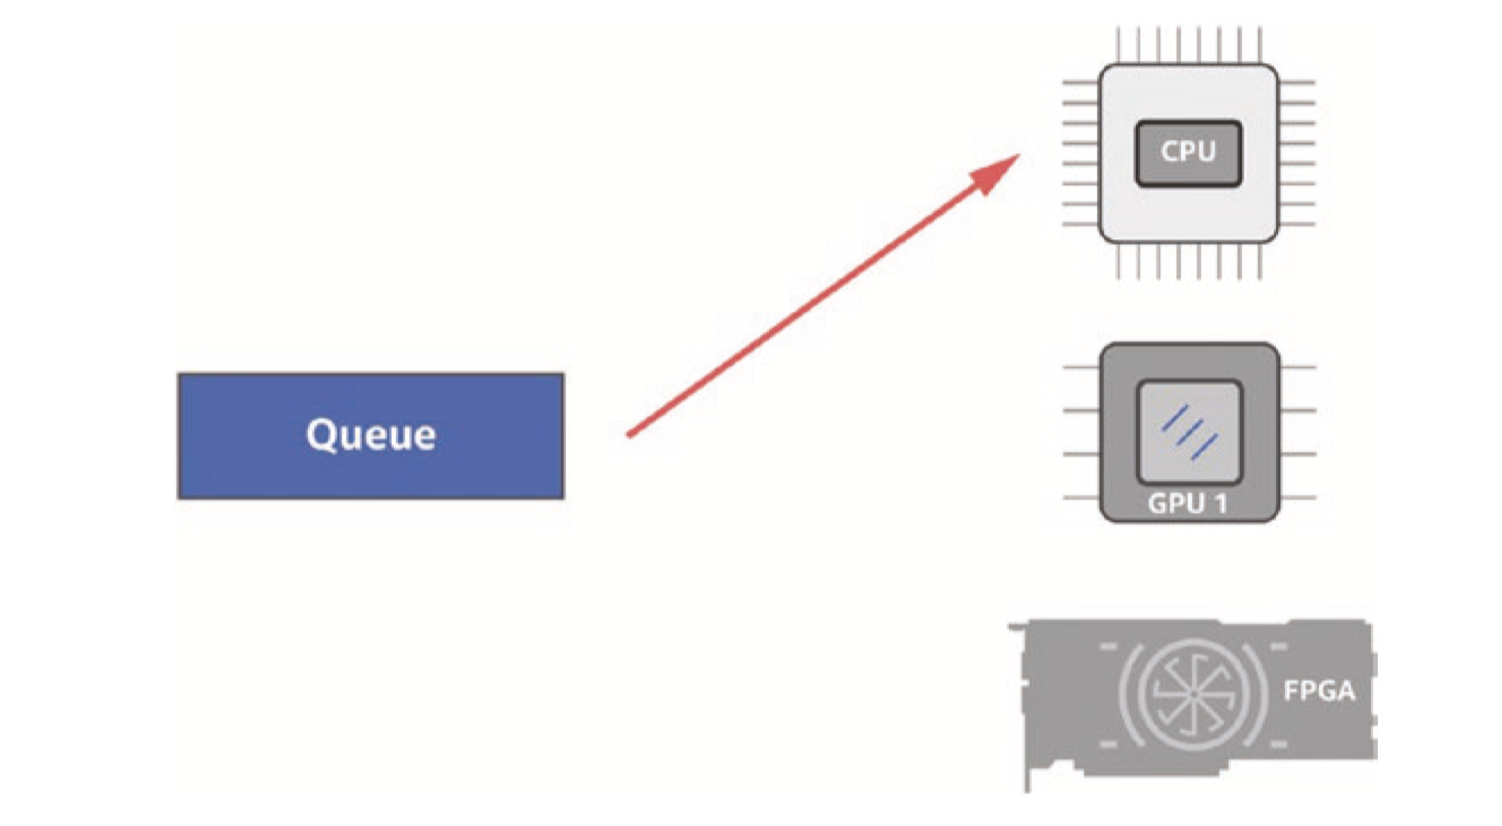
\includegraphics[width=0.9\textwidth]{figs/F2.8.png}
	\caption{\textit{vecAdd() 的更完整版本。}}
\end{figure}

与图2.5相比,图2.8中的vecAdd函数对于第1部分和第3部分来说是完整的。第1部分为A\_d、B\_d和C\_d分配设备全局内存,
并将A\_h传输到A\_d,将B\_h传输到B\_d。 这是通过调用 cudaMalloc 和 cudaMemcpy 来完成的功能。 
鼓励读者使用适当的参数值编写自己的函数调用,并将他们的代码与图 2.8 所示的代码进行比较。 
第 2 部分调用内核,并将在下面的小节中描述。 第 3 部分将向量和数据从设备复制到主机,以便这些值在主函数中可用。 
这是通过调用 cudaMemcpy 函数来完成的。 然后,它从设备全局内存中释放 A\_d、B\_d 和 C\_d 的内存,
这是通过调用 cudaFree 函数来完成的(图 2.9)。

\begin{remark}[CUDA 中的错误检查和处理]
	一般来说,检查和处理错误对于程序来说很重要。 CUDA API 函数返回标志,指示它们在处理请求时是否发生错误。 
	大多数错误是由于调用中使用的参数值不正确造成的。
	
为简洁起见,我们不会在示例中显示错误检查代码。 例如,图 2.9 显示了对 cudaMalloc 的调用:

cudaMalloc((void $\left.{ }^{* *}\right) \& A \_d$, size $)$;

在实践中,我们应该用测试错误条件的代码包围调用并打印出错误消息,以便用户可以知道发生了错误。 此类检查代码的简单版本如下:

cudaError\_t err = cudaMalloc((void**) \&A\_d, size);

if (error != cudaSuccess) \{

	printf(“\%s in \%s at line \%d \textbackslash n”, 
	        cudaGetErrorString(err), \_\_FILE\_\_, \_\_LINE\_\_);

	exit(EXIT\_FAILURE); 

\}

这样,如果系统的设备内存不足,用户将收到有关情况的通知。 这可以节省许多小时的调试时间。

可以定义一个 $C$ 宏来使源代码中的检查代码更加简洁。
\end{remark}

\subsection{核函数与线程}
我们现在准备更多地讨论 CUDA C 内核函数以及调用这些内核函数的效果。 在 CUDA C 中,
内核函数指定在并行阶段由所有线程执行的代码。 由于所有这些线程都执行相同的代码,
因此 CUDA C 编程是著名的单程序多数据 (SPMD)(Atallah,1998)并行编程风格的一个实例,
这是并行计算系统的一种流行编程风格\footnote{请注意,SPMD 与 SIMD(单指令多数据)不同 [Flynn 1972]。 
在 SPMD 系统中,并行处理单元对数据的多个部分执行相同的程序。 然而,这些处理单元不需要同时执行相同的指令。 
在 SIMD 系统中,所有处理单元在任何时刻都执行相同的指令。} 。

当程序的主机代码调用内核时,CUDA 运行时系统会启动组织成两级层次结构的线程网格。 每个网格都组织为线程块数组,
为简洁起见,我们将其称为块。 网格中的所有块的大小相同; 在当前系统上,每个块最多可以包含 1024 个线程
\footnote{在 CUDA 3.0 及更高版本中,每个线程块最多可以有 1024 个线程。 
一些早期的 CUDA 版本仅允许块中最多 512 个线程。} 。 
图 2.9 显示了一个示例,其中每个块由 256 个线程组成。 
每个线程都由一个来自方框的卷曲箭头表示,该方框标有块中线程的索引号。

\begin{figure}[H]
	\centering
	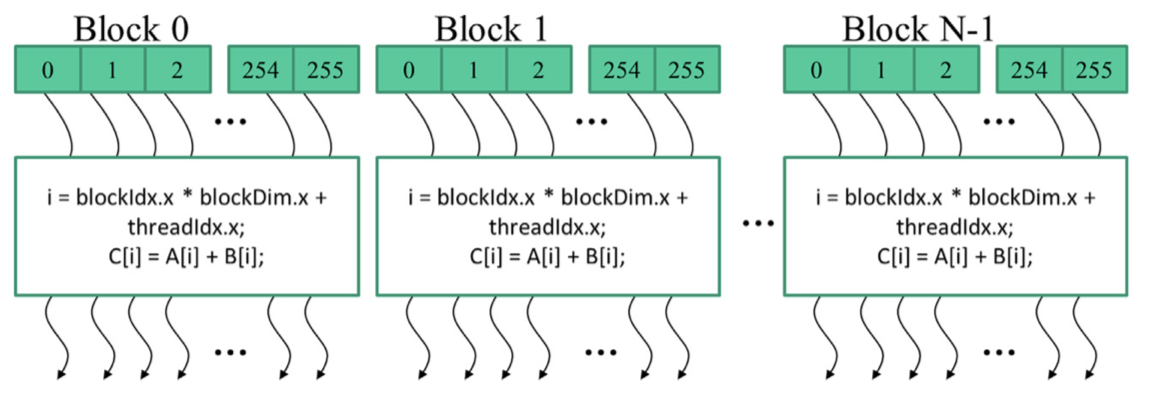
\includegraphics[width=0.9\textwidth]{figs/F2.9.png}
	\caption{\textit{网格中的所有线程都执行相同的内核代码。}}
\end{figure}

\begin{remark}[内置变量]
	许多编程语言都有内置变量。 这些变量具有特殊的含义和目的。 
	这些变量的值通常由运行时系统预先初始化,并且在程序中通常是只读的。 程序员应避免出于任何其他目的重新定义这些变量。
\end{remark}

每个线程块中的线程总数由调用内核时的主机代码指定。 可以在主机代码的不同部分使用不同数量的线程来调用相同的内核。 
对于给定的线程网格,块中的线程数可在名为 blockDim 的内置变量中获得。 
blockDim 变量是一个具有三个无符号整数字段(x、y 和 z)的结构,可帮助程序员将线程组织成一维、二维或三维数组。 
对于一维组织,仅使用 x 字段。 对于二维组织,使用 x 和 y 字段。 对于三维结构,使用所有三个 x、y 和 z 字段。 
组织线程的维度选择通常反映了数据的维度。 这是有道理的,因为创建线程是为了并行处理数据,
因此线程的组织很自然地反映了数据的组织。 在图2.9中,每个线程块被组织为一维线程数组,因为数据是一维向量。 
blockDim.x变量的值表示每个块中的线程总数,在图2.9中为256。 
一般来说,出于硬件效率的考虑,建议线程块每个维度的线程数量为32的倍数。 我们稍后会再讨论这个问题。

CUDA 内核可以访问另外两个内置变量(threadIdx 和 blockIdx),
这些变量允许线程彼此区分并确定每个线程要处理的数据区域。 threadIdx 变量为每个线程提供块内的唯一坐标。 
在图2.9中,由于我们使用一维线程组织,因此仅使用threadIdx.x。 
每个线程的 threadIdx.x 值显示在图 2.9 中每个线程的小阴影框中。 每个块中的第一个线程的 threadIdx.x 变量的值为 0,
第二个线程的值为 1,第三个线程的值为 2,依此类推。

\begin{remark}[层级组织]
与 CUDA 线程一样,许多现实世界的系统都是分层组织的。 美国的电话系统就是一个很好的例子。 
在顶层,电话系统由“区域”组成,每个区域对应一个地理区域。 同一区域内的所有电话线路都具有相同的 3 位数“区号”。 
电话区有时比城市还要大。 例如,伊利诺伊州中部的许多县市都在同一个电话区域内,并且共享相同的区号217。
在一个区域内,每条电话线都有一个七位数字的本地电话号码,这使得每个区域最多可以拥有约 一千万个数字。

可以将每条电话线视为一个 CUDA 线程,其中 blockIdx 的值为区号,threadIdx 的值为七位本地号码。 
这种分层组织允许系统拥有大量电话线路,同时保留呼叫同一区域的“局部性”。 
即拨打同一地区的电话线路时,只需拨打本地号码即可。 只要我们大部分的电话都是在本地拨打,很少需要拨打区号。 
如果我们偶尔需要拨打另一个地区的电话线,我们拨打 1 和区号,然后拨打本地号码。 
(这就是为什么任何区域中的本地编号都不应以 1 开头的原因。)CUDA 线程的分层组织还提供了一种局部性形式。 
我们很快就会研究这个地方。
\end{remark}

blockIdx 变量为块中的所有线程提供一个公共块坐标。 在图 2.9 中,第一个块中的所有线程的 blockIdx.x 变量的值为 0,
第二个线程块中的所有线程的值为 1,依此类推。 与电话系统进行类比,我们可以将 threadIdx.x 视为本地电话号码,
将 blockIdx.x 视为区号。 两者共同为全国的每条电话线提供了唯一的电话号码。 
类似地,每个线程可以组合其 threadIdx 和 blockIdx 值,在整个网格中为自己创建唯一的全局索引。

在图 2.9 中,唯一的全局索引 i 的计算公式为 i=blockIdx.x × blockDim.x + ThreadIdx.x。 
回想一下,在我们的示例中,blockDim 是 256。 块 0 中线程的 i 值范围是 0 到 255。 
块 1 中线程的 i 值范围是 256 到 511。 块 2 中线程的 i 值范围是 512 到 767。 
这三个块中的线程形成了从 0 到 767 的值的连续覆盖。由于每个线程使用 i 访问 A、B 和 C,
因此这些线程覆盖了原始循环的前 768 次迭代。 通过启动具有更多块的网格,可以处理更大的向量。 
通过启动具有 n 个或更多线程的网格,可以处理长度为 n 的向量。

\begin{figure}[H]
	\centering
	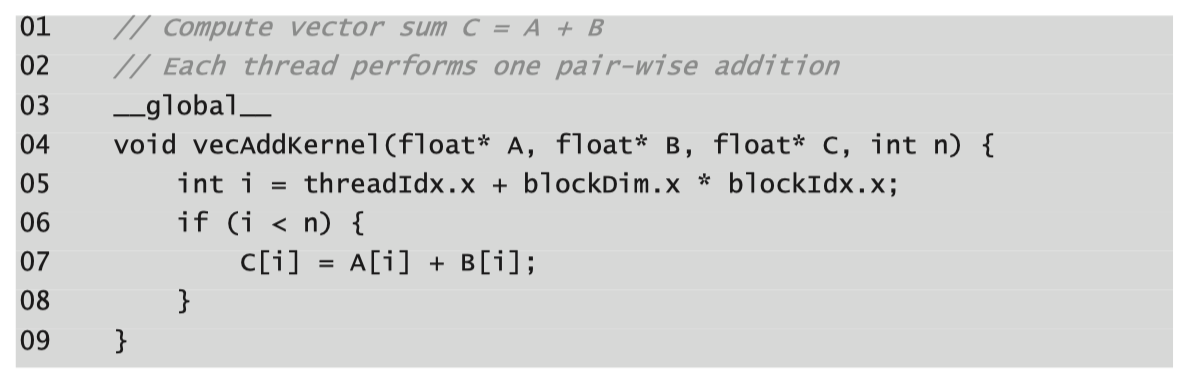
\includegraphics[width=0.9\textwidth]{figs/F2.10.png}
	\caption{\textit{向量加法核函数。}}
\end{figure}

图 2.10 显示了向量加法的核函数。 请注意,我们不在内核中使用“\_h”和“\_d”约定,因为不存在潜在的混淆。 
在我们的示例中,我们将无法访问主机内存。 内核的语法是 ANSI C,并带有一些值得注意的扩展。 
首先,在 vecAddKernel 函数的声明前面有一个 CUDA-C 特定关键字“\_\_global\_\_”。 
该关键字指示该函数是一个内核,并且可以调用它来在设备上生成线程网格。

\begin{figure}[H]
	\centering
	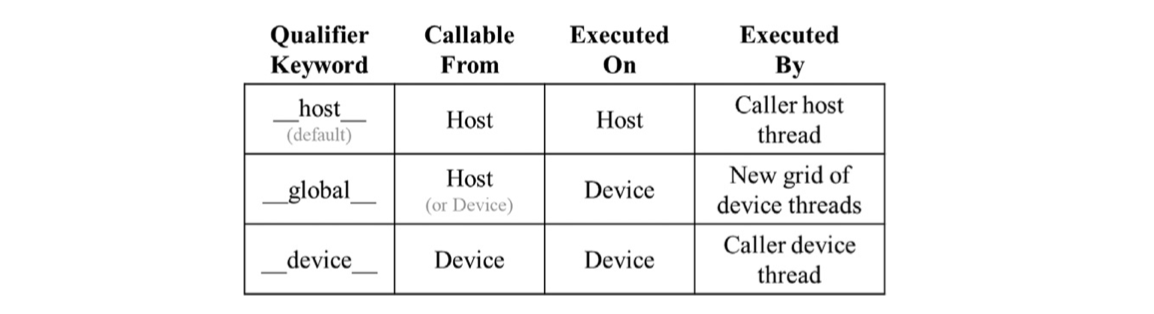
\includegraphics[width=0.9\textwidth]{figs/F2.11.png}
	\caption{\textit{用于函数声明的 CUDA C 关键字。}}
\end{figure}

一般来说,CUDA C 使用三个可在函数声明中使用的限定符关键字扩展了 C 语言。 
这些关键字的含义总结在图 2.11 中。 “\_\_global\_\_”关键字表示所声明的函数是 CUDA C 内核函数。 
请注意,“global”一词的两侧各有两个下划线字符。 这样的内核函数在设备上执行并且可以从主机调用。 
在支持动态并行的 CUDA 系统中,也可以从设备调用它,我们将在第 21 章“CUDA 动态并行”中看到。 
重要的特征是调用这样的内核函数会导致在设备上启动新的线程网格。

“\_\_device\_\_”关键字表示所声明的函数是 CUDA 设备函数。 设备函数在 CUDA 设备上执行,
并且只能从内核函数或其他设备函数调用。 设备函数由调用它的设备线程执行,不会导致启动任何新的设备线程
\footnote{稍后我们将解释不同代 CUDA 中使用间接函数调用和递归的规则。 
一般来说,应该避免在其设备函数和内核函数中使用递归和间接函数调用,以实现最大的可移植性。} 。

“\_\_host\_\_”关键字表示所声明的函数是 CUDA 主机函数。 主机函数只是在主机上执行的传统 C 函数,
并且只能从另一个主机函数调用。 默认情况下,如果 CUDA 程序中的所有函数在其声明中没有任何 CUDA 关键字,
则它们都是主机函数。 这是有道理的,因为许多 CUDA 应用程序都是从纯 CPU 执行环境移植的。 
程序员在移植过程中会添加内核函数和设备函数。 原始功能仍作为主机功能。 
将所有函数默认为主机函数可以使程序员免去更改所有原始函数声明的繁琐工作。

请注意,可以在函数声明中同时使用“\_\_host\_\_”和“\_\_device\_\_”。 
这种组合告诉编译系统为同一函数生成两个版本的目标代码。 一种是在主机上执行的,并且只能从主机函数中调用。 
另一个在设备上执行,只能从设备或内核函数中调用。 当可以重新编译相同的函数源代码以生成设备版本时,这支持常见的用例。 
许多用户库函数可能属于这一类。

C 的第二个值得注意的扩展,如图 2.10 所示,是内置变量“threadIdx”, “blockIdx”和“blockDim”。 
回想一下,所有线程都执行相同的内核代码,并且需要有一种方法让它们彼此区分并将每个线程引导至数据的特定部分。 
这些内置变量是线程访问为线程提供识别坐标的硬件寄存器的方法。 
不同的线程将在其 threadIdx.x, blockIdx.x 和 blockDim.x 变量中看到不同的值。 
为了便于阅读,我们有时会在讨论中将线程称为线程 blockIdx.x, threadIdx.x。

图 2.10 中有一个自动(局部)变量 i。 在 CUDA 内核函数中,自动变量是每个线程私有的。 
也就是说,将为每个线程生成一个 i 版本。 如果网格以 10,000 个线程启动,则 i 将会有 10,000 个版本,每个线程一个。 
线程为其 i 变量分配的值对其他线程不可见。 我们将在第 5 章“内存架构和数据局部性”中更详细地讨论这些自动变量。

快速比较图 2.4 和图 2.10 揭示了对 CUDA 内核的重要见解。 图 2.10 中的核函数没有与图 2.4 中的循环相对应的循环。 
读者应该问循环去了哪里。 答案是循环现在被线程网格所取代。 整个网格相当于循环。 网格中的每个线程对应于原始循环的一次迭代。 
这有时称为循环并行,其中原始顺序代码的迭代由线程并行执行。

注意图 2.10 中的 addVecKernel 中有一个 if(i < n) 语句。 这是因为并非所有向量长度都可以表示为块大小的倍数。 
例如,假设向量长度为 100。最小有效线程块维度为 32。假设我们选择 32 作为块大小。 
需要启动 4 个线程块来处理所有 100 个向量元素。 然而,四个线程块将有 128 个线程。 
我们需要禁止线程块 3 中的最后 28 个线程执行原始程序未预期的工作。 由于所有线程都将执行相同的代码,
因此所有线程都将根据 n(即 100)测试其 i 值。使用 if (i , n) 语句,前 100 个线程将执行加法,而最后 28 个则不会。 
这允许调用内核来处理任意长度的向量。

\subsection{调用核函数}
\begin{figure}[H]
	\centering
	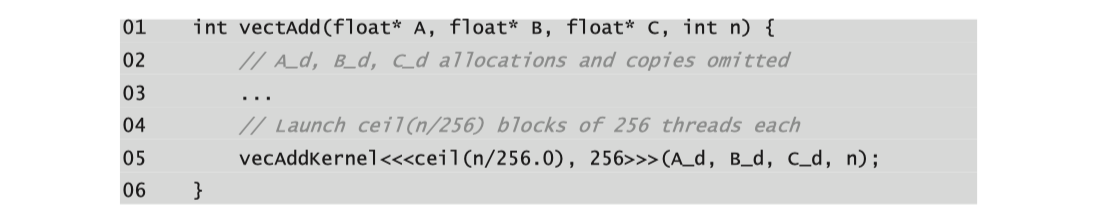
\includegraphics[width=0.9\textwidth]{figs/F2.12.png}
	\caption{\textit{向量加法内核调用语句。}}
\end{figure}

实现内核函数后,剩下的步骤是从主机代码调用该函数来启动网格。 如图 2.12 所示。 当主机代码调用内核时,
它通过执行配置参数设置网格和线程块尺寸。 配置参数在传统 C 函数参数之前的“$<<<$”和“$>>>$”之间给出。 
第一个配置参数给出了网格中的块数。 第二个指定每个块中的线程数。 在此示例中,每个块中有 256 个线程。 
为了确保网格中有足够的线程来覆盖所有向量元素,
我们需要将网格中的块数设置为所需线程数的上限除法(将商四舍五入到直接较高的整数值) 
(本例中为 n)乘以线程块大小(本例中为 256)。 有多种方法可以进行上界划分。 一种方法是将 C 上限函数应用于 n/256.0。 
使用浮点值 256.0 确保我们为除法生成一个浮点值,以便上限值函数可以正确地将其向上舍入。 例如,如果我们想要 1000 个线程,
我们将启动 $ceil(1000/256.0) = 4$ 个线程块。 结果,该语句将启动 $4 \times 256 = 1024$ 个线程。 
通过内核中的 if(i < n) 语句,如图 2.10 所示,前 1000 个线程将对 1000 个向量元素执行加法。 其余 24 个不会。

\begin{figure}[H]
	\centering
	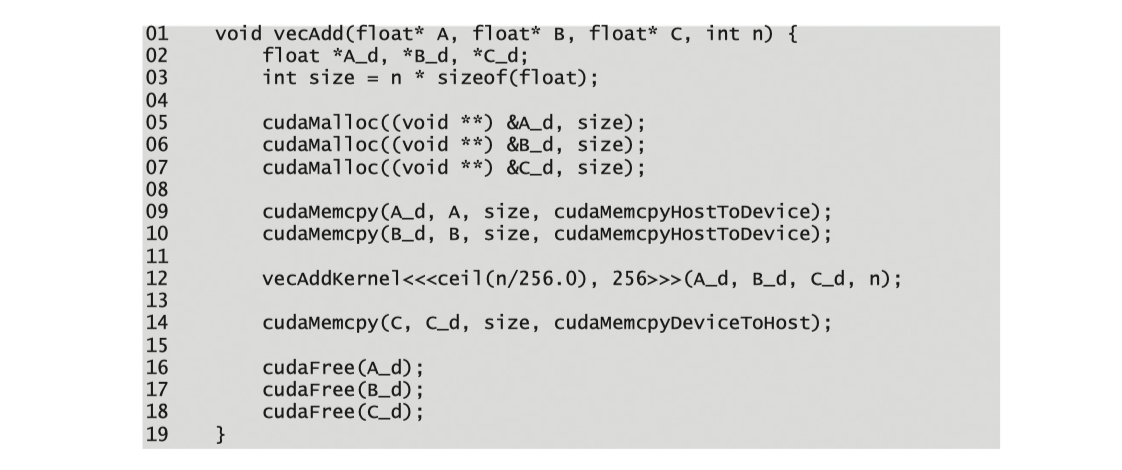
\includegraphics[width=0.9\textwidth]{figs/F2.13.png}
	\caption{\textit{vecAdd 函数中主机代码的完整版本。}}
\end{figure}

图 2.13 显示了 vecAdd 函数中的最终主机代码。 该源代码完成了图 2.5 中的框架。 
2.12和2.13共同说明了一个简单的CUDA程序,它由主机代码和设备内核组成。 该代码被硬连线为使用每个 256 个线程的线程块
\footnote{虽然我们在此示例中使用任意块大小 256,但块大小应由稍后将介绍的许多因素确定。} 。 
但是,所使用的线程块的数量取决于向量 (n) 的长度。 如果n为750,则将使用三个线程块。 如果n为4000,则将使用16个线程块。 
如果n为2,000,000,则将使用7813个块。 请注意,所有线程块都对向量的不同部分进行操作。 
它们可以按任意顺序执行。 程序员不得对执行顺序做出任何假设。 
具有少量执行资源的小型 GPU 可能仅并行执行这些线程块中的一个或两个。 更大的 GPU 可以并行执行 64 或 128 个块。 
这使得 CUDA 内核在硬件执行速度方面具有可扩展性。 
也就是说,相同的代码在小型 GPU 上以较低的速度运行,而在较大的 GPU 上以较高的速度运行。 
我们将在第 4 章“计算架构和调度”中重新讨论这一点。

需要再次指出的是,使用向量加法示例是为了简单起见。 
实际上,分配设备内存、从主机到设备的输入数据传输、
从设备到主机的输出数据传输以及取消分配设备内存的开销可能会使生成的代码比图 2.4 中的原始顺序代码慢。 
这是因为内核完成的计算量相对于处理或传输的数据量来说很小。 对于两个浮点输入操作数和一个浮点输出操作数仅执行一次加法。 
实际应用程序通常具有相对于处理的数据量而言需要更多工作的内核,这使得额外的开销是值得的。 
实际应用程序还倾向于在多个内核调用之间将数据保留在设备内存中,以便可以分摊开销。 我们将展示此类应用的几个示例。

\subsection{编译}
我们已经看到,实现 CUDA C 内核需要使用各种不属于 C 的扩展。一旦在代码中使用了这些扩展,传统的 C 编译器就不再可接受。 
代码需要由能够识别和理解这些扩展的编译器来编译,例如 NVCC(NVIDIA C 编译器)。 
如图2.14顶部所示,NVCC编译器处理CUDA C程序,使用CUDA关键字来分离主机代码和设备代码。 
主机代码是直接的 ANSI C 代码,使用主机的标准 C/C++ 编译器进行编译,并作为传统 CPU 进程运行。 
设备代码标有 CUDA 关键字,指定 CUDA 内核及其关联的辅助函数和数据结构,由 NVCC 编译成称为 PTX 文件的虚拟二进制文件。 
这些 PTX 文件由 NVCC 的运行时组件进一步编译为真实对象文件,并在支持 CUDA 的 GPU 设备上执行。

\begin{figure}[H]
	\centering
	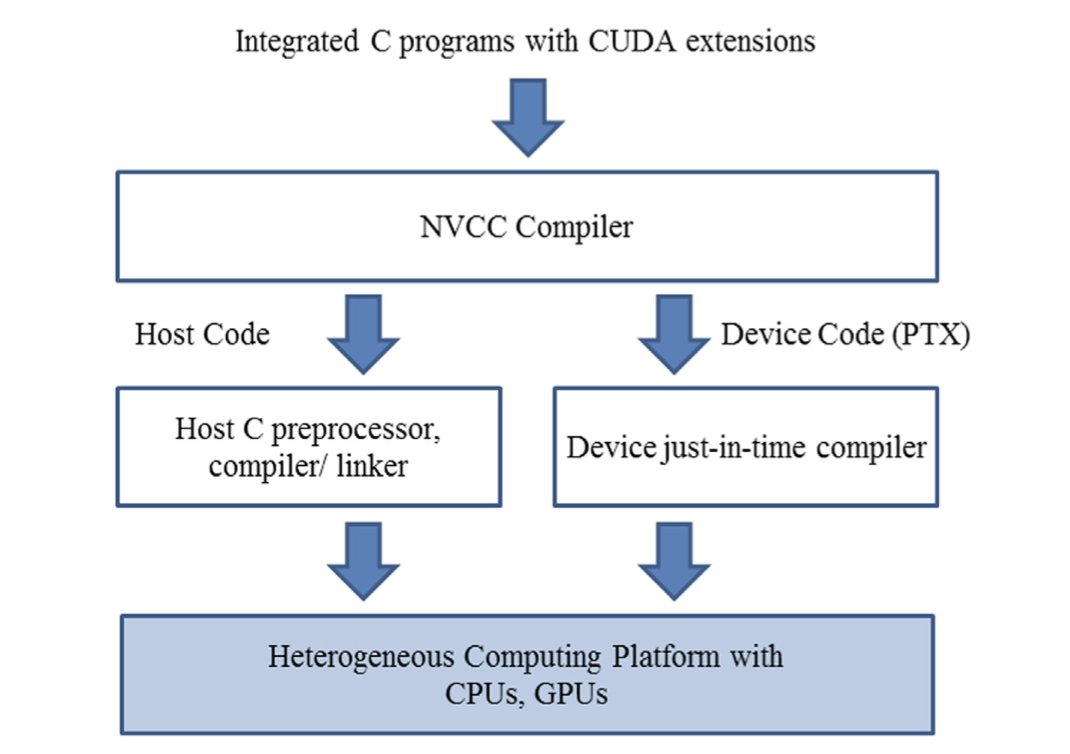
\includegraphics[width=0.9\textwidth]{figs/F2.14.png}
	\caption{\textit{CUDA C 程序的编译过程概述。}}
\end{figure}

\subsection{总结}
本章提供了 CUDA C 编程模型的快速、简化的概述。 CUDA C 扩展了 C 语言以支持并行计算。 
我们在本章中讨论了这些扩展的一个重要子集。 为了您的方便,我们将本章讨论的扩展总结如下:

\subsubsection{函数声明}
CUDA C 扩展了 C 函数声明语法以支持异构并行计算。 图 2.12 总结了这些扩展。 
使用“\_\_global\_\_”、“\_\_device\_\_”或“\_\_host\_\_”之一,
CUDA C 程序员可以指示编译器生成内核函数、设备函数或主机函数。 所有不带任何这些关键字的函数声明都默认为宿主函数。 
如果在函数声明中同时使用“\_\_host\_\_”和“\_\_device\_\_”,编译器会生成该函数的两个版本,
一种用于设备,一种用于主机。 如果函数声明没有任何 CUDA C 扩展关键字,则该函数默认为主机函数。

\subsubsection{核函数调用和网格启动}
CUDA C 使用 $<<<$ 和 $>>>$ 包围的内核执行配置参数扩展了 C 函数调用语法。
这些执行配置参数仅在调用内核函数来启动网格时使用。 
我们讨论了定义网格尺寸和每个块尺寸的执行配置参数。 读者应参阅 CUDA 编程指南(NVIDIA,2021),
了解内核启动扩展以及其他类型的执行配置参数的更多详细信息。


\subsubsection{内置变量}
CUDA 内核可以访问一组内置的、预定义的只读变量,这些变量允许每个线程将自己与其他线程区分开来,并确定要处理的数据区域。 
我们在本章中讨论了 threadIdx、blockDim 和 blockIdx 变量。 
在第 3 章“多维网格和数据”中,我们将讨论使用这些变量的更多细节。

CUDA支持一组API函数来为CUDA C程序提供服务。 我们在本章中讨论的服务是 cudaMalloc、cudaFree 和 cudaMemcpy 函数。 
这些函数由主机代码调用,以分别代表调用程序分配设备全局内存、释放设备全局内存以及在主机和设备之间传输数据。 
读者可参考《CUDA C 编程指南》了解其他 CUDA API 函数。


\subsubsection{运行时应用程序编程接口}
本章的目标是介绍 CUDA C 的核心概念以及用于编写简单的 CUDA C 程序的基本 CUDA C 扩展。 
本章绝不是对所有 CUDA 功能的全面介绍。 其中一些功能将在本书的其余部分中介绍。 
然而,我们的重点将放在这些功能支持的关键并行计算概念上。 我们将仅介绍并行编程技术的代码示例中所需的 CUDA C 功能。 
一般来说,我们鼓励读者始终查阅 CUDA C 编程指南,以了解 CUDA C 功能的更多详细信息。

\newpage
\section{数据管理}
超级计算机架构师经常感叹需要“喂养野兽”。 
“喂养野兽”一词指的是当我们使用大量并行性时我们创建的计算机的“野兽”,并向其提供数据成为需要解决的关键挑战。

在异构机器上提供 SYCL 程序需要小心,以确保数据在需要时位于需要的位置。 
在大型程序中,这可能需要大量工作。 在现有的 C++ 程序中,仅仅弄清楚如何管理所需的所有数据移动就可能是一场噩梦。

我们将仔细解释管理数据的两种方式:统一共享内存(USM)和Buffer。 
USM 是基于指针的,C++ 程序员对此很熟悉。 Buffer提供了更高级别的抽象。 有选择是好的。

我们需要控制数据的移动,本章将介绍实现这一目标的选项。

在第 2 章中,我们研究了如何控制代码的执行位置。 我们的代码需要数据作为输入并生成数据作为输出。 
由于我们的代码可能在多个设备上运行,并且这些设备不一定共享内存,因此我们需要管理数据移动。 
即使数据是共享的(例如使用 USM),同步和一致性也是我们需要理解和管理的概念。

一个合乎逻辑的问题可能是“为什么编译器不自动为我们完成所有事情?” 虽然可以自动为我们处理很多事情,
但如果我们不宣称自己是程序员,那么性能通常不是最佳的。 
在实践中,为了获得最佳性能,我们在编写异构程序时需要关注代码放置(第 2 章)和数据移动(本章)。

本章概述了管理数据,包括控制数据使用的顺序。 它是对前一章的补充,前一章向我们展示了如何控制代码的运行位置。 
本章帮助我们有效地使数据出现在我们要求代码运行的位置,这不仅对于正确执行应用程序很重要,
而且对于最大限度地减少执行时间和功耗也很重要。


\subsection{介绍}
没有数据,计算就毫无意义。 加速计算的全部目的是更快地产生答案。 
这意味着数据并行计算最重要的方面之一是它们如何访问数据,并将加速器设备引入机器使情况进一步复杂化。 
在传统的基于单插槽 CPU 的系统中,我们只有一个内存。 加速器设备通常有自己的附加存储器,无法从主机直接访问。 
因此,支持分立设备的并行编程模型必须提供管理这些多个存储器并在它们之间移动数据的机制。

在本章中,我们概述了数据管理的各种机制。 
我们介绍了统一共享内存和数据管理的Buffer抽象,并描述了内核执行和数据移动之间的关系。

\subsection{数据管理问题}
从历史上看,用于并行编程的共享内存模型的优点之一是它们提供了单一的共享内存视图。 拥有这种单一的内存视图可以简化生活。 
我们不需要做任何特殊的事情来从并行任务访问内存(除了适当的同步以避免数据竞争)。 
虽然某些类型的加速器设备(例如集成 GPU)与主机 CPU 共享内存,但许多离散加速器都有自己的本地内存,
与 CPU 的内存分开,如图 3-1 所示。

{\color{red} Multiple discrete memories }

\subsection{本地设备与远程设备}
在使用直接连接到设备的内存(而不是远程内存)读取和写入数据时,在设备上运行的程序通常性能更好。 
我们将对直接连接的存储器的访问称为本地访问。 对另一台设备内存的访问是远程访问。 
远程访问往往比本地访问慢,因为它们必须通过带宽较低和/或延迟较高的数据链路进行传输。 
这意味着将计算和它将使用的数据放在一起通常是有利的。 
为了实现这一目标,我们必须以某种方式确保数据在不同内存之间复制或迁移,以便将其移至更靠近计算发生的位置。

\subsection{管理多个内存}
管理多个内存大致可以通过两种方式完成:显式地通过我们的程序或隐式地通过 SYCL 运行时库。 
每种方法都有其优点和缺点,我们可以根据情况或个人喜好选择其中一种。

\subsubsection{显式数据移动}
{\color{red} 数据移动和内核执行 }

管理多个存储器的一种选择是在不同存储器之间显式复制数据。 
图 3-2 显示了一个具有离散加速器的系统,我们必须首先将内核所需的任何数据从主机内存复制到加速器内存。 
内核计算结果后,我们必须将这些结果复制回主机,然后主机程序才能使用该数据。

显式数据移动的主要优点是我们可以完全控制数据在不同内存之间传输的时间。 
这很重要,因为重叠计算与数据传输对于在某些硬件上获得最佳性能至关重要。

显式数据移动的缺点是指定所有数据移动可能很乏味且容易出错。 
传输不正确的数据量或不确保在内核开始计算之前已传输所有数据可能会导致不正确的结果。 
从一开始就确保所有数据移动正确可能是一项非常耗时的任务。

\subsubsection{隐式数据}
程序控制的显式数据移动的替代方案是由并行运行时或驱动程序控制的隐式数据移动。 
在这种情况下,并行运行时不需要在不同内存之间进行显式复制,而是负责确保数据在使用之前传输到适当的内存。

隐式数据移动的优点是,应用程序无需花费太多精力即可利用直接连接到设备的更快内存。 
所有繁重的工作都是由运行时自动完成的。 
这也减少了在程序中引入错误的机会,因为运行时将自动识别何时必须执行数据传输以及必须传输多少数据。

隐式数据移动的缺点是我们对运行时隐式机制的行为控制较少或无法控制。 
运行时将提供功能正确性,但可能无法以最佳方式移动数据,以确保计算与数据传输的最大重叠,这可能会对程序性能产生负面影响。

\subsubsection{选择正确的策略}
为项目选择最佳策略可能取决于许多不同的因素。 不同的策略可能适合程序开发的不同阶段。 
我们甚至可以决定最好的解决方案是混合和匹配程序不同部分的显式和隐式方法。 
我们可能会选择开始使用隐式数据移动来简化将应用程序移植到新设备的过程。 
当我们开始调整应用程序的性能时,我们可能会开始在代码的性能关键部分用显式数据移动替换隐式数据移动。 
未来的章节将介绍如何将数据传输与计算重叠以优化性能。

\subsection{USM、Buffer 和 Images}
管理内存有三个抽象:统一共享内存(USM)、Buffer 和 Images。 USM 是一种基于指针的方法,C/C++ 程序员应该熟悉。 
USM 的优点之一是更容易与现有的操作指针的 C++ 代码集成。 Buffer(由Buffer模板类表示)描述一维、二维或三维数组。 
它们提供了可以在主机或设备上访问的内存的抽象视图。 Buffer不由程序直接访问,而是通过访问器对象使用。 
Images充当一种特殊类型的Buffer,提供特定于Images处理的额外功能。 
此功能包括对特殊Images格式的支持、使用采样器对象读取Images等等。 
Buffer和Images是强大的抽象,可以解决许多问题,但重写现有代码中的所有接口以接受Buffer或访问器可能非常耗时。 
由于Buffer和Images的接口基本相同,因此本章的其余部分将仅关注 USM 和Buffer。

\subsection{统一共享内存}
USM 是我们可用于数据管理的一种工具。 
USM 是一种基于指针的方法,使用 malloc 或 new 分配数据的 C 和 C++ 程序员应该熟悉它。 
USM 简化了移植大量使用指针的现有 C/C++ 代码的过程。 支持USM的设备支持统一的虚拟地址空间。 
拥有统一的虚拟地址空间意味着主机上的 USM 分配例程返回的任何指针值都将是设备上的有效指针值。 
我们不必手动转换主机指针来获取“设备版本”——我们在主机和设备上看到相同的指针值。

USM 的更详细描述可以在第 6 章中找到。

\subsubsection{通过指针访问内存}
{\color{red} USM allocation types}

由于当系统同时包含主机内存和一定数量的设备连接本地内存时,并非所有内存都是平等创建的,
因此 USM 定义了三种不同类型的分配:设备、主机和共享。 所有类型的分配都在主机上执行。 
图 3-3 总结了每种分配类型的特征。

设备分配发生在设备附加内存中。 这样的分配可以在设备上读取和写入,但不能从主机直接访问。 
我们必须使用显式复制操作在主机内存中的常规分配和设备分配之间移动数据。

主机分配发生在主机内存中,主机和设备上都可以访问该内存。 这意味着相同的指针值在主机代码和设备内核中都有效。 
然而,当访问这样的指针时,数据总是来自主机存储器。 如果在设备上访问,数据不会从主机迁移到设备本地内存。 
相反,数据通常通过总线发送,例如将设备连接到主机的 PCI Express (PCI-E)。

主机和设备上都可以访问共享分配。 在这方面,它与主机分配非常相似,
但不同之处在于数据现在可以在主机内存和设备本地内存之间迁移。 
这意味着迁移发生后,设备上的访问将从更快的设备本地内存中进行,而不是通过延迟较高的连接远程访问主机内存。 
通常,这是通过运行时内部的机制和对我们隐藏的较低级别驱动程序来完成的。

\subsubsection{USM 和数据移动}
USM 支持显式和隐式数据移动策略,不同的分配类型映射到不同的策略。 
设备分配要求我们在主机和设备之间显式移动数据,而主机和共享分配提供隐式数据移动。

\paragraph{USM 中的显式数据移动}

USM 的显式数据移动是通过设备分配以及队列和 Handler 类中的特殊 memcpy() 来完成的。 
我们将 memcpy() 操作(动作)排入队列,以将数据从主机传输到设备或从设备传输到主机。

{\color{red} USM explicit data movement }

图 3-4 包含一个在设备分配上运行的内核。 在内核使用 memcpy() 操作执行之前和之后,
数据会在 host\_array 和 device\_array 之间复制。 
调用队列上的 wait() 可确保在内核执行之前完成到设备的复制,并确保在数据复制回主机之前内核已完成。 
我们将在本章后面学习如何消除这些调用。

\paragraph{USM 中的隐式数据移动}

USM 的隐式数据移动是通过主机和共享分配来完成的。 
通过这些类型的分配,我们不需要显式插入复制操作来在主机和设备之间移动数据。 
相反,我们只需访问内核内部的指针,任何所需的数据移动都会自动执行,无需程序员干预(只要您的设备支持这些分配)。 
这极大地简化了现有代码的移植:最多我们只需要简单地用适当的 USM 分配函数(以及调用 free 来释放内存)
替换任何 malloc 或 new ,并且一切都应该正常工作。

{\color{red} USM implicit data movement }

在图 3-5 中,我们创建了两个数组:host\_array 和 shared\_array,分别是主机分配和共享分配。 
虽然主机和共享分配都可以在主机代码中直接访问,但我们在这里只初始化 host\_array 。 
同样,可以在内核内部直接访问,进行数据的远程读取。 
运行时确保shared\_array在内核访问它之前在设备上可用,并且当主机代码稍后读取它时将其移回,所有这些都无需程序员干预。

\subsection{Buffer}
为数据管理提供的另一个抽象是 Buffer 对象。 Buffer 是一种数据抽象,表示给定 C++ 类型的一个或多个对象。 
Buffer对象的元素可以是标量数据类型(例如 int、float 或 double)、向量数据类型(第 11 章)或用户定义的类或结构。 
SYCL 2020 定义了一个新概念“设备可复制”,它扩展了可简单复制的概念,并添加了允许类型集。 
特别是,如果常见 C++ 类(例如 std::array、std::pair、std::tuple 或 std::span)中的模板化类型本身是设备可复制的,
那么使用这些类型构建的那些 C++ 类特化也是设备可复制的。 
在将数据类型与Buffer一起使用之前,请注意您的数据类型是设备可复制的!

虽然Buffer本身是单个对象,但Buffer封装的 C++ 类型可以是包含多个对象的数组。 
Buffer代表数据对象而不是特定的内存地址,因此不能像常规 C++ 数组一样直接访问。 
事实上,出于性能原因,Buffer对象可能映射到多个不同设备上的多个不同内存位置,甚至映射到同一设备上。 
相反,我们使用访问器对象来读取和写入Buffer。

Buffer的更详细描述可以在第 7 章中找到。

\subsubsection{创建Buffer}
可以通过多种方式创建Buffer。 最简单的方法是简单地构造一个新的Buffer,其范围指定Buffer的大小。 
然而,以这种方式创建Buffer并不会初始化其数据,这意味着我们必须首先通过其他方式初始化Buffer,
然后才能尝试从中读取有用的数据。

还可以根据主机上的现有数据创建Buffer。 
这是通过调用几个构造函数之一来完成的,这些构造函数采用指向现有主机分配的指针、
一组 InputIterators 或具有某些属性的容器。 在Buffer构造期间,数据从现有主机分配复制到Buffer对象的主机内存中。 
还可以使用 SYCL 互操作性功能(例如,从 OpenCL cl\_mem 对象)从特定于后端的对象创建Buffer。 
有关如何执行此操作的更多详细信息,请参阅有关互操作性的章节。

\subsubsection{访问Buffer}
主机和设备可能无法直接访问Buffer(除非通过此处未描述的高级且不常用的机制)。 
相反,我们必须创建访问器才能读取和写入Buffer。 
访问器为运行时提供有关我们计划如何使用Buffer中的数据的信息,使其能够正确安排数据移动。

\subsubsection{访问模式}
{\color{red} Buffer and accessors }

{\color{red} Buffer access modes}

创建访问器时,我们可以通知运行时我们将如何使用它来提供更多优化信息。 我们通过指定访问模式来做到这一点。 
访问模式在图 3-7 中描述的 access\_mode 枚举类中定义。 
在图 3-6 所示的代码示例中,访问器 my\_accessor 是使用默认访问模式 access\_mode::read\_write 创建的。 
这让运行时知道我们打算通过 my\_accessor 读取和写入Buffer。 访问模式是运行时优化隐式数据移动的方式。 
例如,access\_mode::read 告诉运行时,在该内核开始执行之前,数据需要在设备上可用。 
如果内核仅通过访问器读取数据,则无需在内核完成后将数据复制回主机,因为我们没有修改它。 
同样,access\_mode::write 让运行时知道我们将修改Buffer的内容,并且可能需要在计算结束后将结果复制回来。

使用正确的模式创建访问器可以为运行时提供有关如何在程序中使用数据的更多信息。 
运行时使用访问器来排序数据的使用,但它也可以使用此数据来优化内核的调度和数据移动。 
第 7 章更详细地描述了访问模式和优化标签。

\subsection{对数据的使用进行排序}
内核可以被视为提交执行的异步任务。 这些任务必须提交到队列,并安排它们在设备上执行。 
在许多情况下,内核必须按特定顺序执行,以便计算出正确的结果。 
如果要获得正确结果需要任务 A 先于任务 B 执行,则称任务 A 和任务 B 之间存在依赖关系。
\footnote{请注意,您可能会看到“dependence”和“dependences”有时在其他文本中拼写为“dependency”和“dependencies”。
它们的意思是一样的,但我们倾向于在几篇关于数据流分析的重要论文中使用的拼写。
请参阅 https://dl.acm.org/doi/pdf/10.1145/75277.75280 
和 https:// dl.acm.org/doi/pdf/10.1145/113446.113449。}

然而,内核并不是必须调度的唯一任务形式。 在内核开始执行之前,内核访问的任何数据都需要在设备上可用。 
这些数据依赖性可以以从一个设备到另一设备的数据传输的形式创建额外的任务。 
数据传输任务可以是显式编码的复制操作或更常见的由运行时执行的隐式数据移动。

如果我们获取程序中的所有任务以及它们之间存在的依赖关系,我们可以使用它来将信息可视化为图表。 
该任务图具体来说是有向无环图(DAG),其中节点是任务,边是依赖关系。 
该图是有向的,因为依赖关系是单向的:任务 A 必须在任务 B 之前发生。该图是非循环的,
因为它不能包含从节点返回到自身的任何循环或路径。

{\color{red} 简单的任务图 }

在图 3-8 中,任务 A 必须在任务 B 和 C 之前执行。同样,B 和 C 必须在任务 D 之前执行。
由于 B 和 C 之间没有依赖关系,因此运行时可以自由地以任何顺序执行它们 (甚至并行)只要任务 A 已经执行。 
因此,该图可能的合法顺序是 A $\rightarrow$ B $\rightarrow$ C $\rightarrow$ D、
A $\rightarrow$ C $\rightarrow$ B $\rightarrow$ D,如果 B 和 C 可以同时执行,
甚至是 A $\rightarrow$ \{B,C\} $\rightarrow$ D。

{\color{red} 具有不相交依赖关系的任务图}

任务可能与所有任务的子集具有依赖性。 在这些情况下,我们只想指定对正确性重要的依赖关系。 
这种灵活性为运行时提供了优化任务图执行顺序的自由度。 
在图 3-9 中,我们扩展了图 3-8 中的早期任务图,添加了任务 E 和 F,其中 E 必须在 F 之前执行。
但是,任务 E 和 F 与节点 A、B、C 和 D 没有依赖关系。 这允许运行时从许多可能的合法顺序中进行选择来执行所有任务。

有两种不同的方法来对队列中任务的执行(例如启动内核)进行建模:队列可以按照提交的顺序执行任务,
也可以按照我们指定的任何依赖项的任何顺序执行任务。 我们可以通过多种机制来定义正确排序所需的依赖关系。

\subsubsection{有序队列}
{\color{red} In-order queue usage}

对任务进行排序的最简单选项是将它们提交到有序队列对象。 有序队列按照任务提交的顺序执行任务,如图 3-10 所示。 
它们直观的任务排序意味着有序队列具有简单性的优点,但具有序列化任务的缺点,即使独立任务之间不存在依赖性。 
有序队列在启动应用程序时非常有用,因为它们简单、直观、执行顺序确定,并且适合许多代码。

\subsubsection{无序队列}
由于队列对象是无序队列(除非使用 inorder 队列属性创建),因此它们必须提供对提交给它们的任务进行排序的方法。 
队列通过让我们通知运行时任务之间的依赖关系来对任务进行排序。 可以使用命令组显式或隐式地指定这些依赖性。 
我们将在以下部分中分别考虑它们。

命令组是指定任务及其依赖性的对象。 命令组通常编写为 C++ lambda 表达式,作为参数传递给队列对象的 Submit() 方法。 
该 lambda 的唯一参数是对Handler对象的引用。 Handler对象在命令组内部使用来指定操作、创建访问器并指定依赖关系。

\paragraph{与事件的显式依赖关系}

任务之间的显式依赖关系类似于我们看到的示例(图 3-8),其中任务 A 必须在任务 B 之前执行。
以这种方式表达依赖关系侧重于基于发生的计算而不是计算访问的数据的显式排序 。 
请注意,表达计算之间的依赖关系主要与使用 USM 的代码相关,因为使用Buffer的代码通过访问器表达大多数依赖关系。 
在图 3-4 和 3-5 中,我们只是告诉队列等待所有先前提交的任务完成,然后再继续。 
相反,我们可以通过事件对象来表达任务依赖性。 将命令组提交到队列时,submit() 方法返回一个事件对象。 
这些事件可以通过两种方式使用。

首先,我们可以通过显式调用事件的 wait() 方法来通过主机进行同步。 
这会强制运行时等待生成事件的任务完成执行,然后主机程序才能继续执行。 
显式等待事件对于调试应用程序非常有用,但 wait() 可能会过度限制任务的异步执行,因为它会停止主机线程上的所有执行。 
类似地,我们还可以对队列对象调用 wait(),这将阻止主机上的执行,直到所有排队的任务完成为止。 
如果我们不想跟踪排队任务返回的所有事件,这可能是一个有用的工具。

这给我们带来了使用事件的第二种方式。 Handler类包含一个名为depends\_on() 的方法。 
此方法接受单个事件或事件向量,并通知运行时正在提交的命令组需要完成指定的事件,然后才能执行命令组内的操作。 
图 3-11 显示了如何使用 dependent\_on() 来排序任务的示例。

{\color{red} Using events and depends\_on}

\paragraph{与访问器的隐式依赖关系}

{\color{red} Three forms of data dependences}

任务之间的隐式依赖关系是根据数据依赖关系创建的。 任务之间的数据依赖关系有三种形式,如图 3-12 所示。

{\color{red} Read-after-Write}

{\color{red} RAW task graph}

数据依赖性以两种方式表达给运行时:访问器和程序顺序。 运行时必须使用两者来正确计算数据依赖性。 
图 3-13 和 3-14 对此进行了说明。

在图 3-13 和 3-14 中,我们执行三个内核——computeB、readA 和computeC——然后在主机上读回最终结果。 
内核computeB的命令组创建两个访问器a和b。 这些访问器使用访问标记 read\_only 和 write\_only 进行优化,
以指定我们不使用默认访问模式 access\_mode::read\_write。 我们将在第 7 章中了解有关访问标记的更多信息。
内核computeB 读取 Buffer a\_buf 并写入 Buffer b\_buf。 
在内核开始执行之前,必须将 Buffer a\_buf 从主机复制到设备。

内核 readA 还为Buffer a\_buf 创建一个只读访问器。 
由于内核 readA 是在内核computeB 之后提交的,因此这会创建 Read-afterRead (RAR) 场景。 
然而,RAR 不会对运行时施加额外的限制,并且内核可以自由地以任何顺序执行。 
事实上,运行时可能更喜欢在内核computeB之前执行内核readA,甚至同时执行两者。 
两者都需要将Buffer a\_buf 复制到设备,但内核computeB还需要复制Buffer b\_buf,
以防任何现有值不被 computeB 覆盖并且可能被以后的内核使用。 
这意味着运行时可以在Buffer b\_buf 的数据传输发生时执行内核 readA,并且还表明即使内核仅写入Buffer,
Buffer的原始内容仍可能被移动到设备,
因为无法保证 Buffer中的所有值都将由内核写入(请参阅第 7 章了解允许我们在这些情况下进行优化的标签)。

内核computeC读取Buffer b\_buf,这是我们在内核computeB中计算的。 
由于我们在提交内核computeB之后提交了内核computeC,这意味着内核computeC对Buffer b\_buf 有RAW数据依赖。 
RAW 依赖关系也称为真实依赖关系或流依赖关系,因为数据需要从一个计算流到另一个计算才能计算出正确的结果。 
最后,我们还在内核computeC和主机之间创建对Buffer c\_buf 的RAW依赖,因为主机希望在内核完成后读取C。 
这会强制运行时将Buffer c\_buf 复制回主机。 
由于设备上没有对Buffer a\_buf 进行写入,因此运行时不需要将该Buffer复制回主机,因为主机已经拥有最新的副本。

{\color{red} Write-after-Read and Write-after-Write}

{\color{red} WAR and WAW task graph}

在图 3-15 和 3-16 中,我们再次执行三个内核:computeB、rewriteA 和 rewriteB。 
内核computeB再次读取Buffer a\_buf 并写入Buffer b\_buf,
内核rewriteA写入Buffer a\_buf,内核rewriteB写入Buffer b\_buf。 
理论上,内核 rewriteA 可以比内核computeB 更早执行,因为在内核准备好之前需要传输的数据较少,
但它必须等到内核computeB 完成之后,因为对Buffer a\_buf 存在WAR 依赖性。

在这个例子中,内核computeB需要来自主机的A的原始值,如果内核rewriteA在内核computeB之前执行,它将读取错误的值。 
WAR 依赖也称为反依赖。 RAW 依赖性确保数据正确地流向正确的方向,而 WAR 依赖性确保现有值在读取之前不会被覆盖。 
WAW 对Buffer b\_buf 的依赖在内核重写函数中也类似。 
如果在内核computeB和rewriteB之间提交了对Buffer b\_buf 的任何读取,它们将导致RAW和WAR依赖性,从而正确排序任务。 
然而,在此示例中,内核 rewriteB 和主机之间存在隐式依赖性,因为最终数据必须写回主机。 
我们将在第 7 章中详细了解导致此写回的原因。WAW 依赖性,也称为输出依赖性,可确保最终输出在主机上正确。

\subsection{选择数据管理策略}
为我们的应用程序选择正确的数据管理策略很大程度上取决于个人喜好。 
事实上,我们可能会从一种策略开始,随着我们的项目成熟而转向另一种策略。 
然而,有一些有用的指南可以帮助我们选择满足我们需求的策略。

首先要做的决定是我们是否要使用显式或隐式数据移动,因为这极大地影响了我们需要对程序执行的操作。 
隐式数据移动通常是一个更容易开始的地方,因为所有数据移动都为我们处理,让我们专注于计算的表达。

如果我们决定从一开始就完全控制所有数据移动,那么我们要从使用 USM 设备分配的显式数据移动开始。 
我们只需要确保在主机和设备之间添加所有必要的副本即可!

当选择隐式数据移动策略时,我们仍然可以选择是使用Buffer还是USM主机或共享指针。 
同样,这种选择取决于个人喜好,但有几个问题可以帮助我们选择其中一个。 
如果我们要移植使用指针的现有 C/C++ 程序,USM 可能是一条更简单的路径,因为大多数代码不需要更改。 
如果数据表示没有引导我们做出偏好,我们可以问的另一个问题是我们希望如何表达内核之间的依赖关系。 
如果我们更愿意考虑内核之间的数据依赖性,请选择Buffer。 
如果我们更愿意将依赖关系视为在另一项计算之前执行一项计算,
并希望使用有序队列或显式事件或内核之间的等待来表达这一点,请选择 USM。

当使用 USM 指针(显式或隐式数据移动)时,我们可以选择要使用哪种类型的队列。 
有序队列简单直观,但它们限制了运行时间并可能限制性能。 
无序队列更复杂,但它们为运行时提供了更大的自由度来重新排序和重叠执行。 
如果我们的程序在内核之间具有复杂的依赖关系,那么无序队列类是正确的选择。 
如果我们的程序只是一个接一个地运行许多内核,那么有序队列对我们来说将是一个更好的选择。

\subsection{Handler类:关键成员}
{\color{red} Simplified definition of the non-accessor members of the handler class}

{\color{red} Simplified definition of the accessor members of the handler class}

我们已经展示了多种使用Handler类的方法。 图 3-17 和 3-18 提供了这个非常重要的类的关键成员的更详细的解释。 
我们还没有使用所有这些成员,但稍后将在本书中使用它们。 这是放置它们的好地方。

一个密切相关的类,队列类,在第 2 章末尾有类似的解释。

\subsection{概括}
在本章中,我们介绍了解决数据管理问题的机制以及如何排序数据的使用。 
使用加速器设备时,管理对不同内存的访问是一个关键挑战,我们有不同的选项来满足我们的需求。

我们概述了数据使用之间可能存在的不同类型的依赖关系,
并描述了如何向队列提供有关这些依赖关系的信息,以便它们正确排序任务。

本章概述了统一共享内存和Buffer。 我们在第 6 章中更详细地探讨了 USM 的所有模式和行为。
第 7 章更深入地探讨了Buffer,包括创建Buffer和控制其行为的所有不同方法。 
第 8 章回顾了控制内核执行和数据移动顺序的队列调度机制。

\newpage
\section{计算架构和调度}
在第 1 章“简介”中,我们看到 CPU 的设计目的是最大限度地减少指令执行的延迟,
而 GPU 的设计目的是最大限度地提高执行指令的吞吐量。 在第 2 章“异构数据并行计算”和第 3 章“多维网格和数据”中,
我们学习了 CUDA 编程接口的核心功能,用于创建和调用内核来启动和执行线程。 
在接下来的三章中,我们将讨论现代 GPU 的架构,包括计算架构和内存架构,以及源于对这种架构的理解的性能优化技术。 
本章介绍了 GPU 计算架构的几个方面,这些方面对于 CUDA C 程序员理解和推理其内核代码的性能行为至关重要。 
我们将首先展示计算架构的高级简化视图,并探讨灵活的资源分配、块调度和占用的概念。 
然后我们将深入讨论线程调度、延迟容忍、控制发散和同步。 
我们将通过描述可用于查询 GPU 中可用资源的 API 函数以及在执行内核时帮助估计 GPU 占用率的工具来结束本章。 
在接下来的两章中,我们将介绍GPU内存架构的核心概念和编程注意事项。 
特别是,第 5 章“内存架构和数据局部性”重点介绍了片上内存架构,第 6 章“性能考虑因素”简要介绍了片外内存架构,
然后详细阐述了整个 GPU 架构的各种性能考虑因素。 掌握这些概念的 CUDA C 程序员能够很好地编写和理解高性能并行内核。

\subsection{现代GPU架构}
\begin{figure}[H]
	\centering
	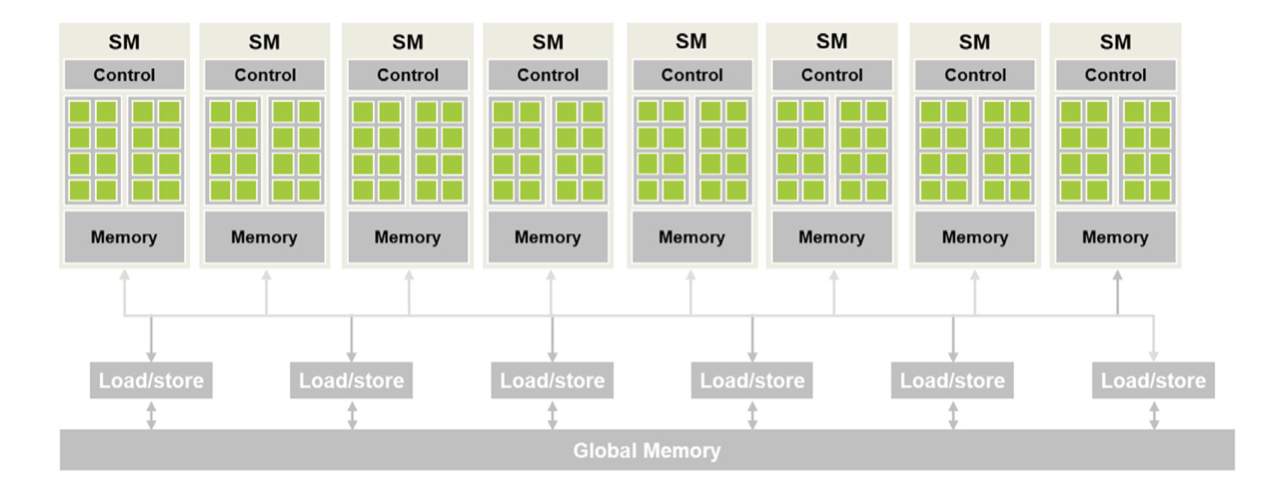
\includegraphics[width=0.9\textwidth]{figs/F4.1.png}
	\caption{\textit{支持 CUDA 的 GPU 架构。}}
\end{figure}

图 4.1 显示了 CUDA C 程序员对典型支持 CUDA 的 GPU 架构的高级视图。 它被组织成一系列高度线程化的流式多处理器(SM)。 
每个 SM 都有多个称为流处理器或 CUDA 核心(以下简称为核心)的处理单元,如图 4.1 中 SM 内的小块所示,
它们共享控制逻辑和内存资源。 例如,Ampere A100 GPU有108个SM,每个SM有64个核心,整个GPU总共有6912个核心。

SM 还具有不同的片上存储器结构,在图 4.1 中统称为“存储器”。 这些片上存储器结构将是第 5 章“存储器架构和数据局部性”的主题。 
GPU 还配备了千兆字节的片外设备内存,在图 4.1 中称为“全局内存”。 虽然较旧的 GPU 使用图形双数据速率同步 DRAM,
但从 NVIDIA Pascal 架构开始的较新 GPU 可能会使用 HBM(高带宽内存)或 HBM2,
它们由与 GPU 紧密集成在同一封装中的 DRAM(动态随机存取存储器)模块组成。 为了简洁起见,在本书的其余部分中,
我们将所有这些类型的内存广泛地称为 DRAM。 我们将在第 6 章“性能注意事项”中讨论访问 GPU DRAM 所涉及的最重要概念。

\subsection{Block 调度}
当调用内核时,CUDA 运行时系统会启动执行内核代码的线程网格。 这些线程逐块分配给 SM。 
也就是说,一个块中的所有线程同时分配给同一个SM。

\begin{figure}[H]
	\centering
	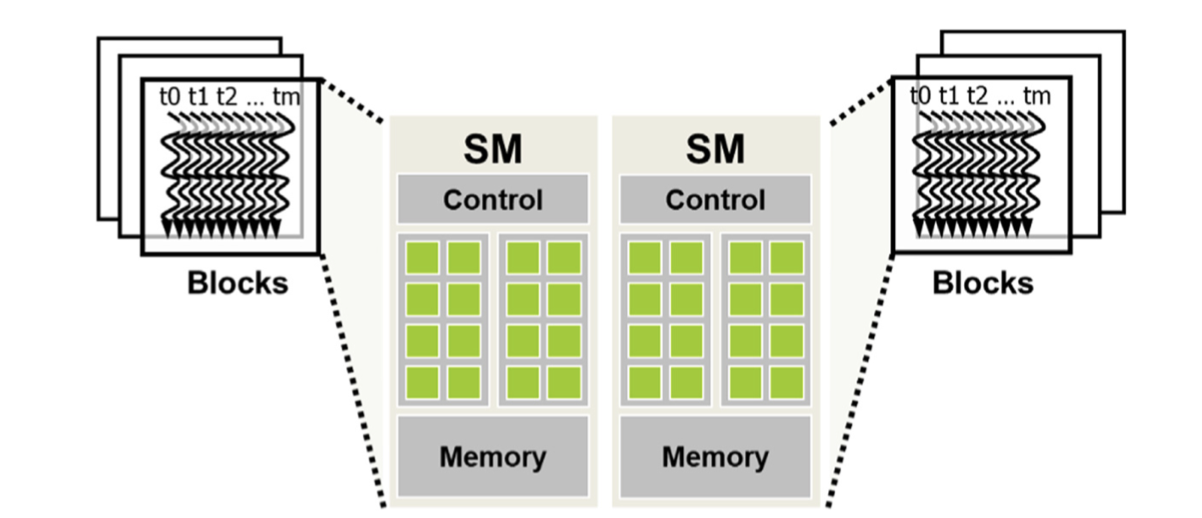
\includegraphics[width=0.9\textwidth]{figs/F4.2.png}
	\caption{\textit{流式多处理器 (SM) 的线程块分配。}}
\end{figure}

图 4.2 说明了块到 SM 的分配。 多个块可能同时分配给同一个 SM。 例如,在图4.2中,每个SM分配了三个块。 
然而,块需要预留硬件资源来执行,因此只能将有限数量的块同时分配给给定的SM。 块数量的限制取决于第 4.6 节中讨论的各种因素。

由于 SM 数量有限以及可以同时分配给每个 SM 的块数量有限,因此可以在 CUDA 设备中同时执行的块总数受到限制。 
大多数网格包含的块比这个数量多得多。 为了确保网格中的所有块都得到执行,运行时系统维护需要执行的块的列表,
并在先前分配的块完成执行时将新块分配给SM。

以块为单位将线程分配给SM可以保证同一块中的线程在同一SM上同时调度。 
这种保证使得同一块中的线程可以以跨不同块的线程无法进行的方式相互交互
\footnote{不同块中的线程可以通过Cooperative Groups API进行屏障同步。 
然而,必须遵守几个重要的限制,以确保涉及的所有线程确实在 SM 上同时执行。 
有兴趣的读者可以参阅《CUDA C 编程指南》以正确使用 Cooperative Groups API。} 。
这包括屏障同步,这将在 4.3 节中讨论。 
它还包括访问驻留在 SM 上的低延迟共享内存,这将在第 5 章“内存架构和数据局部性”中讨论。

\subsection{同步和透明的规模化}
CUDA 允许同一块中的线程使用屏障同步函数 \_\_syncthreads() 协调其活动。 请注意,“\_\_”由两个“\_”字符组成。 
当线程调用 \_\_syncthreads() 时,它将保留在调用的程序位置,直到同一块中的每个线程都到达该位置。 
这确保了块中的所有线程都已完成其执行的一个阶段,然后它们中的任何一个都可以进入下一阶段。

屏障同步是协调并行活动的一种简单且流行的方法。 在现实生活中,我们经常使用屏障同步来协调多人的并行活动。 
例如,假设四个朋友开车去购物中心。 他们都可以去不同的商店购买自己的衣服。 这是一项并行活动,
并且比他们全部作为一个组并依次访问所有感兴趣的商店的情况要高效得多。 然而,在他们离开商场之前,需要进行屏障同步。 
他们必须等到四个朋友都回到车上后才能离开。 比其他人早完成的人必须等待比其他人更晚完成的人。 
如果没有障碍同步,当汽车离开时,一个或多个人可能会留在商场里,这可能会严重损害他们的友谊!

\begin{figure}[H]
	\centering
	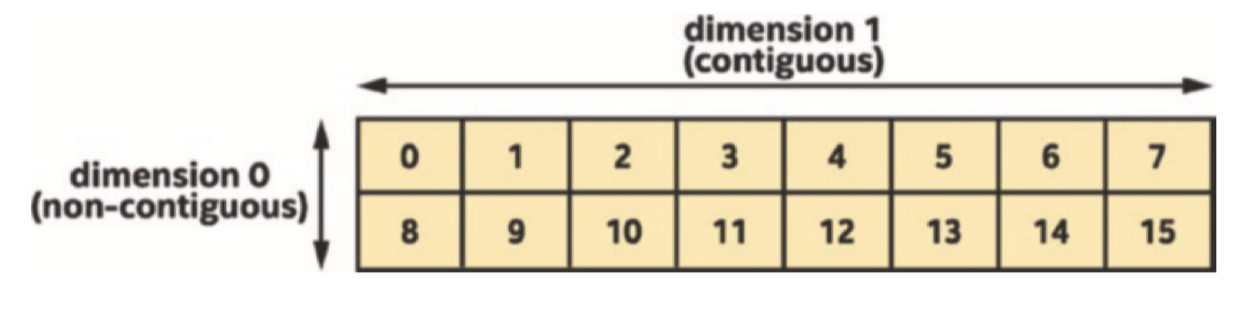
\includegraphics[width=0.9\textwidth]{figs/F4.3.png}
	\caption{\textit{屏障同步的执行示例。 箭头代表一段时间内的执行活动。 
	垂直曲线标记每个线程执行\_\_syncthreads语句的时间。 
	垂直曲线右侧的空白区域描述了每个线程等待所有线程完成的时间。 
	竖线标记最后一个线程执行\_\_syncthreads语句的时间,
	之后所有线程都可以继续执行\_\_syncthreads语句之后的语句。}}
\end{figure}

图 4.3 说明了屏障同步的执行过程。 块中有N个线程。 时间从左向右。 有些线程较早到达屏障同步语句,有些则晚得多。 
早到的人会等待迟到的人。 当最新的线程到达屏障时,所有线程都可以继续执行。 通过屏障同步,“没有人被抛在后面”。

\begin{figure}[H]
	\centering
	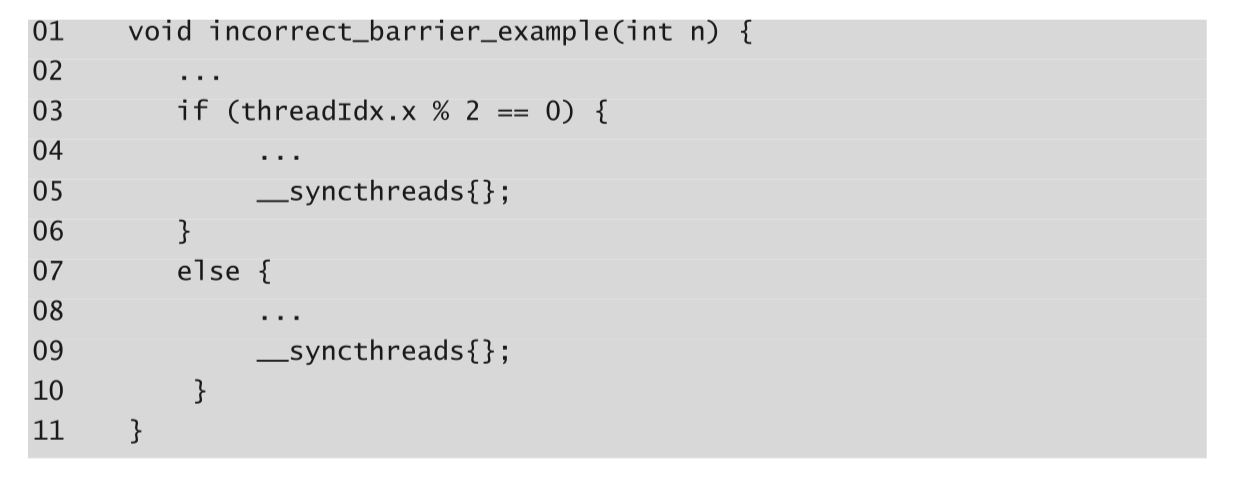
\includegraphics[width=0.9\textwidth]{figs/F4.4.png}
	\caption{\textit{\_\_syncthreads() 的错误使用}}
\end{figure}

在 CUDA 中,如果存在 \_\_syncthreads() 语句,则它必须由块中的所有线程执行。 
当 \_\_syncthreads() 语句放置在 if 语句中时,块中的所有线程要么执行包含 \_\_syncthreads() 的路径,要么都不执行。 
对于 if-then-else 语句,如果每个路径都有 \_\_syncthreads() 语句,则块中的所有线程要么执行 then-path,
要么全部执行 else-path。 两个\_\_syncthreads()是不同的屏障同步点。 
例如,在图 4.4 中,从第 04 行开始的 if 语句中使用了两个 \_\_syncthreads()。
所有具有偶数 threadIdx.x 值的线程都执行 then 路径,而其余线程则执行 else 路径。 
第 06 行和第 10 行的 \_\_syncthreads() 调用定义了两个不同的屏障。 由于并非块中的所有线程都保证执行任一屏障,
因此代码违反了使用 \_\_syncthreads() 的规则,并将导致未定义的执行行为。 
一般来说,不正确地使用屏障同步可能会导致不正确的结果,或者导致线程永远相互等待,这称为死锁。 
程序员有责任避免这种不恰当地使用屏障同步。

屏障同步对块内的线程施加执行约束。 这些线程应在彼此接近的时间执行,以避免等待时间过长。 
更重要的是,系统需要确保参与屏障同步的所有线程都可以访问最终到达屏障所需的资源。 
否则,永远不会到达屏障同步点的线程可能会导致死锁。 
CUDA 运行时系统通过将执行资源分配给块中的所有线程作为一个单元来满足此约束,如我们在 4.2 节中看到的。 
块中的所有线程不仅必须分配给同一个 SM,而且还需要同时分配给该 SM。 
也就是说,只有当运行时系统获得了块中所有线程完成执行所需的所有资源时,块才能开始执行。 
这确保了块中所有线程的时间接近性,并防止屏障同步期间出现过多甚至不确定的等待时间。

\begin{figure}[H]
	\centering
	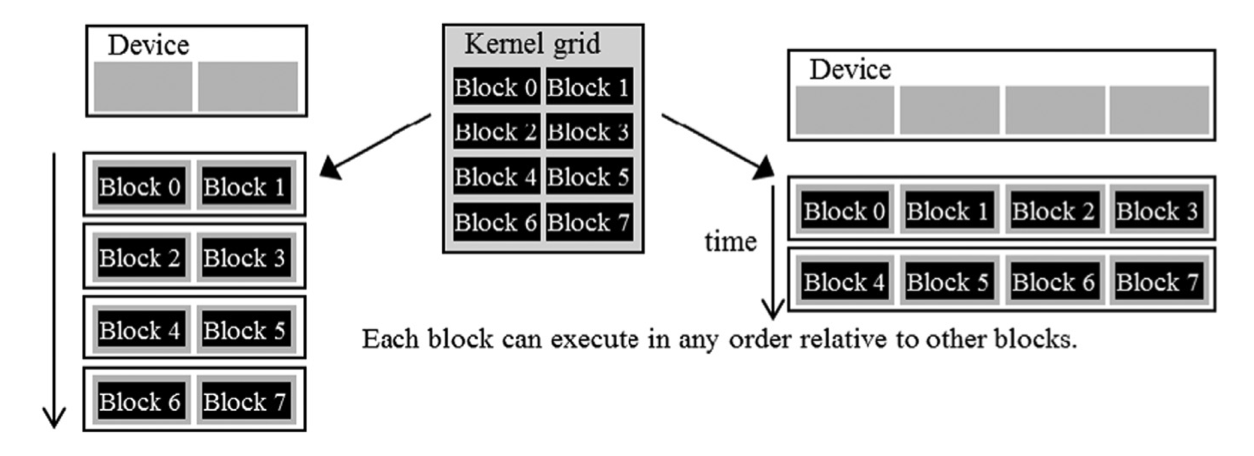
\includegraphics[width=0.9\textwidth]{figs/F4.5.png}
	\caption{\textit{块之间缺乏同步约束使得 CUDA 程序具有透明的可扩展性。}}
\end{figure}

这导致我们在 CUDA 屏障同步设计中进行重要的权衡。 通过不允许不同块中的线程彼此执行屏障同步,
CUDA 运行时系统可以以相对于彼此的任何顺序执行块,因为它们都不需要彼此等待。 这种灵活性支持可扩展的实施,
如图 4.5 所示。 图中时间从上到下依次进行。 在只有少量执行资源的低成本系统中,可以同时执行少量块,如图 4.5 左侧所示,
一次执行两个块。 在具有更多执行资源的高端实现中,可以同时执行许多块,如图 4.5 右侧所示,一次执行四个块。 
如今的高端 GPU 可以同时执行数百个块。

以多种速度执行相同应用程序代码的能力允许根据不同细分市场的成本、功耗和性能要求生产多种实施方案。 
例如,移动处理器可以缓慢但以极低的功耗执行应用程序,而桌面处理器可以以更高的速度执行相同的应用程序但消耗更多的功率。 
两者都执行相同的应用程序,无需更改代码。 
在不同的硬件上以不同数量的执行资源执行相同的应用程序代码的能力被称为透明的可扩展性,
它减轻了应用程序开发人员的负担并提高了应用程序的可用性。

\subsection{warp和 SIMD 硬件}
我们已经看到,块可以按照彼此相对的任何顺序执行,这允许跨不同设备的透明可扩展性。 
然而,我们并没有过多谈论每个块内线程的执行时序。 从概念上讲,应该假设块中的线程可以按彼此之间的任何顺序执行。 
在具有阶段的算法中,每当我们想要确保所有线程在任何线程开始下一阶段之前都已完成其执行的前一阶段时,就应该使用屏障同步。 
执行内核的正确性不应依赖于某些线程将在不使用屏障同步的情况下彼此同步执行的假设。

CUDA GPU 中的线程调度是一个硬件实现概念,因此必须在特定硬件实现的背景下进行讨论。 在迄今为止的大多数实现中,
一旦将块分配给 SM,它就会被进一步划分为称为线程束(warp)的 32 线程单元。 warp的大小是特定于实现的,
并且在未来几代 GPU 中可能会有所不同。 了解warp有助于理解和优化特定代 CUDA 设备上的 CUDA 应用程序的性能。

\begin{figure}[H]
	\centering
	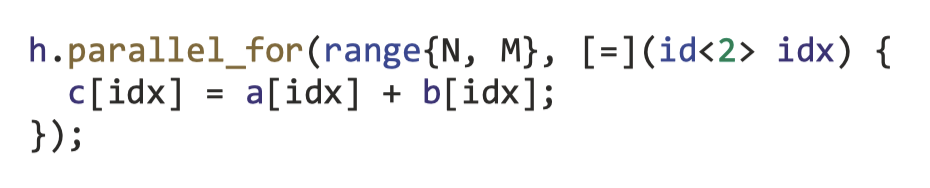
\includegraphics[width=0.9\textwidth]{figs/F4.6.png}
	\caption{\textit{块被划分为线程束以进行线程调度。}}
\end{figure}

Warp是SM中线程调度的单位。 图 4.6 显示了实现中将块划分为 warp 的情况。 
在此示例中,存在三个块:块 1、块 2 和块 3 — 全部分配给 SM。 出于调度目的,这三个块中的每一个都被进一步划分为 warp。 
每个 warp 由 32 个具有连续 threadIdx 值的线程组成:线程 0 到 31 形成第一个 warp,线程 32 到 63 形成第二个 warp,
依此类推。 我们可以计算给定块大小和分配给每个 SM 的给定块数的 SM 中驻留的warp数量。 
在这个例子中,如果每个块有256个线程,我们可以确定每个块有256/32或8个warp。 
SM 中有 3 个块,SM 中有 $8 \times 3 = 24$ 个warp。 根据线程索引将块划分为warp。 
如果将一个块组织成一维数组,即只使用threadIdx.x,那么分区就很简单了。 warp 内的 threadIdx.x 值是连续的并且递增。 
对于warp尺寸 32,warp 0 从线程 0 开始,以线程 31 结束,warp 1 从线程 32 开始,以线程 63 结束,依此类推。 
一般来说,warp n 以线程 $32 \times n$ 开始,以线程 $32 \times (n+1) - 1$ 结束。对于大小不是 32 倍数的块,
最后一个 warp 将用不活动的线程填充,以填充 32 个线程位置。 
例如,如果一个块有 48 个线程,它将被划分为两个 warp,第二个 warp 将填充 16 个不活动线程。

对于由多个维度的线程组成的块,在划分为warp之前,维度将被投影到线性化的行主布局中。 
线性布局是通过将 y 和 z 坐标较大的行放置在较小的行之后来确定的。 
也就是说,如果一个块由二维线程组成,则将所有threadIdx.y为1的线程放置在threadIdx.y为0的线程之后,形成线性布局。
threadIdx.y为2的线程将放置在threadIdx.y为2的线程之后。 其threadIdx.y为1,依此类推。 
具有相同 threadIdx.y 值的线程按 threadIdx.x 递增顺序放置在连续位置。

\begin{figure}[H]
	\centering
	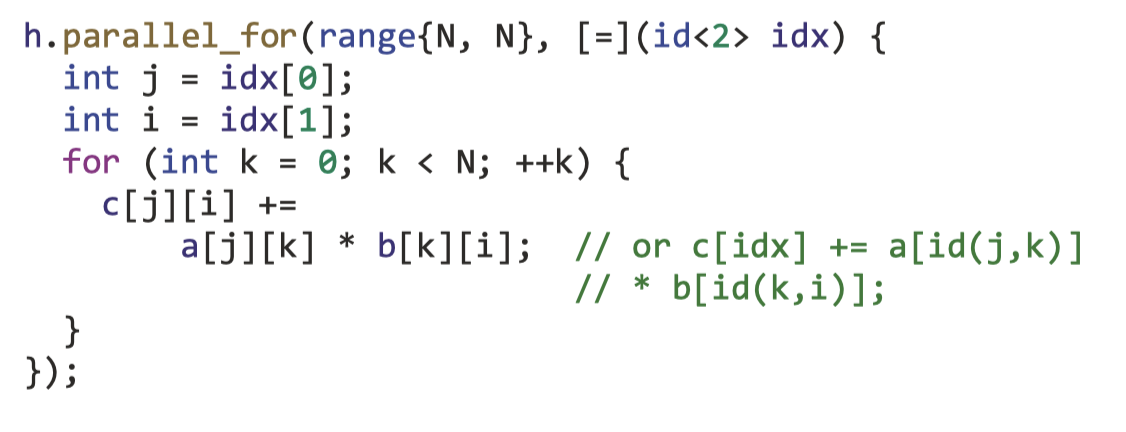
\includegraphics[width=0.9\textwidth]{figs/F4.7.png}
	\caption{\textit{将 2D 线程放置到线性布局中。}}
\end{figure}

图 4.7 显示了将二维块的线程放入线性布局的示例。 上半部分显示了块的二维视图。 
读者应该认识到与二维数组的行优先布局的相似性。 每个线程显示为 $T_{y,x}$ ,x 为 threadIdx.x,y 为 threadIdx.y。 
图 4.7 的下半部分显示了该块的线性化视图。 前4个线程是threadIdx.y值为0的线程; 它们按照递增的 threadIdx.x 值排序。 
接下来的四个线程是 threadIdx.y 值为 1 的线程。它们也以递增的 threadIdx.x 值放置。 
在此示例中,所有 16 个线程形成半个warp。 warp将用另外 16 个线程填充,以完成 32 线程的warp。 
想象一个具有 $8 \times 8$ 个线程的二维块。 64 个线程将形成两个 warp。 
第一个warp从 $T_{0,0}$ 开始,以 $T_{3,7}$ 结束。 
第二个warp从 $T_{4,0}$ 开始,到 $T_{7,7}$ 结束。 对于读者来说,画出这幅画作为练习是很有用的。

对于三维块,我们首先将所有threadIdx.z值为0的线程放入线性顺序。 这些线程被视为一个二维块,如图 4.7 所示。 
所有 threadIdx.z 值为 1 的线程将被放入线性顺序中,依此类推。 
例如,对于三维 2 x 8 x 4 块(x 维度 4 个,y 维度 8 个,z 维度 2 个),
64 个线程将被划分为两个 warp,其中 $T_{0,0}$, 
第一个warp中为 0 到 $T_{0,7,3}$,第二个warp中为 $T_{1,0,0}$ 到 $T_{1,7,3}$。

\begin{figure}[H]
	\centering
	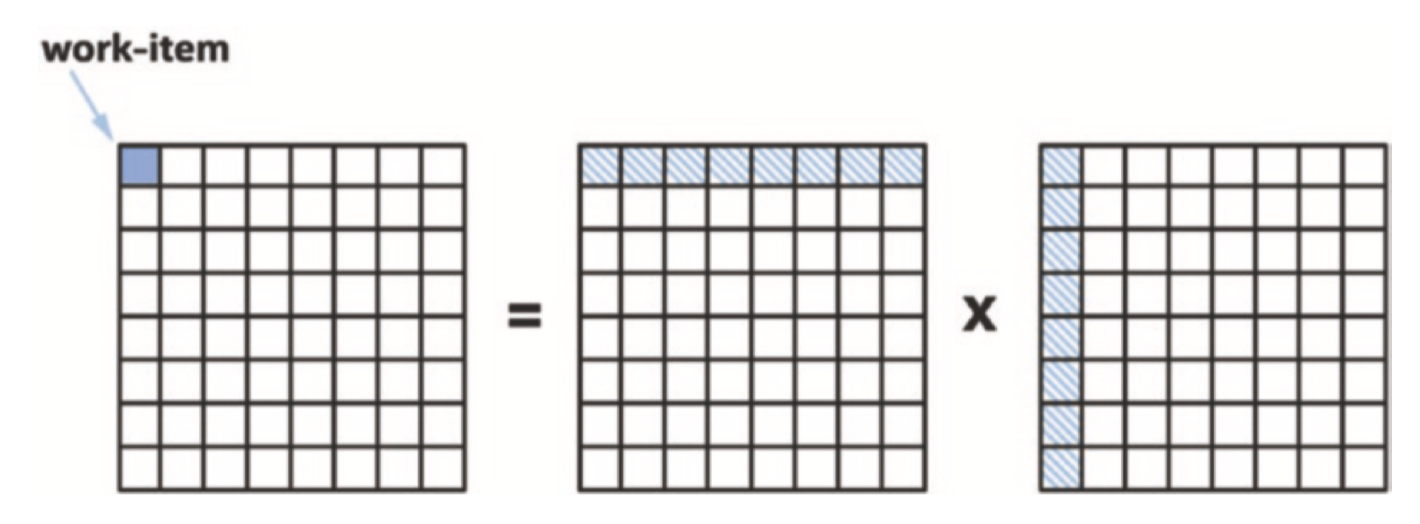
\includegraphics[width=0.9\textwidth]{figs/F4.8.png}
	\caption{\textit{流式多处理器被组织成用于 SIMD 执行的处理块。}}
\end{figure}

SM 旨在按照单指令、多数据 (SIMD) 模型执行 warp 中的所有线程。 也就是说,在任何时刻,
都会为 warp 中的所有线程获取并执行一条指令(请参阅“Warps 和 SIMD 硬件”侧边栏)。 
图 4.8 显示了 SM 中的核心如何分组为处理块,其中每 8 个核心形成一个处理块并共享一个指令获取/调度单元。 
作为一个真实的例子,Ampere A100 SM 有 64 个核心,被组织成四个处理块,每个处理块有 16 个核心。 
同一 warp 中的线程被分配到同一个处理块,该处理块获取该 warp 的指令并同时为该 warp 中的所有线程执行该指令。 
这些线程将相同的指令应用于数据的不同部分。 由于SIMD硬件有效地限制了warp中的所有线程在任何时间点执行相同的指令,
所以warp的执行行为通常被称为单指令、多线程。

SIMD 的优点是控制硬件(例如指令获取/调度单元)的成本由许多执行单元共享。 这种设计选择允许较小比例的硬件专用于控制,
而较大比例的硬件专用于提高算术吞吐量。 我们预计在可预见的将来,warp分区仍将是一种流行的实现技术。 
然而,warp的大小可能因实施而异。 到目前为止,所有 CUDA 设备都使用类似的 warp 配置,其中每个 warp 由 32 个线程组成。

\begin{remark}[warp与SIMD硬件]
约翰·冯·诺依曼 (John von Neumann) 在 1945 年的开创性报告中描述了一种构建电子计算机的模型,
该模型基于开创性的 EDVAC 计算机的设计。 该模型现在通常被称为“冯·诺依曼模型”,几乎是所有现代计算机的基础蓝图。

冯诺依曼模型如下图所示。 计算机具有 I/O(输入/输出),允许向系统提供程序和数据并从系统生成程序和数据。 
为了执行程序,计算机首先将程序及其数据输入到存储器中。

\begin{figure}[H]
	\centering
	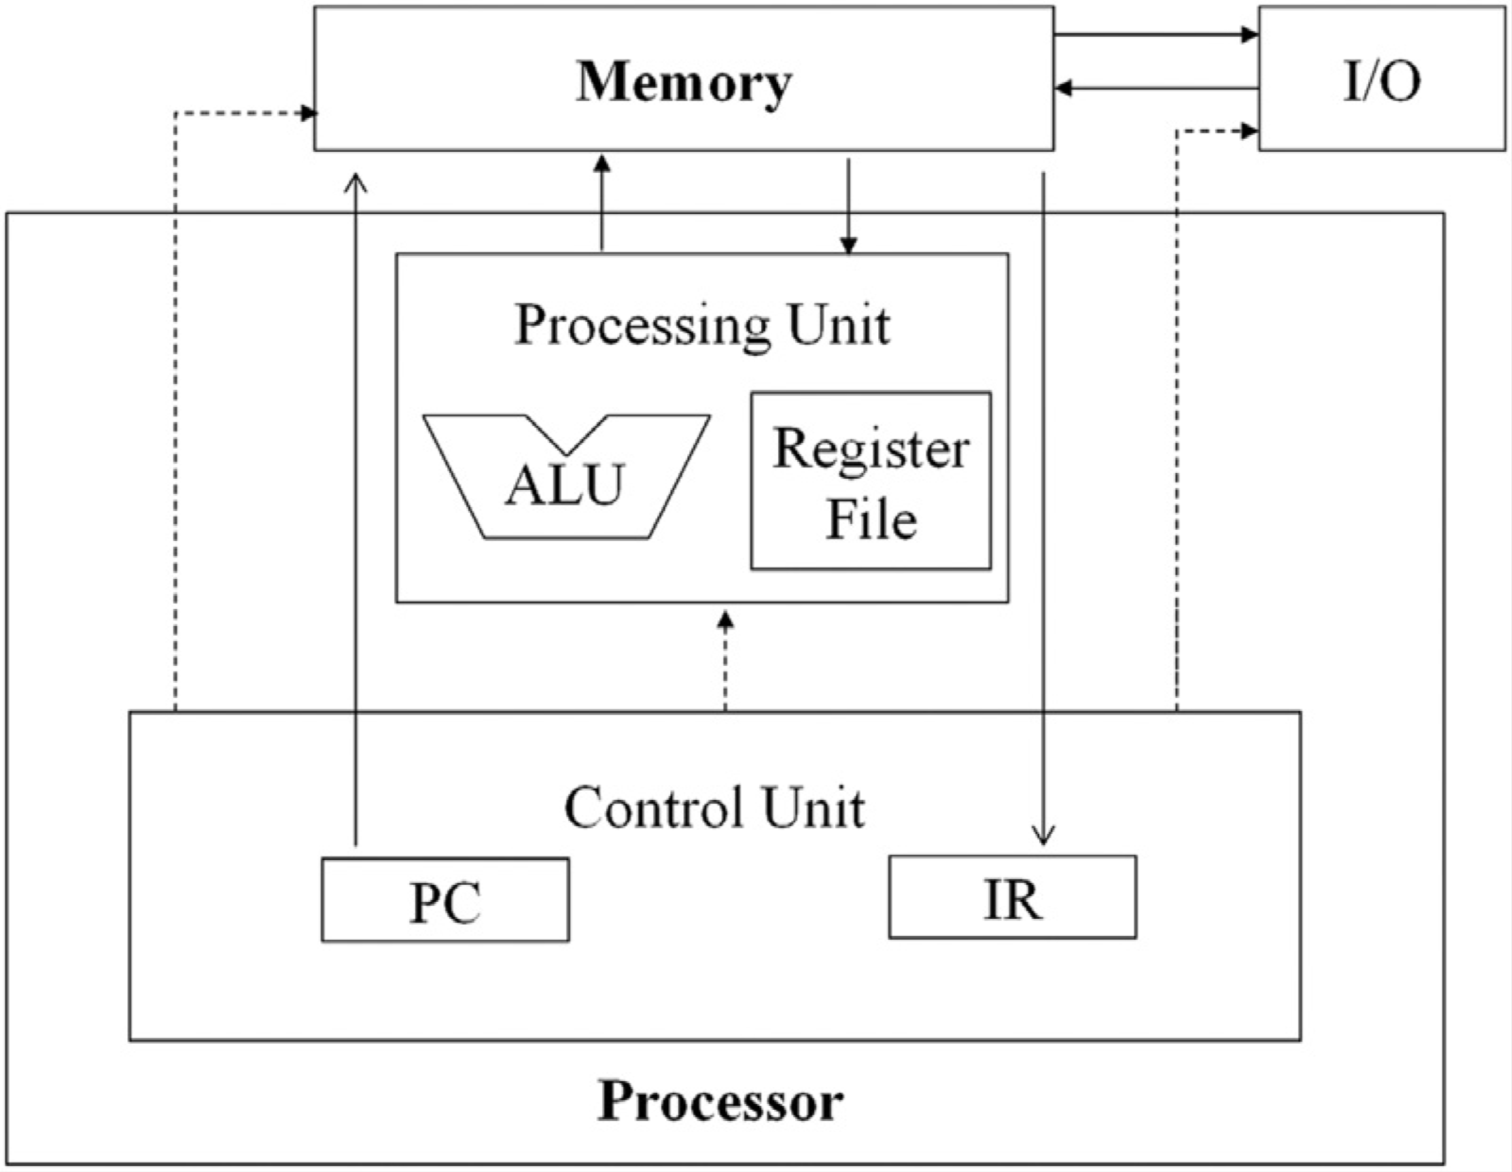
\includegraphics[width=0.9\textwidth]{figs/F4-a.1.png}
\end{figure}

该程序由指令集合组成。 控制单元维护一个程序计数器(PC),其中包含下一条要执行的指令的存储器地址。 
在每个“指令周期”中,控制单元使用 PC 将指令提取到指令寄存器 (IR) 中。 然后检查指令位以确定计算机所有组件要采取的操作。 
这就是该模型也被称为“存储程序”模型的原因,这意味着用户可以通过将不同的程序存储到计算机的内存中来改变计算机的行为。

下面修改后的冯诺依曼模型说明了将线程作为warp执行的动机,该模型经过修改以反映 GPU 设计。 
处理器对应于图 4.8 中的处理块,只有一个用于获取和分派指令的控制单元。 
相同的控制信号(图 4.8 中从控制单元到处理单元的箭头)发送到多个处理单元,
每个处理单元对应 SM 中的一个核心,每个处理单元执行 warp 中的一个线程。

\begin{figure}[H]
	\centering
	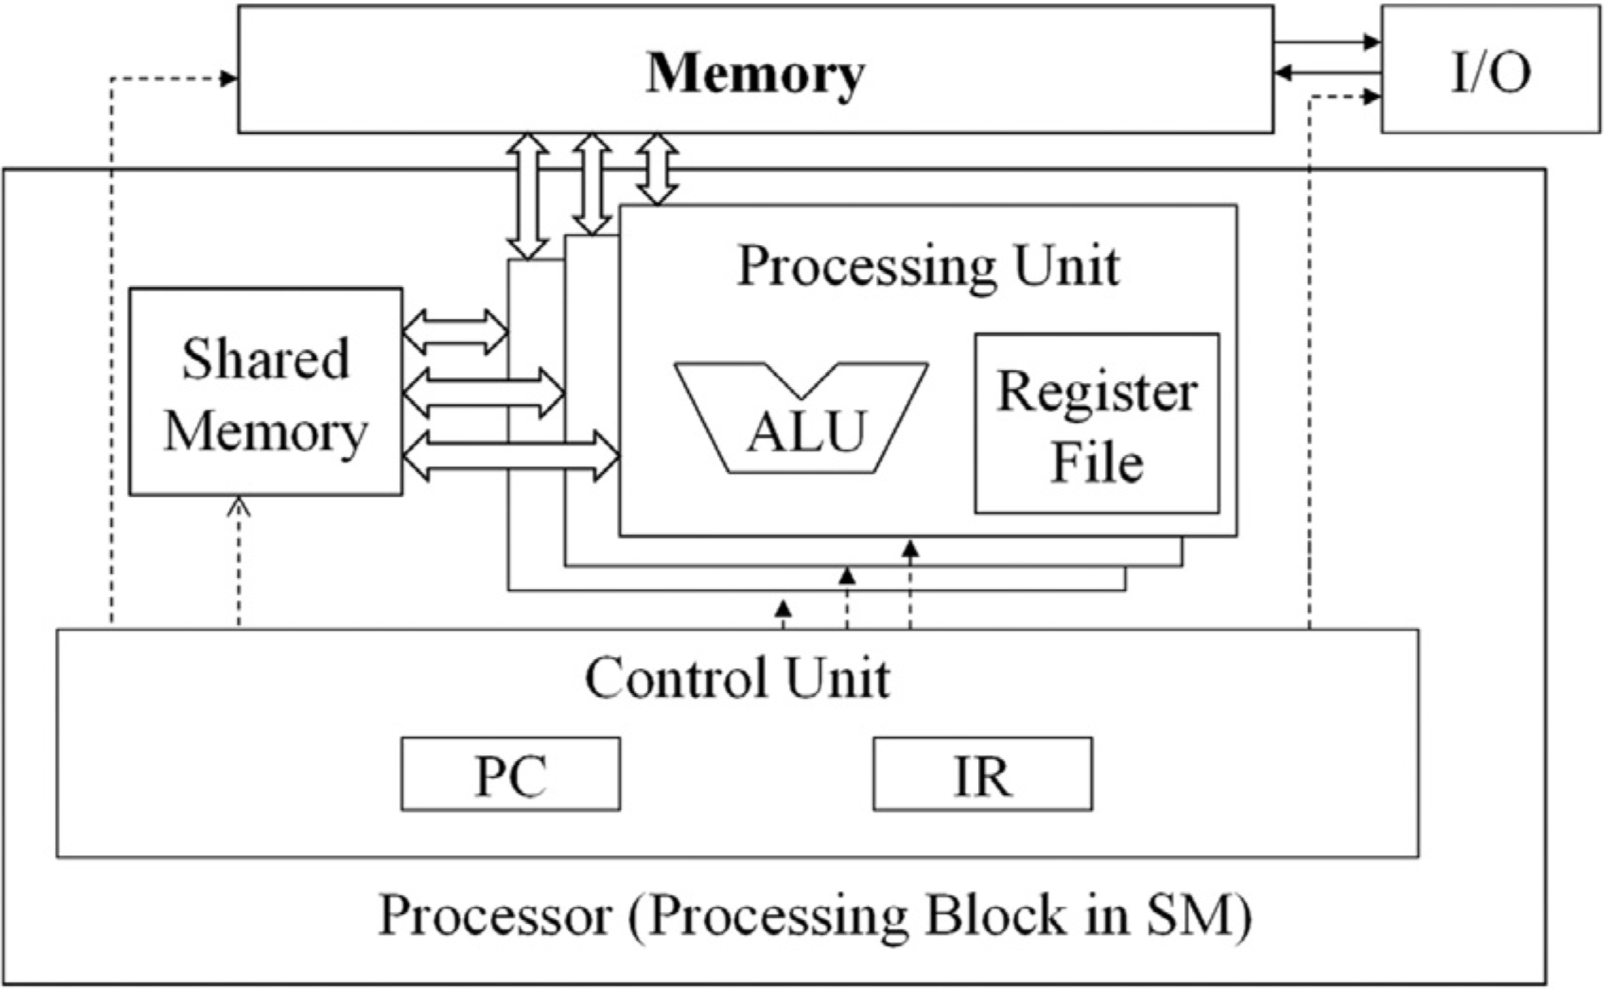
\includegraphics[width=0.9\textwidth]{figs/F4-a.2.png}
\end{figure}

由于所有处理单元均由控制单元的指令寄存器(IR)中的相同指令控制,
因此它们的执行差异是由于寄存器文件中的数据操作数值不同而造成的。 这在处理器设计中称为单指令多数据(SIMD)。 
例如,虽然所有的处理单元(核)都是由一条指令来控制的,如add r1、r2、r3,但是在不同的处理单元中,r2和r3的内容是不同的。

现代处理器中的控制单元非常复杂,包括用于获取指令的复杂逻辑和指令缓存的访问端口。 
多个处理单元共享一个控制单元可以显着降低硬件制造成本和功耗。
\end{remark}

\subsection{控制分支发散}
当 warp 内的所有线程在处理数据时遵循相同的执行路径(更正式地称为控制流)时,SIMD 执行效果良好。 
例如,对于 if-else 构造,当 warp 中的所有线程都执行 if-path 或全部执行 else-path 时,执行效果良好。 
然而,当 warp 内的线程采用不同的控制流路径时,SIMD 硬件将多次通过这些路径,每条路径一次。 
例如,对于 if-else 构造,如果 warp 中的某些线程遵循 if-path,而其他线程遵循 else 路径,则硬件将进行两次传递。 
一轮执行 if 路径后面的线程,另一遍执行 else 路径后面的线程。 在每次传递期间,不允许遵循其他路径的线程生效。

当同一 warp 中的线程遵循不同的执行路径时,我们说这些线程表现出控制发散,即它们在执行中出现发散。 
发散warp执行的多通道方法扩展了 SIMD 硬件实现 CUDA 线程完整语义的能力。 虽然硬件对 warp 中的所有线程执行相同的指令,
但它有选择地让这些线程仅在与它们所采用的路径相对应的通道中生效,从而允许每个线程看起来都采用自己的控制流路径。 
这保留了线程的独立性,同时利用了 SIMD 硬件成本降低的优势。 
然而,发散的代价是硬件需要采取额外的传递来允许warp中的不同线程做出自己的决定,以及每个传递中不活动线程消耗的执行资源。

\begin{figure}[H]
	\centering
	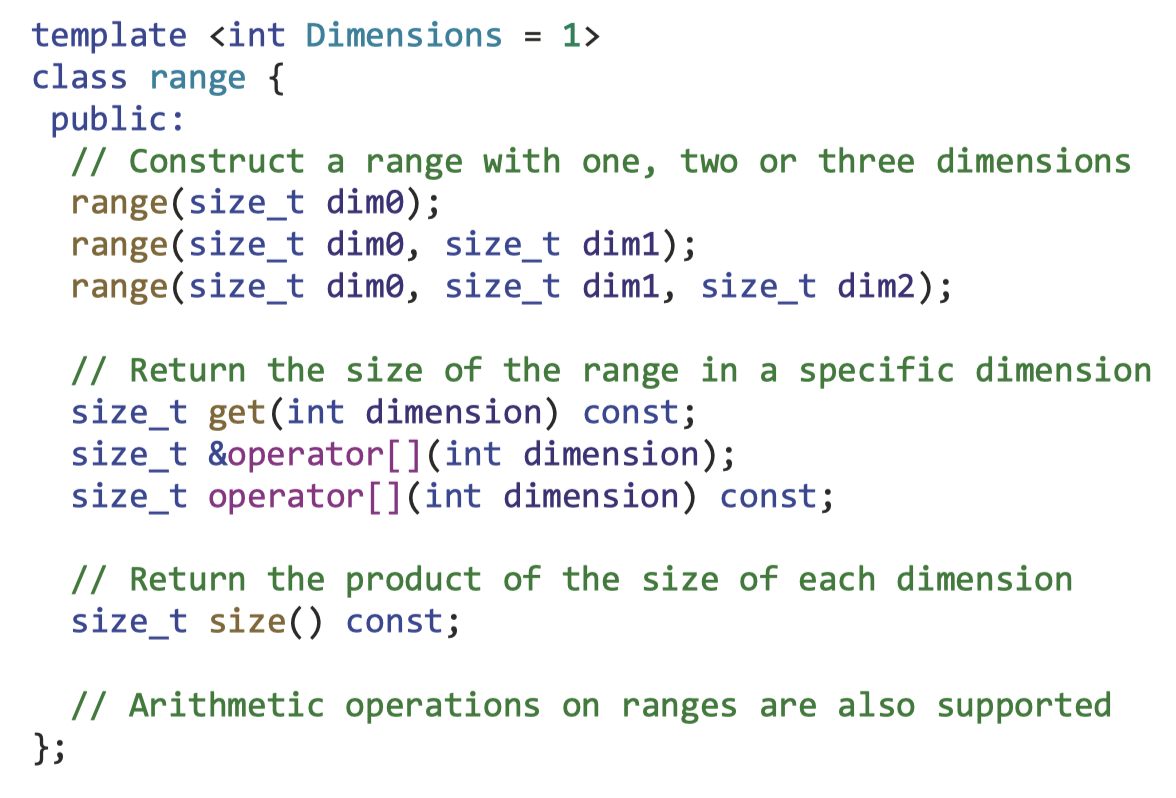
\includegraphics[width=0.9\textwidth]{figs/F4.9.png}
	\caption{\textit{在 if-else 语句处 warp 发散的示例。}}
\end{figure}

图 4.9 显示了 warp 如何执行发散的 if-else 语句的示例。 
在此示例中,当由线程 0-31 组成的 warp 到达 if-else 语句时,线程 0-23 采用 then-path,
而线程 24-31 采用 else-path。 在这种情况下,warp 将遍历代码,其中线程 0-23 执行 A,
而线程 24-31 处于非活动状态。 warp 还将再次执行代码,其中线程 24-31 执行 B,而线程 0-23 不活动。 
然后,warp 中的线程重新聚合并执行 C。在 Pascal 体系结构和先前的体系结构中,这些通道按顺序执行,
这意味着一个通道执行完成后,然后执行另一通道。 从 Volta 架构开始,各遍可以同时执行,
这意味着一个遍的执行可以与另一遍的执行交错。 此功能称为独立线程调度。 
有兴趣的读者可参阅 Volta V100 架构白皮书(NVIDIA,2017)了解详细信息。

\begin{figure}[H]
	\centering
	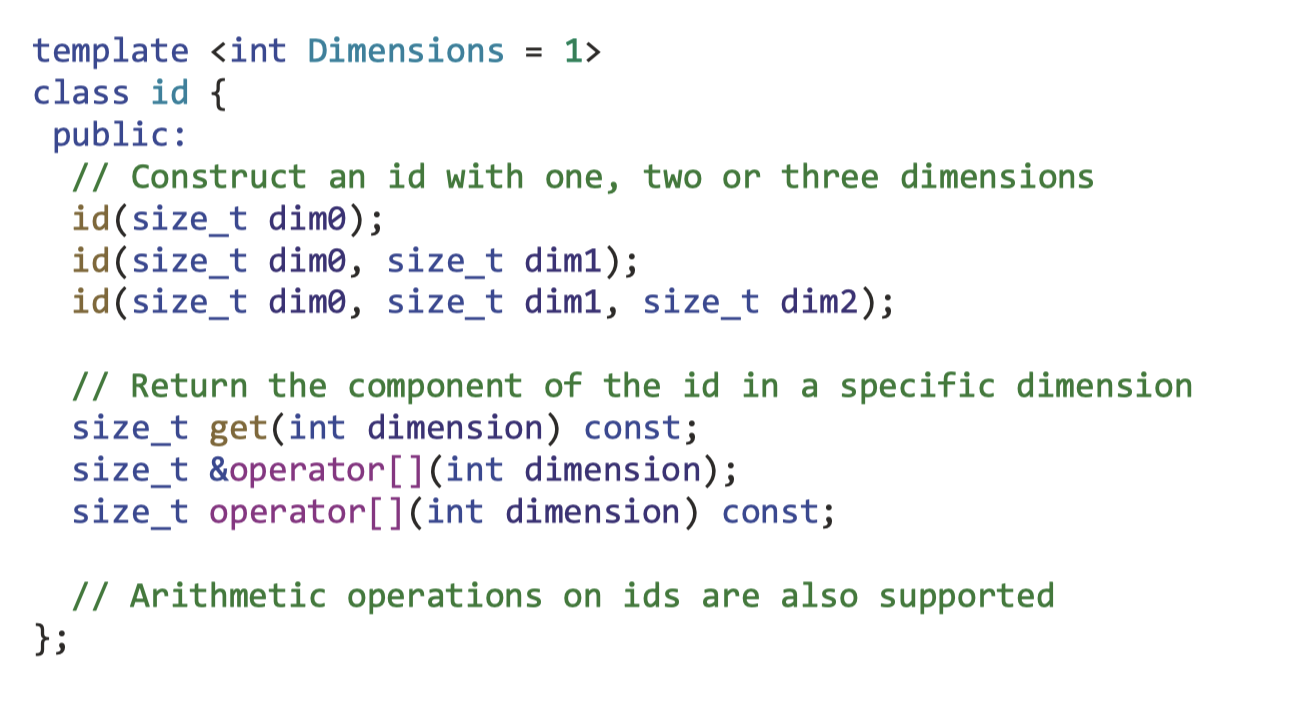
\includegraphics[width=0.9\textwidth]{figs/F4.10.png}
	\caption{\textit{for 循环中 warp 发散的示例。}}
\end{figure}

其他控制流结构中也可能出现分支。 图 4.10 显示了 warp 如何执行发散 for 循环的示例。 
在此示例中,每个线程执行不同数量的循环迭代,其范围在四到八之间。 对于前四次迭代,所有线程都处于活动状态并执行 A。
对于剩余的迭代,一些线程执行 A,而其他线程则处于非活动状态,因为它们已完成迭代。

通过检查其决策条件,可以确定控制结构是否会导致线程发散。 如果决策条件基于 threadIdx 值,则控制语句可能会导致线程发散。 
例如,语句 if(threadIdx.x > 2){...} 导致块的第一个warp中的线程遵循两个不同的控制流路径。 
线程 0、1 和 2 遵循与线程 3、4、5 等不同的路径。 同样,如果循环条件基于线程索引值,则循环可能会导致线程发散。

使用具有线程控制分支的控制构造的一个普遍原因是将线程映射到数据时处理边界条件。 
这通常是因为线程总数需要是线程块大小的倍数,而数据的大小可以是任意数字。 
从第 2 章“异构数据并行计算”中的向量加法内核开始,我们在 addVecKernel 中有一个 if(i, n) 语句。 
这是因为并非所有向量长度都可以表示为块大小的倍数。 例如,假设向量长度为 1003,我们选择 64 作为块大小。 
需要启动 16 个线程块来处理所有 1003 个向量元素。 然而,16 个线程块将有 1024 个线程。 
我们需要禁止线程块 15 中的最后 21 个线程执行原始程序不期望或不允许的工作。 
请记住,这 16 个块被划分为 32 个warp。 只有最后一个warp(即最后一个块中的第二个warp)才会有控制发散。

请注意,控制分支对性能的影响随着正在处理的向量大小的增加而减小。 对于长度为 100 的矢量,四个warp之一将具有控制发散,
这会对性能产生重大影响。 对于大小为 1000 的矢量,32 个warp中只有一个具有控制散度。 
也就是说,控制发散只会影响大约3\%的执行时间。 即使将 warp 的执行时间加倍,对总执行时间的净影响也将约为 3\%。 
显然,如果向量长度为 10,000 或更长,则 313 个warp中只有一个具有控制发散。 控制偏差的影响将远小于1%!

对于二维数据,例如第 3 章“多维网格和数据”中的彩色到灰度转换示例,if 语句还用于处理在数据边缘操作的线程的边界条件。 
在图 3.2 中,为了处理 $62 \times 76$ 图像,我们使用了 $20 = 4 \times 5$ 个二维块,
每个块由 $16 \times 16$ 个线程组成。 
每个块将被划分为8个warp; 每一个由两行块组成。 总共涉及 160 个经线(每块 8 个经线)。 分析控制发散的影响,参见图3.5。 
区域 1 的 12 个区块中的warp都不会出现控制分支。 区域 1 有 $12 \times 8 = 96$ 个warp。
对于区域 2,所有 24 个warp都将具有控制发散。 对于区域 3,所有底部warp都映射到完全位于图像外部的数据。 
结果,它们都不会通过 if 条件。 读者应该验证如果图片在垂直维度上有奇数个像素,这些warp将具有控制发散。 
在区域 4 中,前 7 个经线将具有控制发散,但最后一个经线不会。 总而言之,160 个warp中的 31 个将出现控制分支。

同样,随着水平维度中像素数量的增加,控制发散对性能的影响也会降低。 
例如,如果我们用 $16 \times 16$ 个块处理 $200 \times 150$ 个图片,
则总共会有 $130 = 13 \times 10$ 个线程块或 1040 个warp。 
区域 1 至 4 中的warp数量将为 $864(12 \times 9 \times 8)$、$72(9 \times 8)$、
$96 (12 \times 8)$和 $8(1 \times 8)$。 
这些warp中只有 80 个具有控制发散。 因此,控制发散对性能的影响将小于 8\%。 
显然,如果我们处理水平维度超过1000像素的真实图片,控制发散对性能的影响将小于2\%。

控制发散的一个重要含义是,不能假设 warp 中的所有线程都具有相同的执行时序。 
因此,如果 warp 中的所有线程必须完成其执行的一个阶段才能继续执行,
则必须使用屏障同步机制(例如 \_\_syncwarp())来确保正确性。

\subsection{warp调度和延迟容忍}
当线程分配给 SM 时,分配给 SM 的线程数通常多于 SM 中的内核数。 也就是说,
每个 SM 仅具有足够的执行单元来执行在任何时间点分配给它的所有线程的子集。 
在早期的 GPU 设计中,每个 SM 在任何给定时刻只能针对单个warp执行一条指令。 
在最近的设计中,每个 SM 都可以在任何给定时间点执行少量warp的指令。 
在任一情况下,硬件只能执行 SM 中所有warp的子集的指令。 一个合理的问题是,如果 SM 在任何时刻只能执行其中的一个子集,
为什么我们需要将如此多的 warp 分配给 SM? 答案是,这就是 GPU 容忍全局内存访问等长延迟操作的方式。

当warp要执行的指令需要等待先前启动的长延迟操作的结果时,不会选择warp来执行。 
相反,将选择另一个不再等待先前指令结果的常驻warp来执行。 如果多个 warp 准备好执行,则使用优先级机制来选择一个来执行。 
这种用其他线程的工作来填充某些线程的操作延迟时间的机制通常称为“延迟容忍”或“延迟隐藏”(请参阅“延迟容忍”边栏)。

\begin{remark}[延迟容忍]
在许多日常情况下都需要延迟容忍。 例如,在邮局,每个试图运送包裹的人最好在前往服务柜台之前填写所有表格和标签。 
然而,正如我们大家都经历过的那样,有些人等待服务台服务员告诉他们要填写哪张表格以及如何填写表格。

当服务台前排起长队时,最大限度地提高服务人员的工作效率非常重要。 让一个人在店员面前填写表格,而每个人都在等待,
这不是一个好方法。 当该人填写表格时,店员应该帮助下一个排队等候的顾客。 
这些其他客户已“准备好出发”,不应被需要更多时间填写表格的客户阻止。

这就是为什么一个好的店员会礼貌地要求第一位顾客退到一边填写表格,而店员则为其他顾客提供服务。 
在大多数情况下,第一个顾客填写完表格后,店员就会为当前顾客提供服务,而不是走到队伍的末尾。

我们可以将这些邮局客户视为warp,将职员视为硬件执行单元。 
需要填写表格的客户对应于一个warp,其持续执行依赖于长延迟操作。
\end{remark}

请注意,warp 调度还用于容忍其他类型的操作延迟,例如流水线浮点算术和分支指令。 
有了足够的warp,硬件可能会在任何时间点找到一个warp来执行,从而充分利用执行硬件,
同时某些warp的指令等待这些长延迟操作的结果。 选择准备执行的 warp 不会在执行时间线中引入任何空闲或浪费的时间,
这称为零开销线程调度(请参阅“线程、上下文切换和零开销调度”边栏) 。 
通过 warp 调度,warp 指令的漫长等待时间通过执行其他 warp 的指令来“隐藏”。 
这种容忍长操作延迟的能力是 GPU 不像 CPU 那样将尽可能多的芯片区域用于缓存和分支预测机制的主要原因。 
因此,GPU 可以将更多芯片区域用于浮点执行和内存访问通道资源。

\begin{remark}[线程、上下文切换和零开销调度]
基于冯·诺依曼模型,我们准备更深入地了解线程是如何实现的。 
现代计算机中的线程是一个程序以及在冯·诺依曼处理器上执行该程序的状态。 
回想一下,线程由程序代码、正在执行的代码中的指令以及其变量和数据结构的值组成。

在基于冯·诺依曼模型的计算机中,程序的代码存储在内存中。 PC 跟踪正在执行的程序的指令地址。 
IR 保存正在执行的指令。 寄存器和存储器保存变量和数据结构的值。

现代处理器的设计允许上下文切换,其中多个线程可以通过轮流取得进展来分时共享处理器。 
通过仔细保存和恢复PC值以及寄存器和内存的内容,我们可以暂停线程的执行并在稍后正确地恢复线程的执行。 
然而,在这些处理器中的上下文切换期间保存和恢复寄存器内容可能会在增加执行时间方面产生显着的开销。

零开销调度是指 GPU 能够将需要等待长延迟指令结果的 warp 置于休眠状态,并激活准备就绪的 warp,
而不会在处理单元中引入任何额外的空闲周期。 传统CPU会产生这样的空闲周期,
因为将执行从一个线程切换到另一线程需要将执行状态(例如传出线程的寄存器内容)保存到内存并从内存加载传入线程的执行状态。 
GPU SM 通过在硬件寄存器中保存分配的warp的所有执行状态来实现零开销调度,因此从一个warp切换到另一warp时无需保存和恢复状态。
\end{remark}

为了使延迟容忍有效,需要为 SM 分配比其执行资源可同时支持的线程多得多的线程,
以最大程度地找到在任何时间点准备好执行的 warp 的机会。 例如,在 Ampere A100 GPU 中,SM 有 64 个核心,
但最多可以同时分配 2048 个线程。 因此,SM 分配的线程数最多可比其内核在任何给定时钟周期支持的线程数多 32 倍。 
这种对 SM 的线程超额订阅对于延迟容忍至关重要。 当当前执行的warp遇到长延迟操作时,它增加了找到另一个warp执行的机会。

\subsection{资源划分和占用}
我们已经看到,为了容忍长延迟操作,最好将许多warp分配给 SM。 然而,可能并不总是可以向 SM 分配 SM 支持的最大warp数。 
分配给 SM 的warp数量与其支持的最大数量的比率称为占用率。 
要了解什么可能会阻止 SM 达到最大占用率,首先了解 SM 资源的划分方式非常重要。

SM 中的执行资源包括寄存器、共享内存(在第 5 章内存架构和数据局部性中讨论)、线程块槽和线程槽。 
这些资源在线程之间动态分区以支持它们的执行。 
例如,Ampere A100 GPU 最多可支持每个 SM 32 个块、每个 SM 64 个warp(2048 个线程)以及每个块 1024 个线程。 
如果启动的网格的块大小为 1024 个线程(允许的最大值),则每个 SM 中的 2048 个线程槽将被划分并分配给 2 个块。 
在这种情况下,每个SM最多可以容纳2个块。 类似地,如果以 512、256、128 或 64 个线程的块大小启动网格,
则 2048 个线程槽将被分区并分别分配给 4、8、16 或 32 个块。

这种在块之间动态划分线程槽的能力使得 SM 具有多种用途。 它们可以执行多个块,每个块具有几个线程,也可以执行几个块,
每个块具有多个线程。 这种动态分区可以与固定分区方法形成对比,在固定分区方法中,无论其实际需求如何,
每个块都将接收固定数量的资源。 当块需要的线程少于固定分区支持的线程并且无法支持需要比该数量更多的线程槽的块时,固定分区会导致线程槽的浪费。

资源的动态分区可能会导致资源限制之间微妙的相互作用,从而导致资源利用不足。 这种交互可以发生在块槽和线程槽之间。 
在 Ampere A100 的示例中,我们看到块大小可以在 1024 到 64 之间变化,从而导致每个 SM 分别有 2±32 个块。 
在所有这些情况下,分配给 SM 的线程总数为 2048,这使得占用率最大化。 但是,请考虑每个块有 32 个线程的情况。 
在这种情况下,2048 个线程槽需要分区并分配给 64 个块。 然而,Volta SM 一次只能支持 32 个块插槽。 
这意味着仅使用 1024 个线程槽,即 32 个块,每个块有 32 个线程。 
本例中的占用率为(1024 个分配的线程)/(2048 个最大线程)= 50\%。 
因此,要充分利用线程槽并达到最大占用率,每个块中至少需要64个线程。

当每个块的最大线程数不能被块大小整除时,就会出现另一种可能对占用率产生负面影响的情况。 
在 Ampere A100 的示例中,我们看到每个 SM 最多可支持 2048 个线程。 
但是,如果选择块大小为 768,则 SM 将只能容纳 2 个线程块(1536 个线程),从而留下 512 个线程槽位未利用。 
在这种情况下,每个 SM 的最大线程数和每个 SM 的最大块数都未达到。 
本例中的占用率为(1536 个分配的线程)/(2,048 个最大线程)= 75\%。

前面的讨论没有考虑其他资源约束的影响,例如寄存器和共享内存。 我们将在第 5 章“内存架构和数据局部性”中看到,
在 CUDA 内核中声明的自动变量被放入寄存器中。 一些内核可能使用许多自动变量,而其他内核可能只使用其中的很少一些。 
因此,我们应该预料到,有些内核每个线程需要很多寄存器,有些则需要很少。 
通过跨线程动态划分 SM 中的寄存器,如果每个线程需要很少的寄存器,则 SM 可以容纳许多块;
如果每个线程需要更多的寄存器,则可以容纳更少的块。

然而,人们确实需要意识到寄存器资源限制对占用的潜在影响。 例如,Ampere A100 GPU 允许每个 SM 最多有 65,536 个寄存器。 
为了完全占用运行,每个 SM 需要足够的寄存器来容纳 2048 个线程,
这意味着每个线程不应使用超过 (65,536 个寄存器)/(2048 个线程) = 每个线程 32 个寄存器。 
例如,如果内核每个线程使用 64 个寄存器,则 65,536 个寄存器可支持的最大线程数为 1024 个线程。 
在这种情况下,无论块大小设置为多少,内核都无法满载运行。 相反,入住率最多为50\%。 
在某些情况下,编译器可能会执行寄存器溢出以减少每个线程的寄存器需求,从而提高占用率。 
然而,这通常以增加线程从存储器访问溢出寄存器值的执行时间为代价,并且可能导致网格的总执行时间增加。 
第 5 章“内存架构和数据局部性”中对共享内存资源进行了类似的分析。

假设程序员实现的内核每个线程使用 31 个寄存器,并将其配置为每个块 512 个线程。 
在这种情况下,SM 将有 (2048 个线程)/(512 个线程/块) = 4 个块同时运行。 
这些线程总共将使用 (2048 个线程) 3 (31 个寄存器/线程) = 63,488 个寄存器,这小于 65,536 个寄存器的限制。 
现在假设程序员在内核中声明另外两个自动变量,将每个线程使用的寄存器数量增加到 33 个。
2048 个线程所需的寄存器数量现在为 67,584 个寄存器,这超出了寄存器限制。
 CUDA运行时系统可以通过仅向每个SM分配3个块而不是4个块来处理这种情况,从而将所需的寄存器数量减少到50,688个寄存器。 
 但是,这会将 SM 上运行的线程数从 2048 个减少到 1536 个; 也就是说,通过使用两个额外的自动变量,
 该程序将占用率从 100\% 减少到 75\%。 这有时被称为“性能悬崖”,
 其中资源使用量的轻微增加可能会导致并行性和所实现的性能显着下降(Ryoo 等人,2008)。

读者应该清楚,所有动态分区资源的约束以复杂的方式相互作用。 准确确定每个 SM 中运行的线程数量可能很困难。 
读者可以参考 CUDA 占用计算器(CUDA 占用计算器,Web),它是一个可下载的电子表格,
在给定内核资源使用情况的情况下,计算特定设备实现的每个 SM 上运行的实际线程数。

\subsection{查询设备属性}
我们对 SM 资源划分的讨论提出了一个重要问题:我们如何找出特定设备可用的资源量? 当CUDA应用程序在系统上执行时,
它如何找出设备中SM的数量以及可以分配给每个SM的块和线程的数量? 同样的问题也适用于其他类型的资源,
其中一些我们迄今为止尚未讨论。 一般来说,许多现代应用程序被设计为在各种硬件系统上执行。 
应用程序通常需要查询底层硬件的可用资源和功能,以便利用功能较强的系统,
同时补偿功能较弱的系统(请参阅“资源和功能查询”边栏)。

\begin{remark}[资源和能力查询]
在日常生活中,我们经常查询环境中的资源和能力。 例如,当我们预订酒店时,我们可以查看酒店房间附带的设施。 
如果房间有吹风机,我们就不用带了。 大多数美国酒店客房都配有吹风机,而其他地区的许多酒店则没有。

一些亚洲和欧洲酒店提供牙膏甚至牙刷,而大多数美国酒店则不提供。 
美国很多酒店同时提供洗发水和护发素,而其他大洲的酒店往往只提供洗发水。

如果房间里有微波炉和冰箱,我们就可以把晚餐剩下的东西拿走,第二天再吃。 
如果酒店有游泳池,我们可以带泳衣,商务会议结束后去畅游。 如果酒店没有游泳池但有健身房,我们可以带跑鞋和运动服。 
一些亚洲高端酒店甚至提供运动服!

这些酒店设施是酒店财产、资源和能力的一部分。 经验丰富的旅客会在酒店网站上查看酒店情况,
选择最符合自己需求的酒店,并更高效、更有效地打包行李。
\end{remark}

每个 CUDA 设备 SM 中的资源量被指定为设备计算能力的一部分。 一般来说,计算能力级别越高,每个SM中可用的资源就越多。 
GPU 的计算能力往往会一代又一代地增强。 Ampere A100 GPU 的计算能力为 8.0。

在 CUDA C 中,主机代码有一个内置机制来查询系统中可用设备的属性。 
CUDA运行时系统(设备驱动程序)有一个API函数cudaGetDeviceCount,它返回系统中可用的CUDA设备的数量。 
主机代码可以使用以下语句找出可用的 CUDA 设备的数量:

int devCount;

cudaGetDeviceCount(\&devCount);

虽然这可能并不明显,但现代 PC 系统通常有两个或更多 CUDA 设备。 这是因为许多 PC 系统都配备了一个或多个“集成”GPU。 
这些 GPU 是默认图形单元,提供基本功能和硬件资源,以便为现代基于窗口的用户界面执行最少的图形功能。 
大多数 CUDA 应用程序在这些集成设备上的性能都不会很好。 
这将是主机代码迭代所有可用设备、查询其资源和功能并选择具有足够资源来执行性能令人满意的应用程序的原因。

CUDA 运行时对系统中所有可用设备进行编号,从 0 到 devCount-1。 
它提供了一个 API 函数 cudaGetDeviceProperties,该函数返回其编号作为参数给出的设备的属性。 
例如,我们可以在主机代码中使用以下语句来迭代可用设备并查询其属性:

\begin{figure}[H]
	\centering
	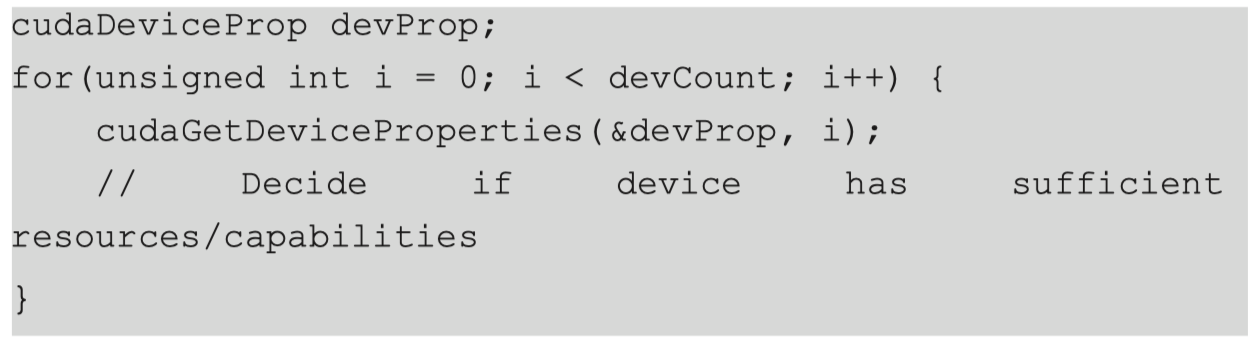
\includegraphics[width=0.9\textwidth]{figs/F4-a.3.png}
\end{figure}

内置类型 cudaDeviceProp 是一个 C 结构类型,其字段表示 CUDA 设备的属性。 
读者可参考《CUDA C 编程指南》了解该类型的所有字段。 我们将讨论其中一些与向线程分配执行资源特别相关的字段。 
我们假设属性在 devProp 变量中返回,其字段由 cudaGetDeviceProperties 函数设置。 
如果读者选择以不同的方式命名变量,那么在下面的讨论中显然需要替换适当的变量名称。

顾名思义,字段 devProp.maxThreadsPerBlock 给出了查询设备中的块中允许的最大线程数。 
某些设备允许每个块中最多有 1024 个线程,而其他设备可能允许更少。 未来的设备甚至可能允许每个块超过 1024 个线程。 
因此,就应用程序而言,最好查询可用设备并确定哪些设备将在每个块中允许足够数量的线程。

设备中 SM 的数量在 devProp.multiProcessorCount 中给出。 
如果应用程序需要许多 SM 才能达到令人满意的性能,则一定要检查预期设备的此属性。 
此外,设备的时钟频率位于 devProp.clockRate 中。 时钟速率和 SM 数量的组合可以很好地指示设备的最大硬件执行吞吐量。

主机代码可以在字段 devProp.maxThreadsDim[0](对于 x 维度)、
devProp.maxThreadsDim[1](对于 y 维度)
和 devProp.maxThreadsDim[2](对于 z 维度)中找到沿着块的每个维度允许的最大线程数。 
使用此信息的一个示例是自动调整系统在评估底层硬件的最佳性能块尺寸时设置块尺寸的范围。 
类似地,它可以在 devProp 中找到网格每个维度上允许的最大块数。 
maxGridSize[0](对于 x 维度)、devProp.maxGridSize[1](对于 y 维度)和 devProp.maxGridSize[2](对于 z 维度)。 
此信息的典型用途是确定网格是否可以有足够的线程来处理整个数据集,或者是否需要某种迭代方法。

字段 devProp.regsPerBlock 给出了每个 SM 中可用的寄存器数量。 
该字段可用于确定内核是否可以在特定设备上实现最大占用率,或者是否会受到其寄存器使用的限制。 
请注意,该字段的名称有点误导。 对于大多数计算能力级别,块可以使用的最大寄存器数量实际上与 SM 中可用的寄存器总数相同。 
然而,对于某些计算能力级别,块可以使用的最大寄存器数量小于 SM 上可用的寄存器总数。

我们还讨论了warp的大小取决于硬件。 warp的大小可以从 devProp.warpSize 字段获得。

cudaDeviceProp 类型中还有更多字段。 我们将在整本书中讨论它们,同时介绍它们旨在反映的概念和功能。

\subsection{总结}
GPU 被组织成 SM,它由共享控制逻辑和内存资源的多个核心处理块组成。 
当网格启动时,其块会以任意顺序分配给 SM,从而实现 CUDA 应用程序的透明可扩展性。 
透明的可扩展性有一个限制:不同块中的线程无法相互同步。

线程被分配给 SM 来逐块执行。 一旦一个块被分配给 SM,它就会被进一步划分为 warp。 
warp 中的线程按照 SIMD 模型执行。 如果同一 warp 中的线程因采用不同的执行路径而发散,则处理块会分步执行这些路径,
其中每个线程仅在与其所采用的路径相对应的遍中处于活动状态。

SM 分配给它的线程可能比它可以同时执行的线程多得多。 在任何时候,SM 都只执行其常驻warp的一小部分指令。 
这允许其他线程等待长延迟操作,而不会减慢大量处理单元的整体执行吞吐量。 
分配给SM的线程数与它可以支持的最大线程数的比率称为占用率。 SM的占用率越高,越能隐藏长延迟操作。

每个 CUDA 设备对每个 SM 中的可用资源量施加潜在不同的限制。 
例如,每个 CUDA 设备对其每个 SM 可容纳的块数、线程数、寄存器数以及其他资源量都有限制。 
对于每个内核来说,这些资源限制中的一个或多个都可能成为占用的限制因素。 
CUDA C 为程序员提供了在运行时查询 GPU 中可用资源的能力。

\newpage
\section{错误处理}
错误处理是 C++ 的一项关键功能。 本章讨论将工作卸载到设备(加速器)时遇到的独特错误处理挑战,
以及 SYCL 如何使我们完全可以应对这些挑战。

检测和处理意外情况和错误在应用程序开发过程中很有帮助(想想:从事该项目的其他程序员确实会犯错误),
但更重要的是在稳定和安全的生产应用程序和库中发挥关键作用。 
本章致力于描述 C++ 中可用的 SYCL 错误处理机制,以便我们能够了解我们的选项是什么,
以及如果我们关心检测和管理错误,如何构建应用程序。

本章概述了 SYCL 中的同步和异步错误,描述了如果我们在代码中不执行任何操作来处理错误,
应用程序的行为,并深入探讨允许我们处理异步错误的 SYCL 特定机制。


\subsection{安全第一}
C++ 错误处理的一个核心方面是,如果我们不采取任何措施来处理已检测到(引发)的错误,那么应用程序将终止并指示出现问题。 
这种行为使我们能够在编写应用程序时无需关注错误管理,并且仍然确信错误会以某种方式向开发人员或用户发出信号。 
当然,我们并不是建议我们应该忽略错误处理! 生产应用程序的编写应将错误管理作为架构的核心部分,
但应用程序在开始开发时通常没有这样的关注点。 
C++ 的目标是使不处理错误的代码仍然能够观察到许多错误,即使它们没有被显式处理。

由于 SYCL 是数据并行 C++,因此同样的理念成立:如果我们在代码中不采取任何措施来管理错误,并且检测到错误,
则程序将发生异常终止,让我们知道发生了错误。 生产应用程序当然应该将错误管理视为软件架构的核心部分,不仅要报告,
而且通常还要从错误情况中恢复。

\begin{remark}
	如果我们不添加任何错误管理代码并且发生错误,我们仍然会看到程序异常终止,这表明需要进行更深入的研究。
\end{remark}

\subsection{错误类型}
C++ 通过其异常机制提供了一个用于通知和处理错误的框架。 
除此之外,异构编程还需要额外级别的错误管理,因为设备上或尝试在设备上启动工作时会发生一些错误。 
这些错误通常与主机程序的执行及时分离,因此它们不能与常规 C++ 异常处理机制干净地集成。 
为了解决这个问题,有额外的机制可以使异步错误像典型的 C++ 异常一样易于管理和控制。

图 5-1 显示了典型应用程序的两个组件:(1) 主机代码按顺序运行并将工作提交到任务图以供将来执行;
(2) 任务图与主机程序异步运行并执行内核或其他程序 当满足必要的依赖性时对设备执行的操作。 
该示例显示了parallel\_for作为任务图的一部分异步执行的操作,但其他操作也是可能的,并在第3、4和8章中讨论。

图 5-1 左右(主机和任务图)之间的区别是理解同步错误和异步错误之间差异的关键。

当主机程序执行操作(例如 API 调用或对象构造)时检测到错误条件时,就会发生同步错误。 
它们可以在图左侧的指令完成之前被检测到,并且导致错误的操作可以立即抛出错误。 
我们可以使用 try-catch 构造将特定指令包装在图的左侧,
期望在 try 块结束之前检测到由于 try 内的操作而发生的错误(并因此捕获)。 
C++ 异常机制旨在准确处理这些类型的错误。

异步错误发生在图 5-1 右侧的部分,只有在执行任务图中的操作时才会检测到错误。 
当异步错误作为任务图执行的一部分被检测到时,主机程序通常已经继续执行,
因此没有代码可以用 try-catch 结构包装来捕获这些错误。 
相反,SYCL 中有一个异步异常处理框架来处理这些相对于主机程序执行看似随机且不受控制的时间发生的错误。

\subsection{让我们创建一些错误!}
作为本章剩余部分的示例并允许我们进行实验,我们将在以下示例中创建同步和异步错误。

\subsubsection{同步错误}
在图 5-2 中,从缓冲区创建了一个子缓冲区,但其大小非法(大于原始缓冲区)。 
子缓冲区的构造函数检测到此错误并在构造函数执行完成之前抛出异常。 
这是一个同步错误,因为它是作为主机程序执行的一部分(同步)发生的。 
在构造函数返回之前可以检测到错误,因此可以在错误的起源点或在主机程序中检测到错误时立即对其进行处理。

我们的代码示例没有执行任何操作来捕获和处理 C++ 异常,
因此默认的 C++ 未捕获异常处理程序为我们调用 std::terminate,表示出现了问题。

\subsubsection{异步错误}
生成异步错误有点棘手,因为实现会尽可能努力同步检测和报告错误。 
同步错误更容易调试,因为它们发生在主机程序中的特定起始点,因此只要有可能,它们都是实现的首选。 
出于演示目的,生成异步错误的一种方法是在主机任务内引发异常,该任务作为任务图的一部分异步执行。 
图 5-3 演示了此类异常。 异步错误在许多情况下都可能发生并报告,因此请注意,
图 5-3 中所示的主机任务示例只是一种可能性,而不是异步错误的要求。

\subsection{应用程序错误处理策略}
C++ 异常功能旨在将程序中检测到错误的点与可能处理错误的点清楚地分开,并且此概念非常适合 SYCL 中的同步错误和异步错误。 
通过抛出和捕获机制,可以定义处理程序的层次结构,这在生产应用程序中非常重要。

构建能够以一致且可靠的方式处理错误的应用程序需要预先制定策略以及为错误管理而构建的软件架构。 
C++ 提供了灵活的工具来实现许多替代策略,但这种架构超出了本章的范围。 
有许多书籍和其他参考文献专门讨论此主题,因此我们鼓励您查阅它们以全面了解 C++ 错误管理策略。

也就是说,错误检测和报告并不总是需要达到生产规模。 如果目标只是在执行期间检测错误并报告错误(但不一定要从中恢复),
则可以通过最少的代码可靠地检测和报告程序中的错误。 
以下各节首先介绍如果我们忽略错误处理并且不执行任何操作(默认行为并没有那么糟糕!)会发生什么,
然后是在基本应用程序中易于实现的推荐错误报告。

\subsubsection{忽略错误处理}
C++ 和 SYCL 旨在告诉我们,即使我们没有显式处理错误,也会出现问题。 
未处理的同步或异步错误的默认结果是程序异常终止,操作系统应该告诉我们这一点。 
以下两个示例分别模拟了如果我们不处理同步错误和异步错误时将发生的行为。

图 5-4 显示了未处理的 C++ 异常的结果,例如,该异常可能是未处理的 SYCL 同步错误。 
我们可以使用此代码来测试特定操作系统在这种情况下会报告什么。

图 5-5 显示了调用 std::terminate 的示例输出,这将是我们的应用程序中未处理的 SYCL 异步错误的结果。 
我们可以使用此代码来测试特定操作系统在这种情况下会报告什么。

尽管我们应该处理程序中的错误,但未捕获的异常最终会被捕获并终止程序,这比异常被默默地丢失要好!

\subsubsection{同步错误处理}
我们将本节保持得非常简短,因为 SYCL 同步错误只是 C++ 异常。 
SYCL 中添加的大多数附加错误机制与我们在下一节中介绍的异步错误相关,但同步错误很重要,因为实现尝试同步检测和报告尽可能多的错误,因为它们更容易推理和处理。

SYCL 定义的同步错误属于 sycl::exception 类型,它是一个从 std::exception 派生的类,
它允许我们通过 try-catch 结构专门捕获 SYCL 错误,如图 5-6 所示。

在 C++ 错误处理机制之上,SYCL 为运行时抛出的异常添加了 sycl::exception 类型。 
其他一切都是标准 C++ 异常处理,因此大多数开发人员都会熟悉。

图 5-7 中提供了一个稍微更完整的示例,其中处理了其他类别的异常。

\subsubsection{异步错误处理}
异步错误由 SYCL 运行时(或底层后端)检测,并且错误的发生独立于主机程序中命令的执行。 
错误存储在 SYCL 运行时内部的列表中,并且仅在程序员可以控制的特定点释放以进行处理。 
我们需要讨论两个主题来讨论异步错误的处理:

\begin{enumerate}
	\item 当处理未完成的异步错误时,处理程序应该做什么
	\item 当异步处理程序被调用时
\end{enumerate}

\subsubsection{异步处理程序}
异步处理程序是应用程序定义的函数,它注册到 SYCL 上下文和/或队列。 
在下一节定义的时间,如果有任何未处理的异步异常可供处理,则 SYCL 运行时将调用异步处理程序并传递这些异常的列表。

异步处理程序作为 std::function 传递到上下文或队列构造函数,
并且可以根据我们的偏好以常规函数、lambda 表达式或函数对象等方式进行定义。 
该处理程序必须接受 sycl::exception\_list 参数,如图 5-8 所示的示例处理程序所示。

在图 5-8 中,std::rethrow\_exception 后跟特定异常类型的 catch 提供了异常类型的过滤,
在本例中仅过滤 sycl::exception。 我们还可以使用 C++ 中的替代过滤方法,或者只选择处理所有异常,无论其类型如何。

处理程序在构造时与队列或上下文相关联(第 6 章中详细介绍了低级细节)。 
例如,要将图 5-8 中定义的处理程序注册到我们正在创建的队列中,我们可以编写

queue my\_queue{ gpu\_selector\_v, handle\_async\_error };

同样,要将图 5-8 中定义的处理程序注册到我们正在创建的上下文中,我们可以编写

context my\_context{handle\_async\_error };

大多数应用程序不需要显式创建或管理上下文(它们是在后台自动为我们创建的),
因此如果要使用异步处理程序,大多数开发人员应该将此类处理程序与为特定设备构建的队列相关联 (而不是明确的上下文)。

如果没有为队列或队列的父上下文定义异步处理程序,并且该队列(或上下文)发生必须处理的异步错误,则调用默认异步处理程序。 
默认处理程序的运行方式就好像它的编码如图 5-9 所示。

默认处理程序应向用户显示有关异常列表中任何错误的一些信息,
然后通过 std::terminate 结束应用程序,这应导致操作系统报告终止异常。

我们在异步处理程序中放置的内容取决于我们。 
它的范围可以从记录错误到应用程序终止,再到恢复错误条件以便应用程序可以继续正常执行。 
常见情况是通过调用 sycl::exception::what() 报告可用错误的任何详细信息,然后终止应用程序。

虽然异步处理程序在内部做什么由我们决定,但一个常见的错误是打印一条错误消息(可能会在程序中的其他消息的噪音中错过),
然后完成处理程序函数。 除非我们制定了错误管理原则,允许我们恢复已知的程序状态并确信继续执行是安全的,
否则我们应该考虑在异步处理程序函数中终止应用程序。 
这减少了检测到错误但无意中允许应用程序继续执行的程序出现错误结果的机会。 
在许多程序中,一旦我们检测到异步异常,异常终止是首选结果。

\subsubsection{处理程序的调用}
异步处理程序由运行时在特定时间调用。 
错误发生时不会立即报告,因为如果是这种情况,错误管理和安全应用程序编程(特别是多线程)
将变得更加困难和昂贵(例如,主机和设备之间的额外同步)。 相反,异步处理程序会在以下特定时间被调用:

\begin{enumerate}
	\item 当主机程序对特定队列调用queue::throw\_asynchronous()时

	\item 当主机程序对特定队列调用queue::wait\_and\_throw()时

	\item 当主机程序对特定事件调用 event::wait\_and\_throw() 时

	\item 当队列被销毁时

	\item 当上下文被破坏时
\end{enumerate}

方法 1-3 为主机程序提供了一种控制何时处理异步异常的机制,以便可以管理线程安全和特定于应用程序的其他细节。 
它们有效地提供了异步异常进入主机程序控制流的控制点,并且几乎可以像处理同步错误一样进行处理。

如果用户没有显式调用方法 1-3 之一,则在程序拆卸过程中,当队列和上下文被销毁时,通常会报告异步错误。 
这通常足以向用户发出信号,表明出现了问题并且程序结果不值得信任。

然而,依靠程序拆卸期间的错误检测并不适用于所有情况。 
例如,如果程序仅在达到某些算法收敛标准时才会终止,并且这些标准只能通过成功执行设备内核才能实现,
则异步异常可能表明该算法永远不会收敛并开始拆卸(其中错误 会被注意到)。 
在这些情况下,以及在制定了更完整的错误处理策略的生产应用程序中,
在程序中的常规和受控点调用 throw\_asynchronous() 
或 wait\_and\_throw() 是有意义的(例如,在检查算法是否收敛之前) 。

\subsection{设备上的错误}
本章讨论的错误检测和处理机制是基于主机的。 
它们是主机程序可以检测和处理主机程序中或在设备上执行内核期间可能出现问题的机制。 
我们没有讨论的是如何从我们编写的设备代码中发出信号,表明出现了问题。 这种遗漏并不是错误,而是故意的。

SYCL 明确不允许在设备代码中使用 C++ 异常处理机制(例如 throw),因为某些类型的设备会产生我们通常不想支付的性能成本。 
如果我们检测到设备代码中出现问题,我们应该使用现有的非基于异常的技术来发出错误信号。 
例如,我们可以写入一个缓冲区来记录错误或从我们定义的数值计算中返回一些无效结果,这些结果意味着发生了错误。 
在这些情况下,正确的策略是非常具体的应用程序。

\subsection{概括}
在本章中,我们介绍了同步和异步错误,介绍了如果我们不采取任何措施来管理可能发生的错误时预期的默认行为,
并介绍了用于在应用程序中的受控点处理异步错误的机制。 
错误管理策略是软件工程中的一个主要主题,并且在许多应用程序中编写的代码中占很大比例。 
SYCL 集成了我们在错误处理方面已有的 C++ 知识,并提供了灵活的机制来与我们首选的错误管理策略集成。

\end{document}


























